% Options for packages loaded elsewhere
\PassOptionsToPackage{unicode}{hyperref}
\PassOptionsToPackage{hyphens}{url}
%
\documentclass[
]{article}
\usepackage{amsmath,amssymb}
\usepackage{lmodern}
\usepackage{iftex}
\ifPDFTeX
  \usepackage[T1]{fontenc}
  \usepackage[utf8]{inputenc}
  \usepackage{textcomp} % provide euro and other symbols
\else % if luatex or xetex
  \usepackage{unicode-math}
  \defaultfontfeatures{Scale=MatchLowercase}
  \defaultfontfeatures[\rmfamily]{Ligatures=TeX,Scale=1}
\fi
% Use upquote if available, for straight quotes in verbatim environments
\IfFileExists{upquote.sty}{\usepackage{upquote}}{}
\IfFileExists{microtype.sty}{% use microtype if available
  \usepackage[]{microtype}
  \UseMicrotypeSet[protrusion]{basicmath} % disable protrusion for tt fonts
}{}
\makeatletter
\@ifundefined{KOMAClassName}{% if non-KOMA class
  \IfFileExists{parskip.sty}{%
    \usepackage{parskip}
  }{% else
    \setlength{\parindent}{0pt}
    \setlength{\parskip}{6pt plus 2pt minus 1pt}}
}{% if KOMA class
  \KOMAoptions{parskip=half}}
\makeatother
\usepackage{xcolor}
\usepackage[margin=1in]{geometry}
\usepackage{color}
\usepackage{fancyvrb}
\newcommand{\VerbBar}{|}
\newcommand{\VERB}{\Verb[commandchars=\\\{\}]}
\DefineVerbatimEnvironment{Highlighting}{Verbatim}{commandchars=\\\{\}}
% Add ',fontsize=\small' for more characters per line
\usepackage{framed}
\definecolor{shadecolor}{RGB}{248,248,248}
\newenvironment{Shaded}{\begin{snugshade}}{\end{snugshade}}
\newcommand{\AlertTok}[1]{\textcolor[rgb]{0.94,0.16,0.16}{#1}}
\newcommand{\AnnotationTok}[1]{\textcolor[rgb]{0.56,0.35,0.01}{\textbf{\textit{#1}}}}
\newcommand{\AttributeTok}[1]{\textcolor[rgb]{0.77,0.63,0.00}{#1}}
\newcommand{\BaseNTok}[1]{\textcolor[rgb]{0.00,0.00,0.81}{#1}}
\newcommand{\BuiltInTok}[1]{#1}
\newcommand{\CharTok}[1]{\textcolor[rgb]{0.31,0.60,0.02}{#1}}
\newcommand{\CommentTok}[1]{\textcolor[rgb]{0.56,0.35,0.01}{\textit{#1}}}
\newcommand{\CommentVarTok}[1]{\textcolor[rgb]{0.56,0.35,0.01}{\textbf{\textit{#1}}}}
\newcommand{\ConstantTok}[1]{\textcolor[rgb]{0.00,0.00,0.00}{#1}}
\newcommand{\ControlFlowTok}[1]{\textcolor[rgb]{0.13,0.29,0.53}{\textbf{#1}}}
\newcommand{\DataTypeTok}[1]{\textcolor[rgb]{0.13,0.29,0.53}{#1}}
\newcommand{\DecValTok}[1]{\textcolor[rgb]{0.00,0.00,0.81}{#1}}
\newcommand{\DocumentationTok}[1]{\textcolor[rgb]{0.56,0.35,0.01}{\textbf{\textit{#1}}}}
\newcommand{\ErrorTok}[1]{\textcolor[rgb]{0.64,0.00,0.00}{\textbf{#1}}}
\newcommand{\ExtensionTok}[1]{#1}
\newcommand{\FloatTok}[1]{\textcolor[rgb]{0.00,0.00,0.81}{#1}}
\newcommand{\FunctionTok}[1]{\textcolor[rgb]{0.00,0.00,0.00}{#1}}
\newcommand{\ImportTok}[1]{#1}
\newcommand{\InformationTok}[1]{\textcolor[rgb]{0.56,0.35,0.01}{\textbf{\textit{#1}}}}
\newcommand{\KeywordTok}[1]{\textcolor[rgb]{0.13,0.29,0.53}{\textbf{#1}}}
\newcommand{\NormalTok}[1]{#1}
\newcommand{\OperatorTok}[1]{\textcolor[rgb]{0.81,0.36,0.00}{\textbf{#1}}}
\newcommand{\OtherTok}[1]{\textcolor[rgb]{0.56,0.35,0.01}{#1}}
\newcommand{\PreprocessorTok}[1]{\textcolor[rgb]{0.56,0.35,0.01}{\textit{#1}}}
\newcommand{\RegionMarkerTok}[1]{#1}
\newcommand{\SpecialCharTok}[1]{\textcolor[rgb]{0.00,0.00,0.00}{#1}}
\newcommand{\SpecialStringTok}[1]{\textcolor[rgb]{0.31,0.60,0.02}{#1}}
\newcommand{\StringTok}[1]{\textcolor[rgb]{0.31,0.60,0.02}{#1}}
\newcommand{\VariableTok}[1]{\textcolor[rgb]{0.00,0.00,0.00}{#1}}
\newcommand{\VerbatimStringTok}[1]{\textcolor[rgb]{0.31,0.60,0.02}{#1}}
\newcommand{\WarningTok}[1]{\textcolor[rgb]{0.56,0.35,0.01}{\textbf{\textit{#1}}}}
\usepackage{graphicx}
\makeatletter
\def\maxwidth{\ifdim\Gin@nat@width>\linewidth\linewidth\else\Gin@nat@width\fi}
\def\maxheight{\ifdim\Gin@nat@height>\textheight\textheight\else\Gin@nat@height\fi}
\makeatother
% Scale images if necessary, so that they will not overflow the page
% margins by default, and it is still possible to overwrite the defaults
% using explicit options in \includegraphics[width, height, ...]{}
\setkeys{Gin}{width=\maxwidth,height=\maxheight,keepaspectratio}
% Set default figure placement to htbp
\makeatletter
\def\fps@figure{htbp}
\makeatother
\setlength{\emergencystretch}{3em} % prevent overfull lines
\providecommand{\tightlist}{%
  \setlength{\itemsep}{0pt}\setlength{\parskip}{0pt}}
\setcounter{secnumdepth}{-\maxdimen} % remove section numbering
\ifLuaTeX
  \usepackage{selnolig}  % disable illegal ligatures
\fi
\IfFileExists{bookmark.sty}{\usepackage{bookmark}}{\usepackage{hyperref}}
\IfFileExists{xurl.sty}{\usepackage{xurl}}{} % add URL line breaks if available
\urlstyle{same} % disable monospaced font for URLs
\hypersetup{
  pdftitle={Predator, prey and strandings: An IBM approach to modelling the `Blue Fleet'},
  pdfauthor={J.M. Sassen},
  hidelinks,
  pdfcreator={LaTeX via pandoc}}

\title{Predator, prey and strandings: An IBM approach to modelling the
`Blue Fleet'}
\author{J.M. Sassen}
\date{2023-05-18}

\begin{document}
\maketitle

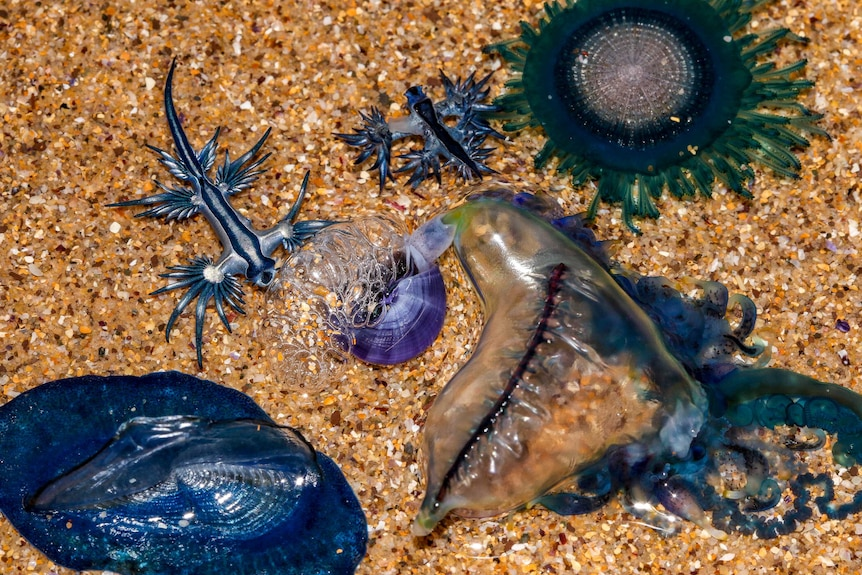
\includegraphics{./Images/BlueFleet_Image_ABC.jpeg}

\hypertarget{introduction}{%
\section{1. Introduction}\label{introduction}}

The blue fleet refers to a community of neustonic (i.e.~drifting or
floating with winds and currents) organisms, with a cosmopolitan
distribution (Bourg \emph{et al}., 2022). The community consists of
several species of Cnidaria (Jellyfish and relatives) as well as a
variety of Molluscs (Helm, 2021). Aggregations of these organisms may
cover extremely large areas, sometimes spanning several kilometers.
Whilst large fleets are generally confined to offshore areas, such as
oceanic gyres, strong onshore winds and currents can cause mass
strandings of these creatures (Bourg \emph{et al}., 2022). This poses a
risk to swimmers and beachgoers, as several constituent species possess
the ability to envenomate people or animals upon touch (e.g.~the
Bluebottle). The exact dynamics driving stranding of harmful species are
not completely understood, however this is an area of active research
(e.g.~Bourg \emph{et al}., 2022; Lee \emph{et al}., 2021).
Interestingly, there is some variability in the number of species that
one might find during a mass stranding event: sometimes we see all
species strand, whilst at other times only one species may be recorded
(Grove, 2010). This could be explained by the inherent morphological
differences between the species that make up the blue fleet. For
example, several cnidarians, including the bluebottle and the
by-the-wind sailor (\emph{Vellela vellela}), have evolved an enlarged
membrane filled with gas that serves as a sail. Individual bluebottles
come in a right or left-sailed orientation: these two morphotypes will
drift in opposite directions from each other (Bourg \emph{et al}., 2022;
Lee \emph{et al}., 2021). Other functional groups, such as the pelagic
slugs that prey on the floating cnidarians, lack such structures. Thus,
whilst all these species are considered part of the blue fleet, physical
forces might affect them in different ways.

Here, we simulate the drifting dynamics of two species that are part of
the blue fleet: The bluebottle \emph{Physalia physalis} (Cnidaria:
Siphonophora) and The `Blue Dragon' \emph{Glaucus atlanticus}
(Gastropoda: Nudibranchia), a pelagic sea slug and a predator of
\emph{P. physalis}. Drifting behaviour, and associated beaching
probabilities for each species were investigated through the use of an
Individual Based Model (IBM). We incorporate meaningful ecological
interactions between the two species, such as predation, to promote
realism of the drifting dynamics. Not much is known about how Blue
Dragons find their prey. However, it is possible that they are capable
of very limited directed movement, as well as chemodetection of nearby
prey using specialised structures known as rhinophores (Valdes \&
Compillo, 2004). Helm (2021) found that different species of pelagic
slugs had distinct unique predatory preferences and behaviours when
exposed to prey in a laboratory environment. Alternatively, prey density
might be so high that Blue Dragons simply rely on chance encounters with
prey. By simulating this system with different combinations of prey
densities and biological parameters, we aim to generate insights into
how a small neustonic predator finds prey.

We thus strive to answer the following questions:

\begin{enumerate}
\def\labelenumi{\arabic{enumi}.}
\item
  \emph{How do beaching probabilities differ between the two species?}
\item
  \emph{How do prey density, swimming speed and chemodetection affect
  the number of predator-prey interactions?}
\end{enumerate}

\hypertarget{model-elaboration}{%
\section{2. Model Elaboration}\label{model-elaboration}}

\hypertarget{conceptual-overview}{%
\subsection{2.1 Conceptual Overview}\label{conceptual-overview}}

The model is designed to investigate the effects of physical factors
such as wind and ocean currents on the movement and behavior of the two
species. We created a 100km x 10km grid, with a spatial resolution of 1
km (1,000 total cells). Cells with x-values \textgreater{} 1km were
assigned a `land' status and all other cells where assigned an `ocean'
status. This resulted in a straight coastline stretching the left side
of the grid, emulating a simplified Eastern Australian Coastline. Each
individual cell was then assigned a value for the following physical
parameters: Wind Speed, Wind Direction, Current Speed, Current
Direction. The temporal resolution was 1 hour. Thus, all speed
parameters are in km/H, and each simulation iteration represents 1 hour
in real-time.

The environment was then populated with individual \emph{G. atlanticus}
and \emph{P. physalis}, each with their own unique attributes. For
\emph{G. atlanticus}, we assigned the following attributes: initial X
coordinate, initial Y coordinate, chemodetection range, and movement
speed. As both chemodetection and speed are traits that are expected to
vary between \emph{G. atlanticus}, these were assigned by drawing from a
normal distribution with mean = 1 meter and sd = 0.25 meter for
chemodetection and mean = 0.15 cm/H and sd = 3.75 (proportion of sd to
mean was unchanged for simulations in which speed and chemodetection
were varied). There was no prior information available for these values,
so they are largely based on assumptions. Individual \emph{G.
atlanticus} could end up beached or alive at the end of the simulation.
For \emph{P. physalis}, the following attributes were assigned: initial
X coordinate, initial Y coordinate and orientation. Orientation refers
to the position of the sail relative to the tentacles: this comes in a
`right-handed' or `left-handed' variation. This variable was assigned
randomly for each individual. Individual \emph{P. physalis} could end up
beached, eaten, or alive at the end of the simulation.

Whilst the grid resolution was 1km, our model allows individuals to move
through continuous space. The movement of an individual depends on the
winds and current within the current cell, however the effect of these
drivers might only amount to a movement of 20 cm within a timestep. This
value is used to update the position of the individual. On the next
iteration, the individual will simply `feel' the same physical drivers,
as it still finds itself in the same cell. Thus, movement is decoupled
from grid cells, but the effect of wind and currents on the position of
an individual does depend on the grid cell they are in. This enables us
to include the biological interactions that occur on the scale of
centimeters.

\begin{itemize}
\tightlist
\item
  \textbf{\emph{Note: I initially opted for a grid approach as I was
  thinking about assigning distinct directions and speeds to different
  parts of the simulated environment. I did not end up doing this, so
  the grid structure is not really necessary, however I left it in as it
  makes no difference and allows me to maybe make those changes in a
  future version.}}
\end{itemize}

\hypertarget{movement-equations}{%
\subsection{2.2 Movement Equations}\label{movement-equations}}

\n

\hypertarget{glaucus-atlanticus}{%
\subsubsection{2.2.1 Glaucus atlanticus}\label{glaucus-atlanticus}}

\[
X_{j,i+1} = X_{ij} + 0.01 * WindSpeed_{{xy,i}} sin(WindDirection_{xy,i}) + 0.005 * CurrentSpeed_{xy,i} * sin(CurrentDirection_{xy,i}) + C * (GlaucusSpeed_{ij} * sin(atan(Y_{Prey} - Y_i, X_{Prey} - X_i)))
\] \[
Y_{j,i+1} = Y_{ij} + 0.01 * WindSpeed_{{xy,i}} * cos(WindDirection_{xy,i}) + 0.005 * CurrentSpeed_{xy,i} * cos(CurrentDirection_{xy,i}) + C * (GlaucusSpeed_{ij} * cos(atan(Y_{Prey} - Y_{ij}, X_{Prey} - X_{ij} )) )
\] \textbf{\emph{Where:}}

\[
X_{j,i+1} = \text{Position}\,\text{along}\,\text{the}\,\text{East-West}\,\text{Axis for}\,Individual_{j }\text{ at}\,\text{Time = }\,i+1 \\
X_{ij} = \text{Position}\,\text{along}\,\text{the}\,\text{East-West}\,\text{Axis for}\,Individual_{j }\text{ at}\,\text{Time = }\,i \\
Y_{j,i+1} = \text{Position}\,\text{along}\,\text{the}\,\text{North-South}\,\text{Axis for}\,Individual_{j }\text{ at}\,\text{Time = }\,i+1 \\
Y_{ij} = \text{Position}\,\text{along}\,\text{the}\,\text{North-South}\,\text{Axis for}\,Individual_{j }\text{ at}\,\text{Time = }\,i \\
WindSpeed_{xy,i} = \text{Wind Speed}\,\text{in}\, cell_{X_i,Y_i},\text{at}\,\text{Time = }\,i \\
WindDirection_{xy,i} = \text{Wind Direction}\,\text{in}\, cell_{X_i,Y_i},\text{at}\,\text{Time = }\,i \\
CurrentSpeed_{xy,i} = \text{Current Speed}\,\text{in}\, cell_{X_i,Y_i},\text{at}\,\text{Time = }\,i \\
CurrentDirection_{xy,i} = \text{Current Direction}\,\text{in}\, cell_{X_i,Y_i},\text{at}\,\text{Time = }\,i \\
GlaucusSpeed_{i,j} = \text{Swimming Speed}\,\text{for}\, Individual_{j }\text{ at}\,\text{Time = }\,i \\
Y_{prey} = \text{Y coordinate of closest prey for}\, Individual_{j } \text{ at Time = } i \\
X_{prey} = \text{X coordinate of closest prey for}\, Individual_{j } \text{ at Time = } i \\
Prey = ∀Physalia \\
C = \begin{cases}
1, & \text{if Prey within } Detection Range_j \\
0, & \text{if Prey beyond } Detection Range_j
\end{cases}
\]

The movement of \emph{G. atlanticus}s depends on physical and biological
parameters. For iteration i of the model, the position of an individual
is given by the x and y coordinate. The displacement between time = i
and time = i + 1 is given by above equations. The effects of winds and
current depend on i) the speed in km/h and ii) the direction in radians.
Sin(direction) then gives vertical (north-south) displacement, whilst
cos(direction) gives horizontal (east-west). To illustrate, if wind is
blowing from the east, direction equals 1.5 * pi. Displacement can then
be calculated as:

\[
\Delta_{x} = sin(1.5 * pi) * speed = -1*speed \\
\Delta_{y} = cos(1.5*pi) = 0 \\
\text{Thus, wind from the east will move an individual to the west}
\]

In addition, we allow \emph{G. atlanticus} to make small directed
movements towards prey, if their prey is within a certain `detection
zone'. The size of this detection zone depends on the chemodetection
abilities of an individual \emph{G. atlanticus}. If a prey item is
within the zone, we calculate the angle in radians between the predator
and the prey, and multiply this new direction by the speed of that
particular \emph{G. atlanticus}. The \emph{G. atlanticus} will always
move to the closest prey item it detects.

\begin{Shaded}
\begin{Highlighting}[]
\CommentTok{\# Movement of Glaucus: depends on an individual glaucus and the physalia fleet}
\NormalTok{glaucusMovement }\OtherTok{\textless{}{-}} \ControlFlowTok{function}\NormalTok{(glaucus, physalia)\{}
  
  \CommentTok{\# Boundary conditions for movement, i.e. out of frame.}
  \CommentTok{\# stop updating if this is the case}
  \ControlFlowTok{if}\NormalTok{(glaucus}\SpecialCharTok{$}\NormalTok{y }\SpecialCharTok{\textgreater{}=} \DecValTok{100} \SpecialCharTok{|}\NormalTok{ glaucus}\SpecialCharTok{$}\NormalTok{y }\SpecialCharTok{\textless{}=} \DecValTok{1} \SpecialCharTok{|}\NormalTok{ glaucus}\SpecialCharTok{$}\NormalTok{x }\SpecialCharTok{\textgreater{}=} \DecValTok{10}\NormalTok{)\{ }
    \FunctionTok{return}\NormalTok{(glaucus)\}}
  
  \CommentTok{\# First check if glaucus are \textquotesingle{}latched on\textquotesingle{} to physalia which will }
  \CommentTok{\# affect their movement. The physalia has to be alive.}
  \ControlFlowTok{if}\NormalTok{(}\SpecialCharTok{!}\FunctionTok{is.na}\NormalTok{(glaucus}\SpecialCharTok{$}\NormalTok{target\_ID) }\SpecialCharTok{\&}\NormalTok{ physalia[glaucus}\SpecialCharTok{$}\NormalTok{target\_ID,}\StringTok{\textquotesingle{}status\textquotesingle{}}\NormalTok{][}\DecValTok{1}\NormalTok{] }\SpecialCharTok{!=} \StringTok{\textquotesingle{}EATEN\textquotesingle{}}\NormalTok{)\{}
\NormalTok{    glaucus}\SpecialCharTok{$}\NormalTok{x }\OtherTok{\textless{}{-}}\NormalTok{ physalia[glaucus}\SpecialCharTok{$}\NormalTok{target\_ID,}\StringTok{\textquotesingle{}x\textquotesingle{}}\NormalTok{]}
\NormalTok{    glaucus}\SpecialCharTok{$}\NormalTok{y }\OtherTok{\textless{}{-}}\NormalTok{ physalia[glaucus}\SpecialCharTok{$}\NormalTok{target\_ID,}\StringTok{\textquotesingle{}y\textquotesingle{}}\NormalTok{]}
\NormalTok{    glaucus}\SpecialCharTok{$}\NormalTok{latch\_time }\OtherTok{\textless{}{-}}\NormalTok{ glaucus}\SpecialCharTok{$}\NormalTok{latch\_time }\SpecialCharTok{+} \DecValTok{1}
\NormalTok{    glaucus}\SpecialCharTok{$}\NormalTok{total\_latch\_time }\OtherTok{\textless{}{-}}\NormalTok{ glaucus}\SpecialCharTok{$}\NormalTok{total\_latch\_time }\SpecialCharTok{+} \DecValTok{1}
    
    \CommentTok{\# Probability of glaucus detaching follows a beta prime distribution.}
    \CommentTok{\# Shape of distribtution set to match expected behaviour {-} though arbitrary.}

\NormalTok{    probs }\OtherTok{\textless{}{-}} \FunctionTok{c}\NormalTok{(}\DecValTok{1}\SpecialCharTok{{-}}\FunctionTok{pbetapr}\NormalTok{(glaucus}\SpecialCharTok{$}\NormalTok{latch\_time, }\DecValTok{24}\NormalTok{, }\DecValTok{5}\NormalTok{), }\FunctionTok{pbetapr}\NormalTok{(glaucus}\SpecialCharTok{$}\NormalTok{latch\_time, }\DecValTok{24}\NormalTok{, }\DecValTok{5}\NormalTok{))}
\NormalTok{    glaucus}\SpecialCharTok{$}\NormalTok{target\_ID }\OtherTok{\textless{}{-}} \FunctionTok{sample}\NormalTok{(}\AttributeTok{size=}\DecValTok{1}\NormalTok{, }\AttributeTok{x =} \FunctionTok{c}\NormalTok{(glaucus}\SpecialCharTok{$}\NormalTok{target\_ID, }\ConstantTok{NA}\NormalTok{), }\AttributeTok{prob =}\NormalTok{ probs) }\CommentTok{\# NA corresponds to letting go of prey.}
    
\NormalTok{  \}}\ControlFlowTok{else}\NormalTok{\{}
    
    
    \CommentTok{\# Check the Glaucus is not beached, if OK, proceed with movement update}
    \CommentTok{\# as effect of physical forces}
    \ControlFlowTok{if}\NormalTok{(glaucus}\SpecialCharTok{$}\NormalTok{x }\SpecialCharTok{\textgreater{}} \DecValTok{1}\NormalTok{)\{}
   
      \CommentTok{\# Positional update rules: movement of a Glaucus}
      \CommentTok{\# We use ceiling() to round up and extract force values from the grids.}
      \CommentTok{\# The grids are set globally prior to function call.}
\NormalTok{      glaucus}\SpecialCharTok{$}\NormalTok{x }\OtherTok{\textless{}{-}}\NormalTok{ glaucus}\SpecialCharTok{$}\NormalTok{x }\SpecialCharTok{+} \FloatTok{0.01}\SpecialCharTok{*}\NormalTok{wind\_strength[}\FunctionTok{ceiling}\NormalTok{(glaucus}\SpecialCharTok{$}\NormalTok{y), }
                                                   \FunctionTok{ceiling}\NormalTok{(glaucus}\SpecialCharTok{$}\NormalTok{x)] }\SpecialCharTok{*} \FunctionTok{sin}\NormalTok{(wind\_direction[}\FunctionTok{ceiling}\NormalTok{(glaucus}\SpecialCharTok{$}\NormalTok{y), }
                                                                                            \FunctionTok{ceiling}\NormalTok{(glaucus}\SpecialCharTok{$}\NormalTok{x)])}\SpecialCharTok{+}
        \FloatTok{0.005} \SpecialCharTok{*}\NormalTok{ current\_strength[}\FunctionTok{ceiling}\NormalTok{(glaucus}\SpecialCharTok{$}\NormalTok{y), }
                                 \FunctionTok{ceiling}\NormalTok{(glaucus}\SpecialCharTok{$}\NormalTok{x)] }\SpecialCharTok{*} \FunctionTok{sin}\NormalTok{(current\_direction[}\FunctionTok{ceiling}\NormalTok{(glaucus}\SpecialCharTok{$}\NormalTok{y), }
                                                                             \FunctionTok{ceiling}\NormalTok{(glaucus}\SpecialCharTok{$}\NormalTok{x)])}
      
      \CommentTok{\# Y movement (north {-} south) uses cosine function}
\NormalTok{      glaucus}\SpecialCharTok{$}\NormalTok{y }\OtherTok{\textless{}{-}}\NormalTok{ glaucus}\SpecialCharTok{$}\NormalTok{y }\SpecialCharTok{+} \FloatTok{0.01}\SpecialCharTok{*}\NormalTok{wind\_strength[}\FunctionTok{ceiling}\NormalTok{(glaucus}\SpecialCharTok{$}\NormalTok{y), }
                                                   \FunctionTok{ceiling}\NormalTok{(glaucus}\SpecialCharTok{$}\NormalTok{x)] }\SpecialCharTok{*} \FunctionTok{cos}\NormalTok{(wind\_direction[}\FunctionTok{ceiling}\NormalTok{(glaucus}\SpecialCharTok{$}\NormalTok{y), }
                                                                                            \FunctionTok{ceiling}\NormalTok{(glaucus}\SpecialCharTok{$}\NormalTok{x)]) }\SpecialCharTok{+}
        \FloatTok{0.005} \SpecialCharTok{*}\NormalTok{ current\_strength[}\FunctionTok{ceiling}\NormalTok{(glaucus}\SpecialCharTok{$}\NormalTok{y), }
                                 \FunctionTok{ceiling}\NormalTok{(glaucus}\SpecialCharTok{$}\NormalTok{x)] }\SpecialCharTok{*} \FunctionTok{cos}\NormalTok{(current\_direction[}\FunctionTok{ceiling}\NormalTok{(glaucus}\SpecialCharTok{$}\NormalTok{y), }
                                                                             \FunctionTok{ceiling}\NormalTok{(glaucus}\SpecialCharTok{$}\NormalTok{x)])}
      
      \DocumentationTok{\#\#\# Predator module {-} handles the predator behaviour}
      
      \CommentTok{\# Glaucus are predators. They can detect prey from distance using chemical cues. We want to simulate these capabilities}
      \CommentTok{\# by allowing glaucus limited movement to a target, if the target is within reasonable range.}
      
      \CommentTok{\# scan area for each glaucus}
      \CommentTok{\# Convert to spatial geometries to allow geometric operations.}
\NormalTok{      spat.point }\OtherTok{\textless{}{-}} \FunctionTok{st\_point}\NormalTok{(}\FunctionTok{c}\NormalTok{(glaucus}\SpecialCharTok{$}\NormalTok{x, glaucus}\SpecialCharTok{$}\NormalTok{y))}
      
      \CommentTok{\# Chemodetection range calculated as circle with radius equal to }
      \CommentTok{\# the predetermined parameter.}
\NormalTok{      detection.zone }\OtherTok{\textless{}{-}} \FunctionTok{st\_buffer}\NormalTok{(spat.point, glaucus}\SpecialCharTok{$}\NormalTok{chemodetection)}
      
      \CommentTok{\# Find the Physalia that are within the detection zone.}
\NormalTok{      physalia.df.spat }\OtherTok{\textless{}{-}} \FunctionTok{st\_as\_sf}\NormalTok{(physalia , }\AttributeTok{coords =} \FunctionTok{c}\NormalTok{(}\StringTok{\textquotesingle{}x\textquotesingle{}}\NormalTok{, }\StringTok{\textquotesingle{}y\textquotesingle{}}\NormalTok{))}
      
      \CommentTok{\# Any prey in the detection zone?}
      \ControlFlowTok{if}\NormalTok{(}\FunctionTok{any}\NormalTok{(}\FunctionTok{st\_intersects}\NormalTok{(physalia.df.spat, detection.zone, }\AttributeTok{sparse =}\NormalTok{ F)))\{}
        \CommentTok{\# Find the nearest Physalia}
        \FunctionTok{print}\NormalTok{(}\StringTok{\textquotesingle{}Attack!\textquotesingle{}}\NormalTok{) }\CommentTok{\# to check if all is ok}
        
        \CommentTok{\# extract some info on the prey}
\NormalTok{        glaucus.target }\OtherTok{\textless{}{-}}\NormalTok{ physalia.df.spat[[}\FunctionTok{which.min}\NormalTok{(}\FunctionTok{st\_distance}\NormalTok{(spat.point, physalia.df.spat)),}\StringTok{\textquotesingle{}geometry\textquotesingle{}}\NormalTok{]]}
\NormalTok{        glaucus.target.id }\OtherTok{\textless{}{-}}\NormalTok{ physalia.df.spat[[}\FunctionTok{which.min}\NormalTok{(}\FunctionTok{st\_distance}\NormalTok{(spat.point, physalia.df.spat)),}\StringTok{\textquotesingle{}ID\textquotesingle{}}\NormalTok{]]}
        
        \CommentTok{\# Now make it move towards the target. We just assume it }
        \CommentTok{\# is quite good at sensing prey so its movement is }
        \CommentTok{\# directed.}
        
\NormalTok{        target\_angle }\OtherTok{\textless{}{-}} \FunctionTok{atan2}\NormalTok{(glaucus.target[}\DecValTok{2}\NormalTok{] }\SpecialCharTok{{-}}\NormalTok{ glaucus}\SpecialCharTok{$}\NormalTok{y, glaucus.target[}\DecValTok{1}\NormalTok{] }\SpecialCharTok{{-}}\NormalTok{ glaucus}\SpecialCharTok{$}\NormalTok{x) }\CommentTok{\# atan2 calculates the angle to get from y to x}
\NormalTok{        glaucus}\SpecialCharTok{$}\NormalTok{x }\OtherTok{\textless{}{-}}\NormalTok{ glaucus}\SpecialCharTok{$}\NormalTok{x }\SpecialCharTok{+}\NormalTok{ glaucus}\SpecialCharTok{$}\NormalTok{speed }\SpecialCharTok{*} \FunctionTok{cos}\NormalTok{(target\_angle) }
\NormalTok{        glaucus}\SpecialCharTok{$}\NormalTok{y }\OtherTok{\textless{}{-}}\NormalTok{ glaucus}\SpecialCharTok{$}\NormalTok{y }\SpecialCharTok{+}\NormalTok{  glaucus}\SpecialCharTok{$}\NormalTok{speed }\SpecialCharTok{*} \FunctionTok{sin}\NormalTok{(target\_angle)}
        
        \CommentTok{\# track interaction {-} defined as entities being close enough to change behaviour }
        \CommentTok{\# i.e. sensing, eating, latching}
\NormalTok{        glaucus}\SpecialCharTok{$}\NormalTok{interaction }\OtherTok{\textless{}{-}} \FunctionTok{as.numeric}\NormalTok{(glaucus}\SpecialCharTok{$}\NormalTok{interaction) }\SpecialCharTok{+} \DecValTok{1}
        
        \CommentTok{\# Latch{-}on module}
\NormalTok{        eating.zone }\OtherTok{\textless{}{-}} \FunctionTok{st\_buffer}\NormalTok{(spat.point, }\FloatTok{0.0005}\NormalTok{) }
        \ControlFlowTok{if}\NormalTok{(}\FunctionTok{st\_intersects}\NormalTok{(physalia.df.spat[glaucus.target.id,], eating.zone, }\AttributeTok{sparse =}\NormalTok{ F))\{}
          \FunctionTok{print}\NormalTok{(}\StringTok{\textquotesingle{}LATCHED\textquotesingle{}}\NormalTok{)}
          
          \CommentTok{\# Identify the prey to latch on and store as glaucus attribute}
\NormalTok{          glaucus}\SpecialCharTok{$}\NormalTok{target\_ID }\OtherTok{\textless{}{-}}\NormalTok{ glaucus.target.id }
          
\NormalTok{        \}}
\NormalTok{      \}}
      
      
\NormalTok{    \} }\ControlFlowTok{else}\NormalTok{\{}
\NormalTok{      glaucus}\SpecialCharTok{$}\NormalTok{status }\OtherTok{\textless{}{-}} \StringTok{\textquotesingle{}BEACHED\textquotesingle{}} \CommentTok{\# glaucus is beached}
\NormalTok{    \}}
\NormalTok{  \}}
  \FunctionTok{return}\NormalTok{(glaucus)}
\NormalTok{\}}
\end{Highlighting}
\end{Shaded}

\hypertarget{physalia-physalis}{%
\subsubsection{2.2.2 Physalia physalis}\label{physalia-physalis}}

\[
X_{j,i+1} = X_{ij} + 0.0266*(WindSpeed_{{xy,i}} * sin(WindDirection_{xy,i}+ D_{ij})) + 0.001 *CurrentSpeed_{xy,i} * sin(CurrentDirection_{xy,i}) \\
Y_{j,i+1} = Y_{ij} + 0.0266*(WindSpeed_{{xy,i}} * cos(WindDirection_{xy,i}+ D_{ij})) + 0.001 * CurrentSpeed_{xy,i} * cos(CurrentDirection_{xy,i})
\]

\textbf{\emph{Where:}}

\[
X_{j,i+1} = \text{Position}\,\text{along}\,\text{the}\,\text{East-West}\,\text{Axis for}\,Individual_{j }\text{ at}\,\text{Time = }\,i+1 \\
X_{ij} = \text{Position}\,\text{along}\,\text{the}\,\text{East-West}\,\text{Axis for}\,Individual_{j }\text{ at}\,\text{Time = }\,i \\
Y_{j,i+1} = \text{Position}\,\text{along}\,\text{the}\,\text{North-South}\,\text{Axis for}\,Individual_{j }\text{ at}\,\text{Time = }\,i+1 \\
Y_{ij} = \text{Position}\,\text{along}\,\text{the}\,\text{North-South}\,\text{Axis for}\,Individual_{j }\text{ at}\,\text{Time = }\,i \\
WindSpeed_{xy,i} = \text{Wind Speed}\,\text{in}\, cell_{X_i,Y_i},\text{at}\,\text{Time = }\,i \\
WindDirection_{xy,i} = \text{Wind Direction}\,\text{in}\, cell_{X_i,Y_i},\text{at}\,\text{Time = }\,i \\
CurrentSpeed_{xy,i} = \text{Current Speed}\,\text{in}\, cell_{X_i,Y_i},\text{at}\,\text{Time = }\,i \\
CurrentDirection_{xy,i} = \text{Current Direction}\,\text{in}\, cell_{X_i,Y_i},\text{at}\,\text{Time = }\,i \\
D_{ij} = \begin{cases}
normal(pi/3, 0.25) & \text{if Orientation}_j = Right \\
normal(-pi/3,0.25) & \text{if Orientation}_j = Left
\end{cases} \text{at Time = } i \\
Orientation_j = \text{Sail Orientation of Individual}_j \text{ at Time = } i
\]

\emph{P. physalis} moves at \textasciitilde2.66\% the speed of the wind
(Lee \emph{et al}., 2021). Left-sailed individuals will be pushed in a
direction 50 degrees to the left of the prevailing wind, whilst right
handed individuals move 50 degrees to the right of prevailing winds
(Bourg \emph{et al}., 2022). The effect of currents on \emph{P.
physalis} is then described using similar equations as for Glaucus.

\begin{Shaded}
\begin{Highlighting}[]
\CommentTok{\# Movement of Physalia}
\NormalTok{physaliaMovement }\OtherTok{\textless{}{-}} \ControlFlowTok{function}\NormalTok{(physalia, glaucus)\{}
  
  \CommentTok{\# Boundary conditions for movement, i.e. out of frame}
  \CommentTok{\# stop updating if this happens}
  \ControlFlowTok{if}\NormalTok{(physalia}\SpecialCharTok{$}\NormalTok{y }\SpecialCharTok{\textgreater{}=} \DecValTok{100} \SpecialCharTok{|}\NormalTok{ physalia}\SpecialCharTok{$}\NormalTok{y }\SpecialCharTok{\textless{}=} \DecValTok{1} \SpecialCharTok{|}\NormalTok{physalia}\SpecialCharTok{$}\NormalTok{x }\SpecialCharTok{\textgreater{}=} \DecValTok{100}\NormalTok{)\{}
    
    \FunctionTok{return}\NormalTok{(physalia)\}}

  \CommentTok{\# Check Physalia is alive and not beached}
  \ControlFlowTok{if}\NormalTok{(physalia}\SpecialCharTok{$}\NormalTok{x }\SpecialCharTok{\textgreater{}} \DecValTok{1} \SpecialCharTok{\&}\NormalTok{ physalia}\SpecialCharTok{$}\NormalTok{status }\SpecialCharTok{!=} \StringTok{\textquotesingle{}EATEN\textquotesingle{}}\NormalTok{)\{}
    
    \DocumentationTok{\#\#\# Predator{-}prey module}
    
    \CommentTok{\# We want to simulate damage to the physalia, i.e. being killed by a predator.}
    \CommentTok{\# We use a simple rule: if the glaucus is within feeding range of the physalia}
    \CommentTok{\# for 24 hours, the physalia has been eaten completely. The glaucus will then also}
    \CommentTok{\# move on as we assign status \textquotesingle{}eaten\textquotesingle{} to the physalia. }
    
    \CommentTok{\# Convert to spatial geometries to allow geometric operations.}
\NormalTok{    spat.point }\OtherTok{\textless{}{-}} \FunctionTok{st\_point}\NormalTok{(}\FunctionTok{c}\NormalTok{(physalia}\SpecialCharTok{$}\NormalTok{x, physalia}\SpecialCharTok{$}\NormalTok{y))}
    
    \CommentTok{\# We can decide what a reasonable buffer is. This is the same for}
    \CommentTok{\# all physalia. }
\NormalTok{    under.attack.zone }\OtherTok{\textless{}{-}} \FunctionTok{st\_buffer}\NormalTok{(spat.point, }\FloatTok{0.0005}\NormalTok{)}
    
    \CommentTok{\# Check if there is a predator nearby}
\NormalTok{    glaucus.df.spat }\OtherTok{\textless{}{-}} \FunctionTok{st\_as\_sf}\NormalTok{(glaucus , }\AttributeTok{coords =} \FunctionTok{c}\NormalTok{(}\StringTok{\textquotesingle{}x\textquotesingle{}}\NormalTok{, }\StringTok{\textquotesingle{}y\textquotesingle{}}\NormalTok{))}
    
    \CommentTok{\# Any predators in the detection/eating zone?}
    \ControlFlowTok{if}\NormalTok{(}\FunctionTok{any}\NormalTok{(}\FunctionTok{st\_intersects}\NormalTok{(glaucus.df.spat, under.attack.zone, }\AttributeTok{sparse =}\NormalTok{ F)))\{}
      
      \CommentTok{\# If yes, the physalia is \textquotesingle{}under attack\textquotesingle{}}
\NormalTok{      physalia}\SpecialCharTok{$}\NormalTok{underattack }\OtherTok{\textless{}{-}}\NormalTok{ physalia}\SpecialCharTok{$}\NormalTok{underattack }\SpecialCharTok{+} \DecValTok{1}
\NormalTok{    \}}
    \CommentTok{\# Check if physalia is eaten }
    \ControlFlowTok{if}\NormalTok{(physalia}\SpecialCharTok{$}\NormalTok{underattack }\SpecialCharTok{\textgreater{}=} \DecValTok{24}\NormalTok{)\{}
\NormalTok{      physalia}\SpecialCharTok{$}\NormalTok{status }\OtherTok{\textless{}{-}} \StringTok{\textquotesingle{}EATEN\textquotesingle{}}
\NormalTok{    \}}
    
    \CommentTok{\# We have right and left=handed bluebottles}
    \CommentTok{\# They drift in opposite directions {-} presumably to sustain populations.}
    \CommentTok{\# We need to account for this properly. In addition, we want to add some}
    \CommentTok{\# stochasticity to the movement. This is due to inherent variability}
    \CommentTok{\# in the shape and size of bluebottles, but also due to waves etc.}
    
    \ControlFlowTok{if}\NormalTok{(physalia}\SpecialCharTok{$}\NormalTok{orientation }\SpecialCharTok{==} \StringTok{\textquotesingle{}right\textquotesingle{}}\NormalTok{) \{direction\_offset }\OtherTok{\textless{}{-}} \FunctionTok{rnorm}\NormalTok{(}\DecValTok{1}\NormalTok{,}\DecValTok{1}\NormalTok{,}\FloatTok{0.25}\NormalTok{)}\SpecialCharTok{*}\NormalTok{pi}\SpecialCharTok{/}\DecValTok{3}\NormalTok{\} }\CommentTok{\# right{-}handed drift at 50 degrees from wind direction.}
    \ControlFlowTok{if}\NormalTok{(physalia}\SpecialCharTok{$}\NormalTok{orientation }\SpecialCharTok{==} \StringTok{\textquotesingle{}left\textquotesingle{}}\NormalTok{) \{direction\_offset }\OtherTok{\textless{}{-}} \FunctionTok{rnorm}\NormalTok{(}\DecValTok{1}\NormalTok{,}\SpecialCharTok{{-}}\DecValTok{1}\NormalTok{,}\FloatTok{0.25}\NormalTok{)}\SpecialCharTok{*}\NormalTok{pi}\SpecialCharTok{/}\DecValTok{3}\NormalTok{\} }\CommentTok{\# left handed drift at \textasciigrave{}\textasciigrave{}}
    
    \CommentTok{\# Positional update rules:}
    \CommentTok{\# Wind has a larger impact on physalia due to the sail}
    \CommentTok{\# physalia also have an offset {-} their sails change the way they interact with wind. }
    \CommentTok{\# We also assume current has a slightly smaller effect on them than on glaucus}

    \CommentTok{\# 0.0266 {-} see Lee, Schaeffer, Groeskamp (2021) for justification.}
\NormalTok{    physalia}\SpecialCharTok{$}\NormalTok{x }\OtherTok{\textless{}{-}}\NormalTok{ physalia}\SpecialCharTok{$}\NormalTok{x }\SpecialCharTok{+} \FloatTok{0.0266}\SpecialCharTok{*}\NormalTok{(wind\_strength[}\FunctionTok{ceiling}\NormalTok{(physalia}\SpecialCharTok{$}\NormalTok{y), }
                                                     \FunctionTok{ceiling}\NormalTok{(physalia}\SpecialCharTok{$}\NormalTok{x)]) }\SpecialCharTok{*} \FunctionTok{sin}\NormalTok{(wind\_direction[}\FunctionTok{ceiling}\NormalTok{(physalia}\SpecialCharTok{$}\NormalTok{y), }
                                                                                                          \FunctionTok{ceiling}\NormalTok{(physalia}\SpecialCharTok{$}\NormalTok{x)]}\SpecialCharTok{+}\NormalTok{ direction\_offset) }\SpecialCharTok{+}
      \FloatTok{0.001}\SpecialCharTok{*}\NormalTok{ current\_strength[}\FunctionTok{ceiling}\NormalTok{(physalia}\SpecialCharTok{$}\NormalTok{y), }
                              \FunctionTok{ceiling}\NormalTok{(physalia}\SpecialCharTok{$}\NormalTok{x)] }\SpecialCharTok{*} \FunctionTok{sin}\NormalTok{(current\_direction[}\FunctionTok{ceiling}\NormalTok{(physalia}\SpecialCharTok{$}\NormalTok{y), }
                                                                                     \FunctionTok{ceiling}\NormalTok{(physalia}\SpecialCharTok{$}\NormalTok{x)])}
    
    \CommentTok{\# Y movement (north {-} south) uses cosine function}
\NormalTok{    physalia}\SpecialCharTok{$}\NormalTok{y }\OtherTok{\textless{}{-}}\NormalTok{ physalia}\SpecialCharTok{$}\NormalTok{y }\SpecialCharTok{+} \FloatTok{0.0266}\SpecialCharTok{*}\NormalTok{(wind\_strength[}\FunctionTok{ceiling}\NormalTok{(physalia}\SpecialCharTok{$}\NormalTok{y), }
                                                     \FunctionTok{ceiling}\NormalTok{(physalia}\SpecialCharTok{$}\NormalTok{x)]) }\SpecialCharTok{*} \FunctionTok{cos}\NormalTok{(wind\_direction[}\FunctionTok{ceiling}\NormalTok{(physalia}\SpecialCharTok{$}\NormalTok{y), }
                                                                                                          \FunctionTok{ceiling}\NormalTok{(physalia}\SpecialCharTok{$}\NormalTok{x)] }\SpecialCharTok{+}\NormalTok{ direction\_offset) }\SpecialCharTok{+}
      \FloatTok{0.001}\SpecialCharTok{*}\NormalTok{ current\_strength[}\FunctionTok{ceiling}\NormalTok{(physalia}\SpecialCharTok{$}\NormalTok{y), }
                              \FunctionTok{ceiling}\NormalTok{(physalia}\SpecialCharTok{$}\NormalTok{x)] }\SpecialCharTok{*} \FunctionTok{cos}\NormalTok{(current\_direction[}\FunctionTok{ceiling}\NormalTok{(physalia}\SpecialCharTok{$}\NormalTok{y), }
                                                                                     \FunctionTok{ceiling}\NormalTok{(physalia}\SpecialCharTok{$}\NormalTok{x)])}
    
\NormalTok{  \} }\ControlFlowTok{else}\NormalTok{\{}
  
    \CommentTok{\# Check if individual is beached}
    \ControlFlowTok{if}\NormalTok{(physalia}\SpecialCharTok{$}\NormalTok{x }\SpecialCharTok{\textless{}=} \DecValTok{1}\NormalTok{)\{}
\NormalTok{      physalia}\SpecialCharTok{$}\NormalTok{status }\OtherTok{\textless{}{-}} \StringTok{\textquotesingle{}BEACHED\textquotesingle{}}
\NormalTok{    \}}
\NormalTok{  \}}
  \FunctionTok{return}\NormalTok{(physalia)}
\NormalTok{\}}
\end{Highlighting}
\end{Shaded}

\hypertarget{biological-interactions}{%
\subsubsection{2.3 Biological
Interactions}\label{biological-interactions}}

Both species are able to interact with each other in the model, and this
potentially affects their movements. \emph{G. atlanticus} will seek out
nearby \emph{P. physalis} as described in section 2.2.1. However, they
may also `latch' on to a \emph{P. physalis}. This emulates feeding
behaviour in which \emph{G. atlanticus} move within the tentacles of a
\emph{P. physalis}: \emph{G. atlanticus} may then move with the \emph{P.
physalis}, until it stops feeding or completely depletes the resource.
Consequently, the time it takes to deplete the resource equals the time
it takes for a \emph{P. physalis} to be killed. We assume that an
individual \emph{P. physalis} cannot survive unlimited attacks by
\emph{G. atlanticus}, and thus an individual that spends more than 24
hours `under attack' will be assigned the status `EATEN' and no further
movements are simulated. Any \emph{G. atlanticus} that was `latched on'
to the deceased prey, or one that simply stops feeding, then reverts to
their regular movement equations. Individual \emph{G. atlanticus} may
also detach from prey before consuming it. We model detachment using a
beta prime distribution (α = 24, β = 5), by letting the probability of
detaching equal the probability of observing a given latch time from the
specified beta prime distribution.

\hypertarget{stochasticity-of-winds-and-currents}{%
\subsubsection{2.4 Stochasticity of Winds and
Currents}\label{stochasticity-of-winds-and-currents}}

We strived to emulate the wind and current regime of the East Australian
coastline. The primary current is the EAC, which flows in a southward
direction. The current speed was initialized at a 5 km/H; this was
deemed reasonable as the top speed of the EAC is thought to be around 7
km/H (XXX). We then allowed speeds to increase or decrease
stochastically, within a range of 2 km/H - 7 km/H. Wind and current
direction were initialized at 315° and 180° and allowed to vary: wind
direction varies between 225° and 315°, whilst current direction varies
between 160° and 200°. This approach directions did not `jump' randomly,
but instead changed due to small stochastic increases or decreases.
These ranges were based on available data (WillyWeather, 2023; Middleton
\emph{et al}., 1996).

Wind speed was modeled following a slightly different approach. Wind
speed generally follows a daily cycle, in which wind builds up
throughout the day. We simulated this using a sine function with added
gaussian noise - this function is featured in the following code chunk.

\begin{Shaded}
\begin{Highlighting}[]
\CommentTok{\# Stochastic parameter wind strength}
\NormalTok{wind\_strength\_calc }\OtherTok{\textless{}{-}}\ControlFlowTok{function}\NormalTok{(hour) \{}
  \CommentTok{\# Parameters for the sinusoidal function}
\NormalTok{  peak\_hour }\OtherTok{\textless{}{-}} \DecValTok{20}        \CommentTok{\# Hour of the day with maximum wind}
\NormalTok{  amplitude }\OtherTok{\textless{}{-}} \DecValTok{5}       \CommentTok{\# Amplitude of the sinusoidal function (half of the variation)}
  
  
  \CommentTok{\# Calculate daylight hours using a sinusoidal function}
\NormalTok{  strength }\OtherTok{=}\NormalTok{ amplitude }\SpecialCharTok{*} \FunctionTok{sin}\NormalTok{((hour }\SpecialCharTok{{-}}\NormalTok{ peak\_hour) }\SpecialCharTok{*} \DecValTok{2} \SpecialCharTok{*}\NormalTok{ pi }\SpecialCharTok{/} \DecValTok{24}\NormalTok{) }\SpecialCharTok{+} \DecValTok{10} 
\NormalTok{  strength }\OtherTok{=}\NormalTok{ (strength }\SpecialCharTok{+} \FunctionTok{rnorm}\NormalTok{(}\FunctionTok{length}\NormalTok{(hour), }\DecValTok{0}\NormalTok{, }\AttributeTok{sd =} \DecValTok{3}\NormalTok{))}
\NormalTok{  strength[}\FunctionTok{which}\NormalTok{(strength}\SpecialCharTok{\textless{}}\DecValTok{0}\NormalTok{)] }\OtherTok{\textless{}{-}} \DecValTok{0}
  \FunctionTok{return}\NormalTok{(strength)}
\NormalTok{\}}
\end{Highlighting}
\end{Shaded}

\hypertarget{model-simulations}{%
\section{3. Model Simulations}\label{model-simulations}}

In order to effectively answer our research questions, we designed a
simulation strategy consisting of two distinct parts: i) running 32
replicates of the simulation using fixed behavioral parameters and
assessing beaching proportions of each species and ii) running 50
simulations, each with a different combination of chemodetection range
and swimming speed between 0 and 20 meters, obtained from a Latin Square
Sampling design, at three different densities of \emph{P. physalis} (a
total of 150 unique simulations). All simulations were run on a HPC
cluster - bash scripts used are included in the appendix.

\hypertarget{simulation-function}{%
\subsection{3.1 Simulation Function}\label{simulation-function}}

We created a main simulation function that handles creation of the
environment, instantiation of agents, and movement updates based on a
fixed number of hours or iterations. The function takes 10 parameters to
achieve this.

\begin{Shaded}
\begin{Highlighting}[]
\CommentTok{\# Function for running simulation }
\NormalTok{simBlueFleet.stochPhys }\OtherTok{\textless{}{-}} \ControlFlowTok{function}\NormalTok{(nTimes,n\_rows, n\_cols, nPhysalia, nGlaucus,}
\NormalTok{                                   strength\_current,}
\NormalTok{                                   dir\_wind, dir\_current,}
\NormalTok{                                   glaucus\_Chemodetection, glaucus\_Speed, iniSpace)\{}
  
  \CommentTok{\# Assign wind and current speed and direction to each grid cell.}
  \CommentTok{\# Based on param input}
\NormalTok{  current\_strength }\OtherTok{\textless{}\textless{}{-}} \FunctionTok{matrix}\NormalTok{(}\FunctionTok{rep}\NormalTok{(strength\_current,n\_rows}\SpecialCharTok{*}\NormalTok{n\_cols), }
                              \AttributeTok{nrow=}\NormalTok{n\_rows)}
  
  \CommentTok{\# Wind and current directions}
  
\NormalTok{  wind\_direction }\OtherTok{\textless{}\textless{}{-}} \FunctionTok{matrix}\NormalTok{(}\FunctionTok{rep}\NormalTok{(dir\_wind, n\_rows}\SpecialCharTok{*}\NormalTok{n\_cols), }
                            \AttributeTok{nrow=}\NormalTok{n\_rows, }\AttributeTok{ncol=}\NormalTok{n\_cols)}
\NormalTok{  current\_direction }\OtherTok{\textless{}\textless{}{-}} \FunctionTok{matrix}\NormalTok{(}\FunctionTok{rep}\NormalTok{(dir\_current, n\_rows}\SpecialCharTok{*}\NormalTok{n\_cols), }
                               \AttributeTok{nrow=}\NormalTok{n\_rows, }\AttributeTok{ncol=}\NormalTok{n\_cols)}
  
  
  \DocumentationTok{\#\#\# Instantiate model agents}
  
  \CommentTok{\# Glaucus atlanticus individuals}
  \FunctionTok{print}\NormalTok{(}\StringTok{\textquotesingle{}Generating animals\textquotesingle{}}\NormalTok{)}
  \CommentTok{\# Our individuals also have attributes. Glaucus are our predators.}
  \CommentTok{\# They will seek out Physalia, and are capable of (very limited)}
  \CommentTok{\# powered movement. }
  
\NormalTok{  glaucus }\OtherTok{\textless{}{-}} \FunctionTok{data.frame}\NormalTok{(}\FunctionTok{matrix}\NormalTok{(}\AttributeTok{nrow=}\NormalTok{nGlaucus, }\AttributeTok{ncol=}\DecValTok{10}\NormalTok{))}
  \FunctionTok{colnames}\NormalTok{(glaucus) }\OtherTok{\textless{}{-}} \FunctionTok{c}\NormalTok{(}\StringTok{"ID"}\NormalTok{, }\StringTok{"x"}\NormalTok{, }\StringTok{"y"}\NormalTok{, }\StringTok{"chemodetection"}\NormalTok{, }\StringTok{"speed"}\NormalTok{, }\StringTok{"latch\_time"}\NormalTok{,}\StringTok{"total\_latch\_time"}\NormalTok{, }\StringTok{"target\_ID"}\NormalTok{, }\StringTok{"interaction"}\NormalTok{, }\StringTok{"status"}\NormalTok{)}
  \ControlFlowTok{for}\NormalTok{ (i }\ControlFlowTok{in} \DecValTok{1}\SpecialCharTok{:}\NormalTok{nGlaucus) \{}
\NormalTok{    glaucus[i,] }\OtherTok{\textless{}{-}} \FunctionTok{list}\NormalTok{(}
      \AttributeTok{ID =}\NormalTok{ i,}
      \AttributeTok{x =} \FunctionTok{round}\NormalTok{(}\FunctionTok{runif}\NormalTok{(}\DecValTok{1}\NormalTok{, iniSpace}\SpecialCharTok{$}\NormalTok{xmin, iniSpace}\SpecialCharTok{$}\NormalTok{xmax),}\DecValTok{3}\NormalTok{),}
      \AttributeTok{y =} \FunctionTok{round}\NormalTok{(}\FunctionTok{runif}\NormalTok{(}\DecValTok{1}\NormalTok{, iniSpace}\SpecialCharTok{$}\NormalTok{ymin, iniSpace}\SpecialCharTok{$}\NormalTok{ymax),}\DecValTok{3}\NormalTok{),}
      \AttributeTok{chemodetection =} \FunctionTok{rnorm}\NormalTok{(}\DecValTok{1}\NormalTok{, glaucus\_Chemodetection, glaucus\_Chemodetection}\SpecialCharTok{/}\DecValTok{4}\NormalTok{), }
      \AttributeTok{speed =} \FunctionTok{rnorm}\NormalTok{(}\DecValTok{1}\NormalTok{,glaucus\_Speed, }\AttributeTok{sd =}\NormalTok{ glaucus\_Speed}\SpecialCharTok{/}\DecValTok{4}\NormalTok{),}
      \AttributeTok{latch\_time =} \DecValTok{0}\NormalTok{,}
      \AttributeTok{total\_latch\_time =} \DecValTok{0}\NormalTok{,}
      \AttributeTok{target\_ID =} \ConstantTok{NA}\NormalTok{,}
      \AttributeTok{interaction =} \DecValTok{0}\NormalTok{,}
      \AttributeTok{status =} \StringTok{\textquotesingle{}ALIVE\textquotesingle{}}
\NormalTok{    )}
\NormalTok{  \}}
  
  \CommentTok{\# Set up bluebottle movement and functions. Bluebottles can be right}
  \CommentTok{\# or left handed.}
\NormalTok{  physalia }\OtherTok{\textless{}{-}} \FunctionTok{data.frame}\NormalTok{(}\FunctionTok{matrix}\NormalTok{(}\AttributeTok{nrow=}\NormalTok{nPhysalia, }\AttributeTok{ncol=}\DecValTok{6}\NormalTok{))}
  \FunctionTok{colnames}\NormalTok{(physalia) }\OtherTok{\textless{}{-}} \FunctionTok{c}\NormalTok{(}\StringTok{"ID"}\NormalTok{, }\StringTok{"x"}\NormalTok{, }\StringTok{"y"}\NormalTok{, }\StringTok{"underattack"}\NormalTok{, }\StringTok{"status"}\NormalTok{, }\StringTok{"orientation"}\NormalTok{)}
  
  \ControlFlowTok{for}\NormalTok{ (i }\ControlFlowTok{in} \DecValTok{1}\SpecialCharTok{:}\NormalTok{nPhysalia) \{}
\NormalTok{    physalia[i,] }\OtherTok{\textless{}{-}} \FunctionTok{list}\NormalTok{(}
      \AttributeTok{ID =}\NormalTok{ i,}
      \AttributeTok{x =} \FunctionTok{round}\NormalTok{(}\FunctionTok{runif}\NormalTok{(}\DecValTok{1}\NormalTok{, iniSpace}\SpecialCharTok{$}\NormalTok{xmin, iniSpace}\SpecialCharTok{$}\NormalTok{xmax),}\DecValTok{3}\NormalTok{),}
      \AttributeTok{y =} \FunctionTok{round}\NormalTok{(}\FunctionTok{runif}\NormalTok{(}\DecValTok{1}\NormalTok{, iniSpace}\SpecialCharTok{$}\NormalTok{ymin, iniSpace}\SpecialCharTok{$}\NormalTok{ymax),}\DecValTok{3}\NormalTok{),}
      \AttributeTok{underattack =} \DecValTok{0}\NormalTok{,}
      \AttributeTok{status =} \StringTok{\textquotesingle{}ALIVE\textquotesingle{}}\NormalTok{,}
      \AttributeTok{orientation =} \FunctionTok{sample}\NormalTok{(}\FunctionTok{c}\NormalTok{(}\StringTok{\textquotesingle{}left\textquotesingle{}}\NormalTok{, }\StringTok{\textquotesingle{}right\textquotesingle{}}\NormalTok{),}\DecValTok{1}\NormalTok{)}
\NormalTok{    )}
\NormalTok{  \}}
  
  \FunctionTok{print}\NormalTok{(}\StringTok{\textquotesingle{}Simulating Dynamics\textquotesingle{}}\NormalTok{)}
\NormalTok{  GlaucusSim }\OtherTok{\textless{}{-}} \FunctionTok{list}\NormalTok{()}
\NormalTok{  PhysaliaSim }\OtherTok{\textless{}{-}} \FunctionTok{list}\NormalTok{()}
  
  \CommentTok{\# Run model over nTimes steps.}
  \ControlFlowTok{for}\NormalTok{ (i }\ControlFlowTok{in} \DecValTok{1}\SpecialCharTok{:}\NormalTok{nTimes)\{}
    \FunctionTok{print}\NormalTok{(i)}
\NormalTok{    wind\_strength }\OtherTok{\textless{}\textless{}{-}} \FunctionTok{matrix}\NormalTok{(}\FunctionTok{rep}\NormalTok{(}\FunctionTok{wind\_strength\_calc}\NormalTok{(i),n\_rows}\SpecialCharTok{*}\NormalTok{n\_cols), }
                             \AttributeTok{nrow=}\NormalTok{n\_rows)}
    \CommentTok{\# Wind and current directions vary each hour, but within boundaries}
\NormalTok{    dir\_wind }\OtherTok{=} \FunctionTok{ifelse}\NormalTok{(}\FunctionTok{rnorm}\NormalTok{(}\DecValTok{1}\NormalTok{, dir\_wind, }\FloatTok{0.1}\NormalTok{) }\SpecialCharTok{\textgreater{}} \FloatTok{1.75}\SpecialCharTok{*}\NormalTok{pi, }\FloatTok{1.75}\SpecialCharTok{*}\NormalTok{pi, }
                      \FunctionTok{ifelse}\NormalTok{(}\FunctionTok{rnorm}\NormalTok{(}\DecValTok{1}\NormalTok{, dir\_wind, }\FloatTok{0.1}\NormalTok{) }\SpecialCharTok{\textless{}} \FloatTok{1.25}\SpecialCharTok{*}\NormalTok{pi, }\FloatTok{1.25}\SpecialCharTok{*}\NormalTok{pi,}
                             \FunctionTok{rnorm}\NormalTok{(}\DecValTok{1}\NormalTok{, dir\_wind, }\FloatTok{0.1}\NormalTok{))) }\SpecialCharTok{|\textgreater{}} \FunctionTok{sin}\NormalTok{()}
      
    
\NormalTok{    dir\_current }\OtherTok{=} \FunctionTok{ifelse}\NormalTok{(}\FunctionTok{rnorm}\NormalTok{(}\DecValTok{1}\NormalTok{, dir\_current, }\FloatTok{0.1}\NormalTok{) }\SpecialCharTok{\textgreater{}} \FloatTok{3.5}\NormalTok{, }\FloatTok{3.5}\NormalTok{, }
                         \FunctionTok{ifelse}\NormalTok{(}\FunctionTok{rnorm}\NormalTok{(}\DecValTok{1}\NormalTok{, dir\_current, }\FloatTok{0.1}\NormalTok{) }\SpecialCharTok{\textless{}} \FloatTok{2.9}\NormalTok{, }\FloatTok{2.9}\NormalTok{,}
                                \FunctionTok{rnorm}\NormalTok{(}\DecValTok{1}\NormalTok{, dir\_current, }\FloatTok{0.1}\NormalTok{)))}
    
\NormalTok{    strength\_current }\OtherTok{=} \FunctionTok{ifelse}\NormalTok{(}\FunctionTok{rnorm}\NormalTok{(}\DecValTok{1}\NormalTok{, strength\_current, }\FloatTok{0.1}\NormalTok{) }\SpecialCharTok{\textgreater{}} \DecValTok{7}\NormalTok{, }\DecValTok{7}\NormalTok{, }
                         \FunctionTok{ifelse}\NormalTok{(}\FunctionTok{rnorm}\NormalTok{(}\DecValTok{1}\NormalTok{, strength\_current, }\FloatTok{0.1}\NormalTok{) }\SpecialCharTok{\textless{}} \DecValTok{2}\NormalTok{, }\DecValTok{2}\NormalTok{,}
                                \FunctionTok{rnorm}\NormalTok{(}\DecValTok{1}\NormalTok{, strength\_current, }\FloatTok{0.1}\NormalTok{)))}
    
\NormalTok{    wind\_direction }\OtherTok{\textless{}\textless{}{-}} \FunctionTok{matrix}\NormalTok{(}\FunctionTok{rep}\NormalTok{(dir\_wind, n\_rows}\SpecialCharTok{*}\NormalTok{n\_cols), }
                              \AttributeTok{nrow=}\NormalTok{n\_rows, }\AttributeTok{ncol=}\NormalTok{n\_cols)}
\NormalTok{    current\_direction }\OtherTok{\textless{}\textless{}{-}} \FunctionTok{matrix}\NormalTok{(}\FunctionTok{rep}\NormalTok{(dir\_current, n\_rows}\SpecialCharTok{*}\NormalTok{n\_cols), }
                                 \AttributeTok{nrow=}\NormalTok{n\_rows, }\AttributeTok{ncol=}\NormalTok{n\_cols)}
\NormalTok{    current\_strength }\OtherTok{\textless{}\textless{}{-}} \FunctionTok{matrix}\NormalTok{(}\FunctionTok{rep}\NormalTok{(strength\_current,n\_rows}\SpecialCharTok{*}\NormalTok{n\_cols), }
                                \AttributeTok{nrow=}\NormalTok{n\_rows)}
    
    \CommentTok{\# Update Physalia movement}
    \ControlFlowTok{for}\NormalTok{(k }\ControlFlowTok{in} \DecValTok{1}\SpecialCharTok{:}\NormalTok{nPhysalia)\{}
      
      \CommentTok{\# This function updates the position of all simulated}
      \CommentTok{\# Physalia. Also tracks their \textquotesingle{}status\textquotesingle{}, which may be one}
      \CommentTok{\# of \textquotesingle{}ALIVE\textquotesingle{}, \textquotesingle{}BEACHED\textquotesingle{}, or \textquotesingle{}EATEN\textquotesingle{}.}
\NormalTok{      physalia[k, ] }\OtherTok{\textless{}{-}} \FunctionTok{physaliaMovement}\NormalTok{(physalia[k,], glaucus)}
\NormalTok{    \}}
    
\NormalTok{    PhysaliaSim[[i]] }\OtherTok{\textless{}{-}}\NormalTok{ physalia}
    
    
    \CommentTok{\# Update Glaucus movement. Status includes \textquotesingle{}BEACHED\textquotesingle{} or \textquotesingle{}ALIVE\textquotesingle{}.}
    \ControlFlowTok{for}\NormalTok{(j }\ControlFlowTok{in} \DecValTok{1}\SpecialCharTok{:}\NormalTok{nGlaucus)\{}
\NormalTok{      glaucus[j,] }\OtherTok{\textless{}{-}} \FunctionTok{glaucusMovement}\NormalTok{(glaucus[j,], physalia)}
      
\NormalTok{    \}}
\NormalTok{    GlaucusSim[[i]] }\OtherTok{\textless{}{-}}\NormalTok{ glaucus}
\NormalTok{  \}}
\NormalTok{  simResults }\OtherTok{\textless{}{-}} \FunctionTok{list}\NormalTok{(}\StringTok{\textquotesingle{}GlaucusSim\textquotesingle{}} \OtherTok{=}\NormalTok{ GlaucusSim,}
                     \StringTok{\textquotesingle{}PhysaliaSim\textquotesingle{}} \OtherTok{=}\NormalTok{ PhysaliaSim)}
  
  \FunctionTok{return}\NormalTok{(simResults)}
\NormalTok{\}}
\end{Highlighting}
\end{Shaded}

\hypertarget{beaching-profiles}{%
\subsection{3.2 Beaching profiles}\label{beaching-profiles}}

The following code block includes the code used to run 32 simulations in
parallel on the HPC. The outputs were stored as csv files: these were
used to produce figure 1. I have removed definition of functions and
installation commands from this segment, as they are not needed here.
For the full, unaltered script, please see the appendix.

\begin{Shaded}
\begin{Highlighting}[]
\CommentTok{\# step 1: obtain batch number from command line argument:}
\NormalTok{args }\OtherTok{\textless{}{-}} \FunctionTok{commandArgs}\NormalTok{(}\AttributeTok{trailingOnly =} \ConstantTok{TRUE}\NormalTok{)}

\ControlFlowTok{if}\NormalTok{ (}\FunctionTok{length}\NormalTok{(args) }\SpecialCharTok{\textless{}} \DecValTok{1}\NormalTok{) \{ }\CommentTok{\# no arguments provided}
  \FunctionTok{stop}\NormalTok{(}\StringTok{"Parameter for batch number needs to be provided."}\NormalTok{)}
\NormalTok{\} }\ControlFlowTok{else}\NormalTok{ \{}
\NormalTok{  batch }\OtherTok{\textless{}{-}} \FunctionTok{as.integer}\NormalTok{(args[}\DecValTok{1}\NormalTok{])}
\NormalTok{\}}

\DocumentationTok{\#\#\#\# Model Analyses \#\#\#\#}

\CommentTok{\# Initialise the starting area for the fleet. I}
\CommentTok{\# did not think it made sense to just have them randomly}
\CommentTok{\# throughout the ocean, they should be relatively close}
\CommentTok{\# together to start. We can then see how they diverge.}

\NormalTok{iniSpace }\OtherTok{\textless{}{-}} \FunctionTok{list}\NormalTok{(}\AttributeTok{xmin =} \FloatTok{1.1}\NormalTok{,}
                 \AttributeTok{xmax =} \FloatTok{1.11}\NormalTok{,}
                 \AttributeTok{ymin =} \DecValTok{35}\NormalTok{,}
                 \AttributeTok{ymax =} \DecValTok{60}\NormalTok{)}

\CommentTok{\# Grid spatial extent, each unit represents a kilometer}
\NormalTok{n\_rows }\OtherTok{\textless{}{-}} \DecValTok{100}
\NormalTok{n\_cols }\OtherTok{\textless{}{-}} \DecValTok{100}

\CommentTok{\# Number of simulation iterations}
\NormalTok{nTimes }\OtherTok{=} \DecValTok{5}

\CommentTok{\# Number of Glaucus and Pysalia individuals}
\NormalTok{nPhysalia }\OtherTok{=} \DecValTok{600}
\NormalTok{nGlaucus }\OtherTok{=} \DecValTok{250}

\CommentTok{\# Direction and strength parameters intialisation}
\NormalTok{dir\_wind }\OtherTok{=}\NormalTok{ (}\DecValTok{45}\SpecialCharTok{*}\NormalTok{pi)}\SpecialCharTok{/}\DecValTok{180}
\NormalTok{dir\_current }\OtherTok{=}\NormalTok{ pi}

\NormalTok{strength\_current }\OtherTok{=} \DecValTok{2}

\CommentTok{\# Dragon Chemodetection. The detection range for a predator.}
\CommentTok{\# These are REALLY small animals, and they are limited in }
\CommentTok{\# movement. It really is an unknown.}
\CommentTok{\# Parameter in meters. Sensible would be anything up to 1m (km units)}
\NormalTok{glaucus\_Chemodetection }\OtherTok{\textless{}{-}} \FloatTok{0.001}

\CommentTok{\# Dragon speed. How fast can they swim? Again, not much is known}
\CommentTok{\# Reasonable parameter values range between 1{-}25 cm an hour.}
\CommentTok{\# We add some stochasticity to this in the model.}
\NormalTok{glaucus\_Speed }\OtherTok{\textless{}{-}} \FloatTok{0.00015}



\NormalTok{BFS }\OtherTok{\textless{}{-}} \FunctionTok{simBlueFleet.stochPhys}\NormalTok{(}\AttributeTok{nTimes=}\NormalTok{nTimes, }\AttributeTok{n\_rows =}\NormalTok{ n\_rows, }\AttributeTok{n\_cols =}\NormalTok{ n\_cols, }\AttributeTok{nPhysalia =}\NormalTok{ nPhysalia, }\AttributeTok{nGlaucus =}\NormalTok{ nGlaucus,}
                            \AttributeTok{strength\_current =}\NormalTok{ strength\_current,}
                            \AttributeTok{dir\_wind =}\NormalTok{ dir\_wind, }\AttributeTok{dir\_current =}\NormalTok{ dir\_current, }\AttributeTok{glaucus\_Chemodetection =}\NormalTok{ glaucus\_Chemodetection,}
                            \AttributeTok{glaucus\_Speed =}\NormalTok{ glaucus\_Speed, }\AttributeTok{iniSpace =}\NormalTok{ iniSpace)}

\NormalTok{max.strandings }\OtherTok{\textless{}{-}} \FunctionTok{data.frame}\NormalTok{(}\StringTok{\textquotesingle{}beached\_glaucus\textquotesingle{}} \OtherTok{=} \FunctionTok{vector}\NormalTok{(}\AttributeTok{mode =} \StringTok{\textquotesingle{}numeric\textquotesingle{}}\NormalTok{, }\AttributeTok{length=}\FunctionTok{length}\NormalTok{(BFS}\SpecialCharTok{$}\NormalTok{GlaucusSim)),}
                             \StringTok{\textquotesingle{}beached.phys.left\textquotesingle{}} \OtherTok{=} \FunctionTok{vector}\NormalTok{(}\AttributeTok{mode =} \StringTok{\textquotesingle{}numeric\textquotesingle{}}\NormalTok{, }\AttributeTok{length=}\FunctionTok{length}\NormalTok{(BFS}\SpecialCharTok{$}\NormalTok{GlaucusSim)),}
                             \StringTok{\textquotesingle{}beached.phys.right\textquotesingle{}} \OtherTok{=} \FunctionTok{vector}\NormalTok{(}\AttributeTok{mode =} \StringTok{\textquotesingle{}numeric\textquotesingle{}}\NormalTok{, }\AttributeTok{length=}\FunctionTok{length}\NormalTok{(BFS}\SpecialCharTok{$}\NormalTok{GlaucusSim)))}
\ControlFlowTok{for}\NormalTok{(i }\ControlFlowTok{in} \DecValTok{1}\SpecialCharTok{:}\FunctionTok{length}\NormalTok{(BFS}\SpecialCharTok{$}\NormalTok{GlaucusSim))\{}

\NormalTok{  max.strandings}\SpecialCharTok{$}\NormalTok{beached\_glaucus[i] }\OtherTok{\textless{}{-}} \FunctionTok{sum}\NormalTok{(BFS}\SpecialCharTok{$}\NormalTok{GlaucusSim[[i]]}\SpecialCharTok{$}\NormalTok{status }\SpecialCharTok{==} \StringTok{\textquotesingle{}BEACHED\textquotesingle{}}\NormalTok{) }\SpecialCharTok{/} \FunctionTok{nrow}\NormalTok{(BFS}\SpecialCharTok{$}\NormalTok{GlaucusSim[[i]])}
\NormalTok{  max.strandings}\SpecialCharTok{$}\NormalTok{beached.phys.left[i] }\OtherTok{\textless{}{-}} \FunctionTok{sum}\NormalTok{(}\FunctionTok{subset}\NormalTok{(BFS}\SpecialCharTok{$}\NormalTok{PhysaliaSim[[i]], orientation }\SpecialCharTok{==} \StringTok{\textquotesingle{}left\textquotesingle{}}\NormalTok{)}\SpecialCharTok{$}\NormalTok{status }\SpecialCharTok{==} \StringTok{\textquotesingle{}BEACHED\textquotesingle{}}\NormalTok{) }\SpecialCharTok{/} \FunctionTok{nrow}\NormalTok{(}\FunctionTok{subset}\NormalTok{(BFS}\SpecialCharTok{$}\NormalTok{PhysaliaSim[[i]], orientation }\SpecialCharTok{==} \StringTok{\textquotesingle{}left\textquotesingle{}}\NormalTok{))}
\NormalTok{  max.strandings}\SpecialCharTok{$}\NormalTok{beached.phys.right[i] }\OtherTok{\textless{}{-}} \FunctionTok{sum}\NormalTok{(}\FunctionTok{subset}\NormalTok{(BFS}\SpecialCharTok{$}\NormalTok{PhysaliaSim[[i]], orientation }\SpecialCharTok{==} \StringTok{\textquotesingle{}right\textquotesingle{}}\NormalTok{)}\SpecialCharTok{$}\NormalTok{status }\SpecialCharTok{==} \StringTok{\textquotesingle{}BEACHED\textquotesingle{}}\NormalTok{) }\SpecialCharTok{/} \FunctionTok{nrow}\NormalTok{(}\FunctionTok{subset}\NormalTok{(BFS}\SpecialCharTok{$}\NormalTok{PhysaliaSim[[i]], orientation }\SpecialCharTok{==} \StringTok{\textquotesingle{}right\textquotesingle{}}\NormalTok{))}
  

\NormalTok{\}}

\CommentTok{\# Return output}
\FunctionTok{write.csv}\NormalTok{(max.strandings, }\FunctionTok{paste0}\NormalTok{(}\StringTok{"BF\_simulation\_MaxStrandings"}\NormalTok{,batch,}\StringTok{".csv"}\NormalTok{))}
\end{Highlighting}
\end{Shaded}

\hypertarget{hunting-behaviour}{%
\subsection{3.3 Hunting behaviour}\label{hunting-behaviour}}

The following code block includes the code needed to run the simulation
function over different values of swimming speed and chemodetection
range, obtained from an LHS design. The code was run in an HPC
environment and the outputs were stored as csv files: these were used to
produce figure 2. I have removed definition of functions and
installation commands from this segment, as they are not needed here.
For the full, unaltered script, please see the appendix.

\begin{Shaded}
\begin{Highlighting}[]
\CommentTok{\# step 1: obtain batch number from command line argument:}
\NormalTok{args }\OtherTok{\textless{}{-}} \FunctionTok{commandArgs}\NormalTok{(}\AttributeTok{trailingOnly =} \ConstantTok{TRUE}\NormalTok{)}

\ControlFlowTok{if}\NormalTok{ (}\FunctionTok{length}\NormalTok{(args) }\SpecialCharTok{\textless{}} \DecValTok{1}\NormalTok{) \{ }\CommentTok{\# no arguments provided}
  \FunctionTok{stop}\NormalTok{(}\StringTok{"Parameter for batch number needs to be provided."}\NormalTok{)}
\NormalTok{\} }\ControlFlowTok{else}\NormalTok{ \{}
\NormalTok{  batch }\OtherTok{\textless{}{-}} \FunctionTok{as.integer}\NormalTok{(args[}\DecValTok{1}\NormalTok{])}
\NormalTok{\}}

\CommentTok{\# Use batch number to set different densities.}
\ControlFlowTok{if}\NormalTok{(batch }\SpecialCharTok{==} \DecValTok{1}\NormalTok{)\{}
\NormalTok{  density}\OtherTok{\textless{}{-}}\DecValTok{1}
\NormalTok{\}}
\ControlFlowTok{if}\NormalTok{(batch}\SpecialCharTok{==}\DecValTok{2}\NormalTok{)\{}
\NormalTok{  density }\OtherTok{\textless{}{-}} \DecValTok{3}
\NormalTok{\}}
\ControlFlowTok{if}\NormalTok{(batch}\SpecialCharTok{==}\DecValTok{3}\NormalTok{)\{}
\NormalTok{  density }\OtherTok{\textless{}{-}} \DecValTok{5}
\NormalTok{\}}

\DocumentationTok{\#\# Read in the pre{-}made LHS }
\NormalTok{LHS}\OtherTok{\textless{}{-}}\FunctionTok{read.csv}\NormalTok{(}\StringTok{\textquotesingle{}LHS\_Hunting\_Behaviour.csv\textquotesingle{}}\NormalTok{)}

\CommentTok{\# Number of predators}
\NormalTok{nGlaucus }\OtherTok{=} \DecValTok{250}

\NormalTok{LHS}\SpecialCharTok{$}\NormalTok{nGlaucus }\OtherTok{=}\NormalTok{ nGlaucus}

\NormalTok{LHS}\SpecialCharTok{$}\NormalTok{Total\_Attacks }\OtherTok{\textless{}{-}} \DecValTok{0}
\NormalTok{LHS}\SpecialCharTok{$}\NormalTok{Total\_LatchTime }\OtherTok{\textless{}{-}} \DecValTok{0}
\NormalTok{LHS}\SpecialCharTok{$}\NormalTok{Total\_eaten }\OtherTok{\textless{}{-}} \DecValTok{0}
\NormalTok{LHS}\SpecialCharTok{$}\NormalTok{interaction }\OtherTok{\textless{}{-}} \DecValTok{0}
\NormalTok{LHS}\SpecialCharTok{$}\NormalTok{nPhysalia }\OtherTok{\textless{}{-}}\NormalTok{ density}\SpecialCharTok{*}\NormalTok{nGlaucus}
\NormalTok{LHS}\SpecialCharTok{$}\NormalTok{density }\OtherTok{\textless{}{-}}\NormalTok{ density}

\CommentTok{\# Initialise the starting area for the fleet. I}
\CommentTok{\# did not think it made sense to just have them randomly}
\CommentTok{\# throughout the ocean, they should be relatively close}
\CommentTok{\# together to start. We can then see how they diverge.}

\NormalTok{iniSpace }\OtherTok{\textless{}{-}} \FunctionTok{list}\NormalTok{(}\AttributeTok{xmin =} \DecValTok{8}\NormalTok{,}
                 \AttributeTok{xmax =} \DecValTok{9}\NormalTok{,}
                 \AttributeTok{ymin =} \DecValTok{40}\NormalTok{,}
                 \AttributeTok{ymax =} \DecValTok{41}\NormalTok{)}

\CommentTok{\# Grid spatial extent, each unit represents a kilometer}
\NormalTok{n\_rows }\OtherTok{\textless{}{-}} \DecValTok{100}
\NormalTok{n\_cols }\OtherTok{\textless{}{-}} \DecValTok{100}

\CommentTok{\# Number of simulation iterations}
\NormalTok{nTimes }\OtherTok{=} \DecValTok{500}

\CommentTok{\# Direction and strength parameters intialisation}
\NormalTok{dir\_wind }\OtherTok{=}\NormalTok{ (}\DecValTok{45}\SpecialCharTok{*}\NormalTok{pi)}\SpecialCharTok{/}\DecValTok{180}
\NormalTok{dir\_current }\OtherTok{=}\NormalTok{ pi}
\NormalTok{strength\_current }\OtherTok{=} \DecValTok{2}

\CommentTok{\# Run 50 simulations based on the LHS}

\ControlFlowTok{for}\NormalTok{(i }\ControlFlowTok{in} \DecValTok{1}\SpecialCharTok{:}\FunctionTok{nrow}\NormalTok{(LHS))\{}
  \FunctionTok{print}\NormalTok{(}\FunctionTok{paste0}\NormalTok{(i, }\StringTok{\textquotesingle{} of 50\textquotesingle{}}\NormalTok{))}
  \CommentTok{\# Define parameters}
\NormalTok{  nPhysalia }\OtherTok{=}\NormalTok{ LHS}\SpecialCharTok{$}\NormalTok{nPhysalia[i]}
\NormalTok{  glaucus\_Chemodetection }\OtherTok{=}\NormalTok{ LHS}\SpecialCharTok{$}\NormalTok{glaucus\_Chemodetection[i]}
\NormalTok{  glaucus\_Speed }\OtherTok{=}\NormalTok{ LHS}\SpecialCharTok{$}\NormalTok{glaucus\_Speed[i]}
  
\NormalTok{  BFS }\OtherTok{\textless{}{-}} \FunctionTok{simBlueFleet.stochPhys}\NormalTok{(}\AttributeTok{nTimes=}\NormalTok{nTimes, }\AttributeTok{n\_rows =}\NormalTok{ n\_rows, }\AttributeTok{n\_cols =}\NormalTok{ n\_cols, }\AttributeTok{nPhysalia =}\NormalTok{ nPhysalia, }
                                \AttributeTok{nGlaucus =}\NormalTok{ nGlaucus, }\AttributeTok{strength\_current =}\NormalTok{ strength\_current,}
                                \AttributeTok{dir\_wind =}\NormalTok{ dir\_wind, }\AttributeTok{dir\_current =}\NormalTok{ dir\_current, }
                                \AttributeTok{glaucus\_Chemodetection =}\NormalTok{ glaucus\_Chemodetection,}
                                \AttributeTok{glaucus\_Speed =}\NormalTok{ glaucus\_Speed, }\AttributeTok{iniSpace =}\NormalTok{ iniSpace)}
  
  
  \CommentTok{\# how many attacks}
  
\NormalTok{  LHS}\SpecialCharTok{$}\NormalTok{Total\_Attacks[i] }\OtherTok{\textless{}{-}} \FunctionTok{sum}\NormalTok{(BFS}\SpecialCharTok{$}\NormalTok{PhysaliaSim[[nTimes]]}\SpecialCharTok{$}\NormalTok{underattack)}
  
\NormalTok{  LHS}\SpecialCharTok{$}\NormalTok{interaction[i] }\OtherTok{\textless{}{-}} \FunctionTok{sum}\NormalTok{(BFS}\SpecialCharTok{$}\NormalTok{GlaucusSim[[nTimes]]}\SpecialCharTok{$}\NormalTok{interaction)}
  
  \CommentTok{\# how many eaten}
\NormalTok{  LHS}\SpecialCharTok{$}\NormalTok{Total\_eaten[i] }\OtherTok{\textless{}{-}} \FunctionTok{sum}\NormalTok{(BFS}\SpecialCharTok{$}\NormalTok{PhysaliaSim[[nTimes]]}\SpecialCharTok{$}\NormalTok{status }\SpecialCharTok{==} \StringTok{\textquotesingle{}EATEN\textquotesingle{}}\NormalTok{)}
  
  \CommentTok{\# latch\_time}
\NormalTok{  LHS}\SpecialCharTok{$}\NormalTok{Total\_LatchTime[i] }\OtherTok{\textless{}{-}} \FunctionTok{sum}\NormalTok{(BFS}\SpecialCharTok{$}\NormalTok{GlaucusSim[[nTimes]]}\SpecialCharTok{$}\NormalTok{total\_latch\_time)}
  
\NormalTok{\}}
  
  
\CommentTok{\# Return output}
\FunctionTok{write.csv}\NormalTok{(LHS, }\FunctionTok{paste0}\NormalTok{(}\StringTok{"Hunting\_Simulations"}\NormalTok{, batch, }\StringTok{".csv"}\NormalTok{))}
\end{Highlighting}
\end{Shaded}

\hypertarget{results}{%
\section{4. Results}\label{results}}

\hypertarget{beaching-probabilities}{%
\subsection{4.1 Beaching Probabilities}\label{beaching-probabilities}}

The beaching probabilities for the simulated Blue dragons and
Bluebottles are presented in figure 1. Despite randomized starting
positions and stochastic individual parameters, all blue dragons
eventually ended up beached (Figure 1a). Moreover, the timing at which
beaching occurred was similar over all 32 simulation, with the first
individuals typically beaching between 75-95 hours into the simulation,
and the last individuals between 100-150 hours into the simulation
(Figure 1a). Notwithstanding some minor variation between simulations,
beaching generally occurred in a single burst over 20-70 hours (1-3
days) - once beaching started, all individuals would soon follow.

The dynamics of the bluebottles were markedly different to that of the
blue dragons. Right sailed bluebottles were especially prone to
beaching: all right-sailed individuals became beached within the first
50 hours of the simulation (Figure 1b). This was consistent across
simulation replicates. In contrast, left-sailed individuals often avoid
beaching altogether in the majority of simulations (Figure 1b).
Moreover, once individuals started beaching, this did not always
guarantee that all individuals would eventually beach: a big difference
compared to left-sailed individuals and the blue dragons.

\begin{figure}
\includegraphics[width=3000px]{BlueFleet_Report_files/figure-latex/plot 1-1} \caption{**Figure 1.** Proportion of beached individuals over time. Subplot a) shows beaching proportions for *Glaucus atlanticus*, subplot b) shows beaching proportions for *Physalia physalis*. Each line represents results from a single simulation run over 500 hours (out of 32 total simulations).}\label{fig:plot 1}
\end{figure}

\hypertarget{predator-prey-interactions}{%
\subsection{4.2 Predator-Prey
Interactions}\label{predator-prey-interactions}}

The effect of varying swimming speeds and chemodetection ranges on the
number of predator-prey interactions is presented in figure 2. It is
important to note that an `interaction' is defined as prey being in the
immediate proximity of a predator, such that a predator can sense it and
alters its behavioral movement. There is a strong positive relationship
between chemodetection range of the blue dragon and the number of
interactions (Figure 2a). This relationship becomes increasingly
pronounced at larger prey densities, with the maximum average
interactions around 1 per individual (Figure 2a). There is no
discernible association between swimming speed of the blue dragon and
the number of interactions (Figure 2b).

\begin{figure}
\includegraphics[width=3000px]{BlueFleet_Report_files/figure-latex/plot 2-1} \caption{**Figure 2.** The effect of swimming speed and chemodetection range on the number of interactions between *G. atlanticus* and *P. physalis*. Each point represents a single simulation, each with a unique combination of swimming speed and chemodetection range obtained from a latine square sampling design. Colour represents prey density relative to predators. An interaction is defined as prey being in the immediate proximity of a predator, such that a predator can sense it and alters its behavioral movement.}\label{fig:plot 2}
\end{figure}

\hypertarget{conclusion}{%
\section{5. Conclusion}\label{conclusion}}

\hypertarget{the-blue-fleet-a-loose-assemblage}{%
\subsection{5.1 The Blue Fleet: a loose
assemblage?}\label{the-blue-fleet-a-loose-assemblage}}

The results from this work show that \emph{G. atlanticus} and \emph{P.
physalis} have different probabilities of beaching in our very simple,
simulated ocean. Whilst \emph{G. atlanticus} always ended up on the
beach, \emph{P. physalis} often avoided beaching due to their
intraspecific morphological variation. However, whilst this result
provides support for the theory that \emph{P. physalis} having two
different sail orientations can help their populations survive a strong
onshore wind, it fails to explain why we sometimes observe monospecific
beaching events of bluebottles. The results suggests that \emph{G.
atlanticus} that come within 10 km of the shoreline, will inevitably
beach. Such a conclusion seems unrealistic, however there may be some
merit to it. \emph{G. atlanticus} are primarily found far offshore in
oceanic gyres systems, where they congregate under the influence of
major currents. Perhaps then, when individuals do find themselves close
to shore, their morphology simply makes them prone to beaching -
assuming a dominant northeasterly wind and south-flowing current. If
this were true, \emph{P. physalis} beaching events that lack \emph{G.
atlanticus} could be explained by the drifting assemblage consisting
solely of \emph{P. physalis}. Alternatively, our model may have simply
been to simple: with the wind direction being skewed too heavily towards
a northeasterly origin, pushing individuals towards the beach at the
western end of the grid. However, our model does provide a valuable
exploration of the beaching dynamics of the two species and the fact
that there are definite differences between them is an interesting find
that could be further built upon.

\hypertarget{glaucus-atlanticus-as-an-active-predator}{%
\subsection{5.2 Glaucus atlanticus as an active
predator?}\label{glaucus-atlanticus-as-an-active-predator}}

We also investigated the role of swimming speed and chemodetection on
the ability of \emph{G. atlanticus} to find prey. Unsurprisingly, the
number of predator-prey interactions sharply increased with
chemodetection range. The larger the radius of chemodetection, the more
likely it is to sense prey. Once prey is sensed, \emph{G. atlanticus}
will move towards it, but once the prey item moves out of that zone, the
predator is essentially aimless and no interaction is recorded. The lack
of a relationship between swimming speed and the number of interactions
should then be interpreted as an inability of the predator to `keep up'
with sensed prey. If a predator swims fast enough, it will remain within
sensing range of the prey (or, if it is really fast, within feeding
range). However, if the prey item is moving too fast due to the effects
of physical forces, sensed prey will quickly move of the sensory zone,
and the predator once again becomes aimless. Our results show that there
is no difference in the number of interactions for swimming speeds of 0,
or the complete inability to move towards a goal, and a speed of 20
meters an hour. It is thus likely that most interactions take place at
the early stages of the simulation, when individuals are relatively
close to one another. Following this early stage, individuals quickly
diverge due to their different morphologies - it is at this stage that
the predator would need to keep up with prey by swimming at a speed
equal to the prey's physically-driven movement. Based on a complete lack
of association between swimming speed and interactions, we are
comfotable concluding that \emph{G. atlanticus} does not actively hunt
prey over larger distances, but probably encounters prey randomly.
However, we stress that this conclusion relies heavily on the densities
of prey and predators used in our simulations, which were between
250-1250 over the entire grid, in addition to the chosen wind and
current regime. In the real world, \emph{G. atlanticus} may produce up
to 12,000 embryo's every 12 hours (Helm, 2021). Many neustonic species
produce similar numbers of offspring: densities might then be extremely
high in certain areas, allowing \emph{G. atlanticus} to increase their
interactions with prey by swimming very small distances, especially if
those areas have wind and current regimes conducive to concentrating the
neuston (i.e.~the centers of oceanic gyres).

\hypertarget{references}{%
\section{6. References}\label{references}}

Bourg, N., Schaeffer, A., Cetina-Heredia, P., Lawes, J. C., \& Lee, D.
(2022). Driving the blue fleet: Temporal variability and drivers behind
bluebottle (Physalia physalis) beachings off Sydney, Australia. Plos
one, 17(3), e0265593.

Helm, R. R. (2021). Natural history of neustonic animals in the Sargasso
Sea: reproduction, predation, and behavior of Glaucus atlanticus,
Velella velella, and Janthina spp. Marine Biodiversity, 51(6), 99.

Grove, S. (2010). Blow-ins from the Blue Fleet. The Tasmanian
Naturalist, 132, 25-34.

Lee, D., Schaeffer, A., \& Groeskamp, S. (2021). Drifting Dynamics of
the Bluebottle. Ocean Science Discussions, 2021, 1-21.

Middleton, J. H., Cox, D., \& Tate, P. (1996). The oceanography of the
Sydney region. Marine Pollution Bulletin, 33(7-12), 124-131.

Valdés, Á., \& Campillo, O. A. (2004). Systematics of pelagic aeolid
nudibranchs of the family Glaucidae (Mollusca, Gastropoda). Bulletin of
Marine Science, 75(3), 381-389.

WillyWeather (2023). 5-year Average Wind Directions. Retrieved at:
\url{https://wind.willyweather.com.au/nsw/sydney/sydney.html}

\hypertarget{appendix}{%
\section{7. Appendix}\label{appendix}}

I have added the scripts used to obtain all main results here, for the
sake of completeness. All scripts, plots and files are also available in
the GitHub repository at:
\url{https://github.com/joopie-28/BlueFleet_IBM}

\hypertarget{appendix-a.-stochastic_parameter_run.r-script}{%
\subsubsection{Appendix A. `Stochastic\_Parameter\_Run.R'
script}\label{appendix-a.-stochastic_parameter_run.r-script}}

\begin{Shaded}
\begin{Highlighting}[]
\DocumentationTok{\#\#\#\#\#\#\#\#\#\#\#\#\#\#\#\#\#\#\#\#\#\#\#\#\#\#\#\#\#\#\#\#\#\#\#\#\#\#\#\#\#\#\#\#\#}
\CommentTok{\# Stochastic physical parameters model runs \#}

\CommentTok{\# \textquotesingle{}Stochastic\_Parameter\_Run.R\textquotesingle{} script \#}

\CommentTok{\# Install packages}
\FunctionTok{library}\NormalTok{(units, }\AttributeTok{lib.loc=}\FunctionTok{Sys.getenv}\NormalTok{(}\StringTok{"R\_LIBS\_USER"}\NormalTok{))}
\FunctionTok{library}\NormalTok{(rgeos, }\AttributeTok{lib.loc=}\FunctionTok{Sys.getenv}\NormalTok{(}\StringTok{"R\_LIBS\_USER"}\NormalTok{))}
\FunctionTok{library}\NormalTok{(tidyverse)}
\FunctionTok{library}\NormalTok{(sf)}
\FunctionTok{library}\NormalTok{(data.table)}
\FunctionTok{library}\NormalTok{(extraDistr, }\AttributeTok{lib.loc=}\FunctionTok{Sys.getenv}\NormalTok{(}\StringTok{"R\_LIBS\_USER"}\NormalTok{))}

\CommentTok{\# step 1: obtain batch number from command line argument:}
\NormalTok{args }\OtherTok{\textless{}{-}} \FunctionTok{commandArgs}\NormalTok{(}\AttributeTok{trailingOnly =} \ConstantTok{TRUE}\NormalTok{)}

\ControlFlowTok{if}\NormalTok{ (}\FunctionTok{length}\NormalTok{(args) }\SpecialCharTok{\textless{}} \DecValTok{1}\NormalTok{) \{ }\CommentTok{\# no arguments provided}
  \FunctionTok{stop}\NormalTok{(}\StringTok{"Parameter for batch number needs to be provided."}\NormalTok{)}
\NormalTok{\} }\ControlFlowTok{else}\NormalTok{ \{}
\NormalTok{  batch }\OtherTok{\textless{}{-}} \FunctionTok{as.integer}\NormalTok{(args[}\DecValTok{1}\NormalTok{])}
\NormalTok{\}}


\DocumentationTok{\#\#\#\# 1. Define Functions \#\#\#\#}

\DocumentationTok{\#\#\#\# 1. Define Functions \#\#\#\#}

\CommentTok{\# Movement of Physalia}
\NormalTok{physaliaMovement }\OtherTok{\textless{}{-}} \ControlFlowTok{function}\NormalTok{(physalia, glaucus)\{}
  
  \CommentTok{\# Boundary conditions for movement, i.e. out of frame}
  \CommentTok{\# stop updating if this happens}
  \ControlFlowTok{if}\NormalTok{(physalia}\SpecialCharTok{$}\NormalTok{y }\SpecialCharTok{\textgreater{}=} \DecValTok{100} \SpecialCharTok{|}\NormalTok{ physalia}\SpecialCharTok{$}\NormalTok{y }\SpecialCharTok{\textless{}=} \DecValTok{1} \SpecialCharTok{|}\NormalTok{physalia}\SpecialCharTok{$}\NormalTok{x }\SpecialCharTok{\textgreater{}=} \DecValTok{100}\NormalTok{)\{}
    
    \FunctionTok{return}\NormalTok{(physalia)\}}
  
  \CommentTok{\# Check Physalia is alive and not beached}
  \ControlFlowTok{if}\NormalTok{(physalia}\SpecialCharTok{$}\NormalTok{x }\SpecialCharTok{\textgreater{}} \DecValTok{1} \SpecialCharTok{\&}\NormalTok{ physalia}\SpecialCharTok{$}\NormalTok{status }\SpecialCharTok{!=} \StringTok{\textquotesingle{}EATEN\textquotesingle{}}\NormalTok{)\{}
    
    \DocumentationTok{\#\#\# Predator{-}prey module}
    
    \CommentTok{\# We want to simulate damage to the physalia, i.e. being killed by a predator.}
    \CommentTok{\# We use a simple rule: if the glaucus is within feeding range of the physalia}
    \CommentTok{\# for 24 hours, the physalia has been eaten completely. The glaucus will then also}
    \CommentTok{\# move on as we assign status \textquotesingle{}eaten\textquotesingle{} to the physalia. }
    
    \CommentTok{\# Convert to spatial geometries to allow geometric operations.}
\NormalTok{    spat.point }\OtherTok{\textless{}{-}} \FunctionTok{st\_point}\NormalTok{(}\FunctionTok{c}\NormalTok{(physalia}\SpecialCharTok{$}\NormalTok{x, physalia}\SpecialCharTok{$}\NormalTok{y))}
    
    \CommentTok{\# We can decide what a reasonable buffer is. This is the same for}
    \CommentTok{\# all physalia. }
\NormalTok{    under.attack.zone }\OtherTok{\textless{}{-}} \FunctionTok{st\_buffer}\NormalTok{(spat.point, }\FloatTok{0.0005}\NormalTok{)}
    
    \CommentTok{\# Check if there is a predator nearby}
\NormalTok{    glaucus.df.spat }\OtherTok{\textless{}{-}} \FunctionTok{st\_as\_sf}\NormalTok{(glaucus , }\AttributeTok{coords =} \FunctionTok{c}\NormalTok{(}\StringTok{\textquotesingle{}x\textquotesingle{}}\NormalTok{, }\StringTok{\textquotesingle{}y\textquotesingle{}}\NormalTok{))}
    
    \CommentTok{\# Any predators in the detection/eating zone?}
    \ControlFlowTok{if}\NormalTok{(}\FunctionTok{any}\NormalTok{(}\FunctionTok{st\_intersects}\NormalTok{(glaucus.df.spat, under.attack.zone, }\AttributeTok{sparse =}\NormalTok{ F)))\{}
      
      \CommentTok{\# If yes, the physalia is \textquotesingle{}under attack\textquotesingle{}}
\NormalTok{      physalia}\SpecialCharTok{$}\NormalTok{underattack }\OtherTok{\textless{}{-}}\NormalTok{ physalia}\SpecialCharTok{$}\NormalTok{underattack }\SpecialCharTok{+} \DecValTok{1}
\NormalTok{    \}}
    \CommentTok{\# Check if physalia is eaten }
    \ControlFlowTok{if}\NormalTok{(physalia}\SpecialCharTok{$}\NormalTok{underattack }\SpecialCharTok{\textgreater{}=} \DecValTok{24}\NormalTok{)\{}
\NormalTok{      physalia}\SpecialCharTok{$}\NormalTok{status }\OtherTok{\textless{}{-}} \StringTok{\textquotesingle{}EATEN\textquotesingle{}}
\NormalTok{    \}}
    
    \CommentTok{\# We have right and left=handed bluebottles}
    \CommentTok{\# They drift in opposite directions {-} presumably to sustain populations.}
    \CommentTok{\# We need to account for this properly. In addition, we want to add some}
    \CommentTok{\# stochasticity to the movement. This is due to inherent variability}
    \CommentTok{\# in the shape and size of bluebottles, but also due to waves etc.}
    
    \ControlFlowTok{if}\NormalTok{(physalia}\SpecialCharTok{$}\NormalTok{orientation }\SpecialCharTok{==} \StringTok{\textquotesingle{}right\textquotesingle{}}\NormalTok{) \{direction\_offset }\OtherTok{\textless{}{-}} \FunctionTok{rnorm}\NormalTok{(}\DecValTok{1}\NormalTok{,}\DecValTok{1}\NormalTok{,}\FloatTok{0.25}\NormalTok{)}\SpecialCharTok{*}\NormalTok{pi}\SpecialCharTok{/}\DecValTok{3}\NormalTok{\} }\CommentTok{\# right{-}handed drift at 50 degrees from wind direction.}
    \ControlFlowTok{if}\NormalTok{(physalia}\SpecialCharTok{$}\NormalTok{orientation }\SpecialCharTok{==} \StringTok{\textquotesingle{}left\textquotesingle{}}\NormalTok{) \{direction\_offset }\OtherTok{\textless{}{-}} \FunctionTok{rnorm}\NormalTok{(}\DecValTok{1}\NormalTok{,}\SpecialCharTok{{-}}\DecValTok{1}\NormalTok{,}\FloatTok{0.25}\NormalTok{)}\SpecialCharTok{*}\NormalTok{pi}\SpecialCharTok{/}\DecValTok{3}\NormalTok{\} }\CommentTok{\# left handed drift at \textasciigrave{}\textasciigrave{}}
    
    \CommentTok{\# Positional update rules:}
    \CommentTok{\# Wind has a larger impact on physalia due to the sail}
    \CommentTok{\# physalia also have an offset {-} their sails change the way they interact with wind. }
    \CommentTok{\# We also assume current has a slightly smaller effect on them than on glaucus}
    
    \CommentTok{\# 0.0266 {-} see Lee, Schaeffer, Groeskamp (2021) for justification.}
\NormalTok{    physalia}\SpecialCharTok{$}\NormalTok{x }\OtherTok{\textless{}{-}}\NormalTok{ physalia}\SpecialCharTok{$}\NormalTok{x }\SpecialCharTok{+} \FloatTok{0.0266}\SpecialCharTok{*}\NormalTok{(wind\_strength[}\FunctionTok{ceiling}\NormalTok{(physalia}\SpecialCharTok{$}\NormalTok{y), }
                                                     \FunctionTok{ceiling}\NormalTok{(physalia}\SpecialCharTok{$}\NormalTok{x)]) }\SpecialCharTok{*} \FunctionTok{sin}\NormalTok{(wind\_direction[}\FunctionTok{ceiling}\NormalTok{(physalia}\SpecialCharTok{$}\NormalTok{y), }
                                                                                                \FunctionTok{ceiling}\NormalTok{(physalia}\SpecialCharTok{$}\NormalTok{x)]}\SpecialCharTok{+}\NormalTok{ direction\_offset) }\SpecialCharTok{+}
      \FloatTok{0.001}\SpecialCharTok{*}\NormalTok{ current\_strength[}\FunctionTok{ceiling}\NormalTok{(physalia}\SpecialCharTok{$}\NormalTok{y), }
                              \FunctionTok{ceiling}\NormalTok{(physalia}\SpecialCharTok{$}\NormalTok{x)] }\SpecialCharTok{*} \FunctionTok{sin}\NormalTok{(current\_direction[}\FunctionTok{ceiling}\NormalTok{(physalia}\SpecialCharTok{$}\NormalTok{y), }
                                                                           \FunctionTok{ceiling}\NormalTok{(physalia}\SpecialCharTok{$}\NormalTok{x)])}
    
    \CommentTok{\# Y movement (north {-} south) uses cosine function}
\NormalTok{    physalia}\SpecialCharTok{$}\NormalTok{y }\OtherTok{\textless{}{-}}\NormalTok{ physalia}\SpecialCharTok{$}\NormalTok{y }\SpecialCharTok{+} \FloatTok{0.0266}\SpecialCharTok{*}\NormalTok{(wind\_strength[}\FunctionTok{ceiling}\NormalTok{(physalia}\SpecialCharTok{$}\NormalTok{y), }
                                                     \FunctionTok{ceiling}\NormalTok{(physalia}\SpecialCharTok{$}\NormalTok{x)]) }\SpecialCharTok{*} \FunctionTok{cos}\NormalTok{(wind\_direction[}\FunctionTok{ceiling}\NormalTok{(physalia}\SpecialCharTok{$}\NormalTok{y), }
                                                                                                \FunctionTok{ceiling}\NormalTok{(physalia}\SpecialCharTok{$}\NormalTok{x)] }\SpecialCharTok{+}\NormalTok{ direction\_offset) }\SpecialCharTok{+}
      \FloatTok{0.001}\SpecialCharTok{*}\NormalTok{ current\_strength[}\FunctionTok{ceiling}\NormalTok{(physalia}\SpecialCharTok{$}\NormalTok{y), }
                              \FunctionTok{ceiling}\NormalTok{(physalia}\SpecialCharTok{$}\NormalTok{x)] }\SpecialCharTok{*} \FunctionTok{cos}\NormalTok{(current\_direction[}\FunctionTok{ceiling}\NormalTok{(physalia}\SpecialCharTok{$}\NormalTok{y), }
                                                                           \FunctionTok{ceiling}\NormalTok{(physalia}\SpecialCharTok{$}\NormalTok{x)])}
    
\NormalTok{  \} }\ControlFlowTok{else}\NormalTok{\{}
    
    \CommentTok{\# Check if individual is beached}
    \ControlFlowTok{if}\NormalTok{(physalia}\SpecialCharTok{$}\NormalTok{x }\SpecialCharTok{\textless{}=} \DecValTok{1}\NormalTok{)\{}
\NormalTok{      physalia}\SpecialCharTok{$}\NormalTok{status }\OtherTok{\textless{}{-}} \StringTok{\textquotesingle{}BEACHED\textquotesingle{}}
\NormalTok{    \}}
\NormalTok{  \}}
  \FunctionTok{return}\NormalTok{(physalia)}
\NormalTok{\}}

\CommentTok{\# Movement of Glaucus: depends on an individual glaucus and the physalia fleet}
\NormalTok{glaucusMovement }\OtherTok{\textless{}{-}} \ControlFlowTok{function}\NormalTok{(glaucus, physalia)\{}
  
  \CommentTok{\# Boundary conditions for movement, i.e. out of frame.}
  \CommentTok{\# stop updating if this is the case}
  \ControlFlowTok{if}\NormalTok{(glaucus}\SpecialCharTok{$}\NormalTok{y }\SpecialCharTok{\textgreater{}=} \DecValTok{100} \SpecialCharTok{|}\NormalTok{ glaucus}\SpecialCharTok{$}\NormalTok{y }\SpecialCharTok{\textless{}=} \DecValTok{1} \SpecialCharTok{|}\NormalTok{ glaucus}\SpecialCharTok{$}\NormalTok{x }\SpecialCharTok{\textgreater{}=} \DecValTok{10}\NormalTok{)\{ }
    \FunctionTok{return}\NormalTok{(glaucus)\}}
  
  \CommentTok{\# First check if glaucus are \textquotesingle{}latched on\textquotesingle{} to physalia which will }
  \CommentTok{\# affect their movement. The physalia has to be alive.}
  \ControlFlowTok{if}\NormalTok{(}\SpecialCharTok{!}\FunctionTok{is.na}\NormalTok{(glaucus}\SpecialCharTok{$}\NormalTok{target\_ID) }\SpecialCharTok{\&}\NormalTok{ physalia[glaucus}\SpecialCharTok{$}\NormalTok{target\_ID,}\StringTok{\textquotesingle{}status\textquotesingle{}}\NormalTok{][}\DecValTok{1}\NormalTok{] }\SpecialCharTok{!=} \StringTok{\textquotesingle{}EATEN\textquotesingle{}}\NormalTok{)\{}
\NormalTok{    glaucus}\SpecialCharTok{$}\NormalTok{x }\OtherTok{\textless{}{-}}\NormalTok{ physalia[glaucus}\SpecialCharTok{$}\NormalTok{target\_ID,}\StringTok{\textquotesingle{}x\textquotesingle{}}\NormalTok{]}
\NormalTok{    glaucus}\SpecialCharTok{$}\NormalTok{y }\OtherTok{\textless{}{-}}\NormalTok{ physalia[glaucus}\SpecialCharTok{$}\NormalTok{target\_ID,}\StringTok{\textquotesingle{}y\textquotesingle{}}\NormalTok{]}
\NormalTok{    glaucus}\SpecialCharTok{$}\NormalTok{latch\_time }\OtherTok{\textless{}{-}}\NormalTok{ glaucus}\SpecialCharTok{$}\NormalTok{latch\_time }\SpecialCharTok{+} \DecValTok{1}
\NormalTok{    glaucus}\SpecialCharTok{$}\NormalTok{total\_latch\_time }\OtherTok{\textless{}{-}}\NormalTok{ glaucus}\SpecialCharTok{$}\NormalTok{total\_latch\_time }\SpecialCharTok{+} \DecValTok{1}
    
    \CommentTok{\# Probability of glaucus detaching follows a beta prime distribution.}
    \CommentTok{\# Shape of distribtution set to match expected behaviour {-} though arbitrary.}
    
\NormalTok{    probs }\OtherTok{\textless{}{-}} \FunctionTok{c}\NormalTok{(}\DecValTok{1}\SpecialCharTok{{-}}\FunctionTok{pbetapr}\NormalTok{(glaucus}\SpecialCharTok{$}\NormalTok{latch\_time, }\DecValTok{24}\NormalTok{, }\DecValTok{5}\NormalTok{), }\FunctionTok{pbetapr}\NormalTok{(glaucus}\SpecialCharTok{$}\NormalTok{latch\_time, }\DecValTok{24}\NormalTok{, }\DecValTok{5}\NormalTok{))}
\NormalTok{    glaucus}\SpecialCharTok{$}\NormalTok{target\_ID }\OtherTok{\textless{}{-}} \FunctionTok{sample}\NormalTok{(}\AttributeTok{size=}\DecValTok{1}\NormalTok{, }\AttributeTok{x =} \FunctionTok{c}\NormalTok{(glaucus}\SpecialCharTok{$}\NormalTok{target\_ID, }\ConstantTok{NA}\NormalTok{), }\AttributeTok{prob =}\NormalTok{ probs) }\CommentTok{\# NA corresponds to letting go of prey.}
    
\NormalTok{  \}}\ControlFlowTok{else}\NormalTok{\{}
    
    
    \CommentTok{\# Check the Glaucus is not beached, if OK, proceed with movement update}
    \CommentTok{\# as effect of physical forces}
    \ControlFlowTok{if}\NormalTok{(glaucus}\SpecialCharTok{$}\NormalTok{x }\SpecialCharTok{\textgreater{}} \DecValTok{1}\NormalTok{)\{}
      
      \CommentTok{\# Positional update rules: movement of a Glaucus}
      \CommentTok{\# We use ceiling() to round up and extract force values from the grids.}
      \CommentTok{\# The grids are set globally prior to function call.}
\NormalTok{      glaucus}\SpecialCharTok{$}\NormalTok{x }\OtherTok{\textless{}{-}}\NormalTok{ glaucus}\SpecialCharTok{$}\NormalTok{x }\SpecialCharTok{+} \FloatTok{0.01}\SpecialCharTok{*}\NormalTok{wind\_strength[}\FunctionTok{ceiling}\NormalTok{(glaucus}\SpecialCharTok{$}\NormalTok{y), }
                                                  \FunctionTok{ceiling}\NormalTok{(glaucus}\SpecialCharTok{$}\NormalTok{x)] }\SpecialCharTok{*} \FunctionTok{sin}\NormalTok{(wind\_direction[}\FunctionTok{ceiling}\NormalTok{(glaucus}\SpecialCharTok{$}\NormalTok{y), }
                                                                                           \FunctionTok{ceiling}\NormalTok{(glaucus}\SpecialCharTok{$}\NormalTok{x)])}\SpecialCharTok{+}
        \FloatTok{0.005} \SpecialCharTok{*}\NormalTok{ current\_strength[}\FunctionTok{ceiling}\NormalTok{(glaucus}\SpecialCharTok{$}\NormalTok{y), }
                                 \FunctionTok{ceiling}\NormalTok{(glaucus}\SpecialCharTok{$}\NormalTok{x)] }\SpecialCharTok{*} \FunctionTok{sin}\NormalTok{(current\_direction[}\FunctionTok{ceiling}\NormalTok{(glaucus}\SpecialCharTok{$}\NormalTok{y), }
                                                                             \FunctionTok{ceiling}\NormalTok{(glaucus}\SpecialCharTok{$}\NormalTok{x)])}
      
      \CommentTok{\# Y movement (north {-} south) uses cosine function}
\NormalTok{      glaucus}\SpecialCharTok{$}\NormalTok{y }\OtherTok{\textless{}{-}}\NormalTok{ glaucus}\SpecialCharTok{$}\NormalTok{y }\SpecialCharTok{+} \FloatTok{0.01}\SpecialCharTok{*}\NormalTok{wind\_strength[}\FunctionTok{ceiling}\NormalTok{(glaucus}\SpecialCharTok{$}\NormalTok{y), }
                                                  \FunctionTok{ceiling}\NormalTok{(glaucus}\SpecialCharTok{$}\NormalTok{x)] }\SpecialCharTok{*} \FunctionTok{cos}\NormalTok{(wind\_direction[}\FunctionTok{ceiling}\NormalTok{(glaucus}\SpecialCharTok{$}\NormalTok{y), }
                                                                                           \FunctionTok{ceiling}\NormalTok{(glaucus}\SpecialCharTok{$}\NormalTok{x)]) }\SpecialCharTok{+}
        \FloatTok{0.005} \SpecialCharTok{*}\NormalTok{ current\_strength[}\FunctionTok{ceiling}\NormalTok{(glaucus}\SpecialCharTok{$}\NormalTok{y), }
                                 \FunctionTok{ceiling}\NormalTok{(glaucus}\SpecialCharTok{$}\NormalTok{x)] }\SpecialCharTok{*} \FunctionTok{cos}\NormalTok{(current\_direction[}\FunctionTok{ceiling}\NormalTok{(glaucus}\SpecialCharTok{$}\NormalTok{y), }
                                                                             \FunctionTok{ceiling}\NormalTok{(glaucus}\SpecialCharTok{$}\NormalTok{x)])}
      
      \DocumentationTok{\#\#\# Predator module {-} handles the predator behaviour}
      
      \CommentTok{\# Glaucus are predators. They can detect prey from distance using chemical cues. We want to simulate these capabilities}
      \CommentTok{\# by allowing glaucus limited movement to a target, if the target is within reasonable range.}
      
      \CommentTok{\# scan area for each glaucus}
      \CommentTok{\# Convert to spatial geometries to allow geometric operations.}
\NormalTok{      spat.point }\OtherTok{\textless{}{-}} \FunctionTok{st\_point}\NormalTok{(}\FunctionTok{c}\NormalTok{(glaucus}\SpecialCharTok{$}\NormalTok{x, glaucus}\SpecialCharTok{$}\NormalTok{y))}
      
      \CommentTok{\# Chemodetection range calculated as circle with radius equal to }
      \CommentTok{\# the predetermined parameter.}
\NormalTok{      detection.zone }\OtherTok{\textless{}{-}} \FunctionTok{st\_buffer}\NormalTok{(spat.point, glaucus}\SpecialCharTok{$}\NormalTok{chemodetection)}
      
      \CommentTok{\# Find the Physalia that are within the detection zone.}
\NormalTok{      physalia.df.spat }\OtherTok{\textless{}{-}} \FunctionTok{st\_as\_sf}\NormalTok{(physalia , }\AttributeTok{coords =} \FunctionTok{c}\NormalTok{(}\StringTok{\textquotesingle{}x\textquotesingle{}}\NormalTok{, }\StringTok{\textquotesingle{}y\textquotesingle{}}\NormalTok{))}
      
      \CommentTok{\# Any prey in the detection zone?}
      \ControlFlowTok{if}\NormalTok{(}\FunctionTok{any}\NormalTok{(}\FunctionTok{st\_intersects}\NormalTok{(physalia.df.spat, detection.zone, }\AttributeTok{sparse =}\NormalTok{ F)))\{}
        \CommentTok{\# Find the nearest Physalia}
        \FunctionTok{print}\NormalTok{(}\StringTok{\textquotesingle{}Attack!\textquotesingle{}}\NormalTok{) }\CommentTok{\# to check if all is ok}
        
        \CommentTok{\# extract some info on the prey}
\NormalTok{        glaucus.target }\OtherTok{\textless{}{-}}\NormalTok{ physalia.df.spat[[}\FunctionTok{which.min}\NormalTok{(}\FunctionTok{st\_distance}\NormalTok{(spat.point, physalia.df.spat)),}\StringTok{\textquotesingle{}geometry\textquotesingle{}}\NormalTok{]]}
\NormalTok{        glaucus.target.id }\OtherTok{\textless{}{-}}\NormalTok{ physalia.df.spat[[}\FunctionTok{which.min}\NormalTok{(}\FunctionTok{st\_distance}\NormalTok{(spat.point, physalia.df.spat)),}\StringTok{\textquotesingle{}ID\textquotesingle{}}\NormalTok{]]}
        
        \CommentTok{\# Now make it move towards the target. We just assume it }
        \CommentTok{\# is quite good at sensing prey so its movement is }
        \CommentTok{\# directed.}
        
\NormalTok{        target\_angle }\OtherTok{\textless{}{-}} \FunctionTok{atan2}\NormalTok{(glaucus.target[}\DecValTok{2}\NormalTok{] }\SpecialCharTok{{-}}\NormalTok{ glaucus}\SpecialCharTok{$}\NormalTok{y, glaucus.target[}\DecValTok{1}\NormalTok{] }\SpecialCharTok{{-}}\NormalTok{ glaucus}\SpecialCharTok{$}\NormalTok{x) }\CommentTok{\# atan2 calculates the angle to get from y to x}
\NormalTok{        glaucus}\SpecialCharTok{$}\NormalTok{x }\OtherTok{\textless{}{-}}\NormalTok{ glaucus}\SpecialCharTok{$}\NormalTok{x }\SpecialCharTok{+}\NormalTok{ glaucus}\SpecialCharTok{$}\NormalTok{speed }\SpecialCharTok{*} \FunctionTok{cos}\NormalTok{(target\_angle) }
\NormalTok{        glaucus}\SpecialCharTok{$}\NormalTok{y }\OtherTok{\textless{}{-}}\NormalTok{ glaucus}\SpecialCharTok{$}\NormalTok{y }\SpecialCharTok{+}\NormalTok{  glaucus}\SpecialCharTok{$}\NormalTok{speed }\SpecialCharTok{*} \FunctionTok{sin}\NormalTok{(target\_angle)}
        
        \CommentTok{\# track interaction {-} defined as entities being close enough to change behaviour }
        \CommentTok{\# i.e. sensing, eating, latching}
\NormalTok{        glaucus}\SpecialCharTok{$}\NormalTok{interaction }\OtherTok{\textless{}{-}} \FunctionTok{as.numeric}\NormalTok{(glaucus}\SpecialCharTok{$}\NormalTok{interaction) }\SpecialCharTok{+} \DecValTok{1}
        
        \CommentTok{\# Latch{-}on module}
\NormalTok{        eating.zone }\OtherTok{\textless{}{-}} \FunctionTok{st\_buffer}\NormalTok{(spat.point, }\FloatTok{0.0005}\NormalTok{) }
        \ControlFlowTok{if}\NormalTok{(}\FunctionTok{st\_intersects}\NormalTok{(physalia.df.spat[glaucus.target.id,], eating.zone, }\AttributeTok{sparse =}\NormalTok{ F))\{}
          \FunctionTok{print}\NormalTok{(}\StringTok{\textquotesingle{}LATCHED\textquotesingle{}}\NormalTok{)}
          
          \CommentTok{\# Identify the prey to latch on and store as glaucus attribute}
\NormalTok{          glaucus}\SpecialCharTok{$}\NormalTok{target\_ID }\OtherTok{\textless{}{-}}\NormalTok{ glaucus.target.id }
          
\NormalTok{        \}}
\NormalTok{      \}}
      
      
\NormalTok{    \} }\ControlFlowTok{else}\NormalTok{\{}
\NormalTok{      glaucus}\SpecialCharTok{$}\NormalTok{status }\OtherTok{\textless{}{-}} \StringTok{\textquotesingle{}BEACHED\textquotesingle{}} \CommentTok{\# glaucus is beached}
\NormalTok{    \}}
\NormalTok{  \}}
  \FunctionTok{return}\NormalTok{(glaucus)}
\NormalTok{\}}

\CommentTok{\# Stochastic parameter wind strength}
\NormalTok{wind\_strength\_calc }\OtherTok{\textless{}{-}}\ControlFlowTok{function}\NormalTok{(hour) \{}
  \CommentTok{\# Parameters for the sinusoidal function}
\NormalTok{  peak\_hour }\OtherTok{\textless{}{-}} \DecValTok{20}        \CommentTok{\# Hour of the day with maximum wind}
\NormalTok{  amplitude }\OtherTok{\textless{}{-}} \DecValTok{5}       \CommentTok{\# Amplitude of the sinusoidal function (half of the variation)}
  
  
  \CommentTok{\# Calculate daylight hours using a sinusoidal function}
\NormalTok{  strength }\OtherTok{=}\NormalTok{ amplitude }\SpecialCharTok{*} \FunctionTok{sin}\NormalTok{((hour }\SpecialCharTok{{-}}\NormalTok{ peak\_hour) }\SpecialCharTok{*} \DecValTok{2} \SpecialCharTok{*}\NormalTok{ pi }\SpecialCharTok{/} \DecValTok{24}\NormalTok{) }\SpecialCharTok{+} \DecValTok{10} 
\NormalTok{  strength }\OtherTok{=}\NormalTok{ (strength }\SpecialCharTok{+} \FunctionTok{rnorm}\NormalTok{(}\FunctionTok{length}\NormalTok{(hour), }\DecValTok{0}\NormalTok{, }\AttributeTok{sd =} \DecValTok{3}\NormalTok{))}
\NormalTok{  strength[}\FunctionTok{which}\NormalTok{(strength}\SpecialCharTok{\textless{}}\DecValTok{0}\NormalTok{)] }\OtherTok{\textless{}{-}} \DecValTok{0}
  \FunctionTok{return}\NormalTok{(strength)}
\NormalTok{\}}

\CommentTok{\# Simulation version that allows wind and current directions to vary stochastically at each timestep.}
\NormalTok{simBlueFleet.stochPhys }\OtherTok{\textless{}{-}} \ControlFlowTok{function}\NormalTok{(nTimes,n\_rows, n\_cols, nPhysalia, nGlaucus,}
\NormalTok{                                   strength\_current,}
\NormalTok{                                   dir\_wind, dir\_current,}
\NormalTok{                                   glaucus\_Chemodetection, glaucus\_Speed, iniSpace)\{}
  
  \CommentTok{\# Assign wind and current speed and direction to each grid cell.}
  \CommentTok{\# Based on param input}
\NormalTok{  current\_strength }\OtherTok{\textless{}\textless{}{-}} \FunctionTok{matrix}\NormalTok{(}\FunctionTok{rep}\NormalTok{(strength\_current,n\_rows}\SpecialCharTok{*}\NormalTok{n\_cols), }
                              \AttributeTok{nrow=}\NormalTok{n\_rows)}
  
  \CommentTok{\# Wind and current directions}
  
\NormalTok{  wind\_direction }\OtherTok{\textless{}\textless{}{-}} \FunctionTok{matrix}\NormalTok{(}\FunctionTok{rep}\NormalTok{(dir\_wind, n\_rows}\SpecialCharTok{*}\NormalTok{n\_cols), }
                            \AttributeTok{nrow=}\NormalTok{n\_rows, }\AttributeTok{ncol=}\NormalTok{n\_cols)}
\NormalTok{  current\_direction }\OtherTok{\textless{}\textless{}{-}} \FunctionTok{matrix}\NormalTok{(}\FunctionTok{rep}\NormalTok{(dir\_current, n\_rows}\SpecialCharTok{*}\NormalTok{n\_cols), }
                               \AttributeTok{nrow=}\NormalTok{n\_rows, }\AttributeTok{ncol=}\NormalTok{n\_cols)}
  
  
  \DocumentationTok{\#\#\# Instantiate model agents}
  
  \CommentTok{\# Glaucus atlanticus individuals}
  \FunctionTok{print}\NormalTok{(}\StringTok{\textquotesingle{}Generating animals\textquotesingle{}}\NormalTok{)}
  \CommentTok{\# Our individuals also have attributes. Glaucus are our predators.}
  \CommentTok{\# They will seek out Physalia, and are capable of (very limited)}
  \CommentTok{\# powered movement. }
  
\NormalTok{  glaucus }\OtherTok{\textless{}{-}} \FunctionTok{data.frame}\NormalTok{(}\FunctionTok{matrix}\NormalTok{(}\AttributeTok{nrow=}\NormalTok{nGlaucus, }\AttributeTok{ncol=}\DecValTok{10}\NormalTok{))}
  \FunctionTok{colnames}\NormalTok{(glaucus) }\OtherTok{\textless{}{-}} \FunctionTok{c}\NormalTok{(}\StringTok{"ID"}\NormalTok{, }\StringTok{"x"}\NormalTok{, }\StringTok{"y"}\NormalTok{, }\StringTok{"chemodetection"}\NormalTok{, }\StringTok{"speed"}\NormalTok{, }\StringTok{"latch\_time"}\NormalTok{,}\StringTok{"total\_latch\_time"}\NormalTok{, }\StringTok{"target\_ID"}\NormalTok{, }\StringTok{"interaction"}\NormalTok{, }\StringTok{"status"}\NormalTok{)}
  \ControlFlowTok{for}\NormalTok{ (i }\ControlFlowTok{in} \DecValTok{1}\SpecialCharTok{:}\NormalTok{nGlaucus) \{}
\NormalTok{    glaucus[i,] }\OtherTok{\textless{}{-}} \FunctionTok{list}\NormalTok{(}
      \AttributeTok{ID =}\NormalTok{ i,}
      \AttributeTok{x =} \FunctionTok{round}\NormalTok{(}\FunctionTok{runif}\NormalTok{(}\DecValTok{1}\NormalTok{, iniSpace}\SpecialCharTok{$}\NormalTok{xmin, iniSpace}\SpecialCharTok{$}\NormalTok{xmax),}\DecValTok{3}\NormalTok{),}
      \AttributeTok{y =} \FunctionTok{round}\NormalTok{(}\FunctionTok{runif}\NormalTok{(}\DecValTok{1}\NormalTok{, iniSpace}\SpecialCharTok{$}\NormalTok{ymin, iniSpace}\SpecialCharTok{$}\NormalTok{ymax),}\DecValTok{3}\NormalTok{),}
      \AttributeTok{chemodetection =} \FunctionTok{rnorm}\NormalTok{(}\DecValTok{1}\NormalTok{, glaucus\_Chemodetection, glaucus\_Chemodetection}\SpecialCharTok{/}\DecValTok{4}\NormalTok{), }
      \AttributeTok{speed =} \FunctionTok{rnorm}\NormalTok{(}\DecValTok{1}\NormalTok{,glaucus\_Speed, }\AttributeTok{sd =}\NormalTok{ glaucus\_Speed}\SpecialCharTok{/}\DecValTok{4}\NormalTok{),}
      \AttributeTok{latch\_time =} \DecValTok{0}\NormalTok{,}
      \AttributeTok{total\_latch\_time =} \DecValTok{0}\NormalTok{,}
      \AttributeTok{target\_ID =} \ConstantTok{NA}\NormalTok{,}
      \AttributeTok{interaction =} \DecValTok{0}\NormalTok{,}
      \AttributeTok{status =} \StringTok{\textquotesingle{}ALIVE\textquotesingle{}}
\NormalTok{    )}
\NormalTok{  \}}
  
  \CommentTok{\# Set up bluebottle movement and functions. Bluebottles can be right}
  \CommentTok{\# or left handed.}
\NormalTok{  physalia }\OtherTok{\textless{}{-}} \FunctionTok{data.frame}\NormalTok{(}\FunctionTok{matrix}\NormalTok{(}\AttributeTok{nrow=}\NormalTok{nPhysalia, }\AttributeTok{ncol=}\DecValTok{6}\NormalTok{))}
  \FunctionTok{colnames}\NormalTok{(physalia) }\OtherTok{\textless{}{-}} \FunctionTok{c}\NormalTok{(}\StringTok{"ID"}\NormalTok{, }\StringTok{"x"}\NormalTok{, }\StringTok{"y"}\NormalTok{, }\StringTok{"underattack"}\NormalTok{, }\StringTok{"status"}\NormalTok{, }\StringTok{"orientation"}\NormalTok{)}
  
  \ControlFlowTok{for}\NormalTok{ (i }\ControlFlowTok{in} \DecValTok{1}\SpecialCharTok{:}\NormalTok{nPhysalia) \{}
\NormalTok{    physalia[i,] }\OtherTok{\textless{}{-}} \FunctionTok{list}\NormalTok{(}
      \AttributeTok{ID =}\NormalTok{ i,}
      \AttributeTok{x =} \FunctionTok{round}\NormalTok{(}\FunctionTok{runif}\NormalTok{(}\DecValTok{1}\NormalTok{, iniSpace}\SpecialCharTok{$}\NormalTok{xmin, iniSpace}\SpecialCharTok{$}\NormalTok{xmax),}\DecValTok{3}\NormalTok{),}
      \AttributeTok{y =} \FunctionTok{round}\NormalTok{(}\FunctionTok{runif}\NormalTok{(}\DecValTok{1}\NormalTok{, iniSpace}\SpecialCharTok{$}\NormalTok{ymin, iniSpace}\SpecialCharTok{$}\NormalTok{ymax),}\DecValTok{3}\NormalTok{),}
      \AttributeTok{underattack =} \DecValTok{0}\NormalTok{,}
      \AttributeTok{status =} \StringTok{\textquotesingle{}ALIVE\textquotesingle{}}\NormalTok{,}
      \AttributeTok{orientation =} \FunctionTok{sample}\NormalTok{(}\FunctionTok{c}\NormalTok{(}\StringTok{\textquotesingle{}left\textquotesingle{}}\NormalTok{, }\StringTok{\textquotesingle{}right\textquotesingle{}}\NormalTok{),}\DecValTok{1}\NormalTok{)}
\NormalTok{    )}
\NormalTok{  \}}
  
  \FunctionTok{print}\NormalTok{(}\StringTok{\textquotesingle{}Simulating Dynamics\textquotesingle{}}\NormalTok{)}
\NormalTok{  GlaucusSim }\OtherTok{\textless{}{-}} \FunctionTok{list}\NormalTok{()}
\NormalTok{  PhysaliaSim }\OtherTok{\textless{}{-}} \FunctionTok{list}\NormalTok{()}
  
  \CommentTok{\# Run model over nTimes steps.}
  \ControlFlowTok{for}\NormalTok{ (i }\ControlFlowTok{in} \DecValTok{1}\SpecialCharTok{:}\NormalTok{nTimes)\{}
    \FunctionTok{print}\NormalTok{(i)}
\NormalTok{    wind\_strength }\OtherTok{\textless{}\textless{}{-}} \FunctionTok{matrix}\NormalTok{(}\FunctionTok{rep}\NormalTok{(}\FunctionTok{wind\_strength\_calc}\NormalTok{(i),n\_rows}\SpecialCharTok{*}\NormalTok{n\_cols), }
                             \AttributeTok{nrow=}\NormalTok{n\_rows)}
    \CommentTok{\# Wind and current directions vary each hour, but within boundaries}
\NormalTok{    dir\_wind }\OtherTok{=} \FunctionTok{ifelse}\NormalTok{(}\FunctionTok{rnorm}\NormalTok{(}\DecValTok{1}\NormalTok{, dir\_wind, }\FloatTok{0.1}\NormalTok{) }\SpecialCharTok{\textgreater{}} \FloatTok{1.75}\SpecialCharTok{*}\NormalTok{pi, }\FloatTok{1.75}\SpecialCharTok{*}\NormalTok{pi, }
                      \FunctionTok{ifelse}\NormalTok{(}\FunctionTok{rnorm}\NormalTok{(}\DecValTok{1}\NormalTok{, dir\_wind, }\FloatTok{0.1}\NormalTok{) }\SpecialCharTok{\textless{}} \FloatTok{1.25}\SpecialCharTok{*}\NormalTok{pi, }\FloatTok{1.25}\SpecialCharTok{*}\NormalTok{pi,}
                             \FunctionTok{rnorm}\NormalTok{(}\DecValTok{1}\NormalTok{, dir\_wind, }\FloatTok{0.1}\NormalTok{))) }\SpecialCharTok{|\textgreater{}} \FunctionTok{sin}\NormalTok{()}
      
    
\NormalTok{    dir\_current }\OtherTok{=} \FunctionTok{ifelse}\NormalTok{(}\FunctionTok{rnorm}\NormalTok{(}\DecValTok{1}\NormalTok{, dir\_current, }\FloatTok{0.1}\NormalTok{) }\SpecialCharTok{\textgreater{}} \FloatTok{3.5}\NormalTok{, }\FloatTok{3.5}\NormalTok{, }
                         \FunctionTok{ifelse}\NormalTok{(}\FunctionTok{rnorm}\NormalTok{(}\DecValTok{1}\NormalTok{, dir\_current, }\FloatTok{0.1}\NormalTok{) }\SpecialCharTok{\textless{}} \FloatTok{2.9}\NormalTok{, }\FloatTok{2.9}\NormalTok{,}
                                \FunctionTok{rnorm}\NormalTok{(}\DecValTok{1}\NormalTok{, dir\_current, }\FloatTok{0.1}\NormalTok{)))}
    
\NormalTok{    strength\_current }\OtherTok{=} \FunctionTok{ifelse}\NormalTok{(}\FunctionTok{rnorm}\NormalTok{(}\DecValTok{1}\NormalTok{, strength\_current, }\FloatTok{0.1}\NormalTok{) }\SpecialCharTok{\textgreater{}} \DecValTok{7}\NormalTok{, }\DecValTok{7}\NormalTok{, }
                         \FunctionTok{ifelse}\NormalTok{(}\FunctionTok{rnorm}\NormalTok{(}\DecValTok{1}\NormalTok{, strength\_current, }\FloatTok{0.1}\NormalTok{) }\SpecialCharTok{\textless{}} \DecValTok{2}\NormalTok{, }\DecValTok{2}\NormalTok{,}
                                \FunctionTok{rnorm}\NormalTok{(}\DecValTok{1}\NormalTok{, strength\_current, }\FloatTok{0.1}\NormalTok{)))}
    
\NormalTok{    wind\_direction }\OtherTok{\textless{}\textless{}{-}} \FunctionTok{matrix}\NormalTok{(}\FunctionTok{rep}\NormalTok{(dir\_wind, n\_rows}\SpecialCharTok{*}\NormalTok{n\_cols), }
                              \AttributeTok{nrow=}\NormalTok{n\_rows, }\AttributeTok{ncol=}\NormalTok{n\_cols)}
\NormalTok{    current\_direction }\OtherTok{\textless{}\textless{}{-}} \FunctionTok{matrix}\NormalTok{(}\FunctionTok{rep}\NormalTok{(dir\_current, n\_rows}\SpecialCharTok{*}\NormalTok{n\_cols), }
                                 \AttributeTok{nrow=}\NormalTok{n\_rows, }\AttributeTok{ncol=}\NormalTok{n\_cols)}
\NormalTok{    current\_strength }\OtherTok{\textless{}\textless{}{-}} \FunctionTok{matrix}\NormalTok{(}\FunctionTok{rep}\NormalTok{(strength\_current,n\_rows}\SpecialCharTok{*}\NormalTok{n\_cols), }
                                \AttributeTok{nrow=}\NormalTok{n\_rows)}
    
    \CommentTok{\# Update Physalia movement}
    \ControlFlowTok{for}\NormalTok{(k }\ControlFlowTok{in} \DecValTok{1}\SpecialCharTok{:}\NormalTok{nPhysalia)\{}
      
      \CommentTok{\# This function updates the position of all simulated}
      \CommentTok{\# Physalia. Also tracks their \textquotesingle{}status\textquotesingle{}, which may be one}
      \CommentTok{\# of \textquotesingle{}ALIVE\textquotesingle{}, \textquotesingle{}BEACHED\textquotesingle{}, or \textquotesingle{}EATEN\textquotesingle{}.}
\NormalTok{      physalia[k, ] }\OtherTok{\textless{}{-}} \FunctionTok{physaliaMovement}\NormalTok{(physalia[k,], glaucus)}
\NormalTok{    \}}
    
\NormalTok{    PhysaliaSim[[i]] }\OtherTok{\textless{}{-}}\NormalTok{ physalia}
    
    
    \CommentTok{\# Update Glaucus movement. Status includes \textquotesingle{}BEACHED\textquotesingle{} or \textquotesingle{}ALIVE\textquotesingle{}.}
    \ControlFlowTok{for}\NormalTok{(j }\ControlFlowTok{in} \DecValTok{1}\SpecialCharTok{:}\NormalTok{nGlaucus)\{}
\NormalTok{      glaucus[j,] }\OtherTok{\textless{}{-}} \FunctionTok{glaucusMovement}\NormalTok{(glaucus[j,], physalia)}
      
\NormalTok{    \}}
\NormalTok{    GlaucusSim[[i]] }\OtherTok{\textless{}{-}}\NormalTok{ glaucus}
\NormalTok{  \}}
\NormalTok{  simResults }\OtherTok{\textless{}{-}} \FunctionTok{list}\NormalTok{(}\StringTok{\textquotesingle{}GlaucusSim\textquotesingle{}} \OtherTok{=}\NormalTok{ GlaucusSim,}
                     \StringTok{\textquotesingle{}PhysaliaSim\textquotesingle{}} \OtherTok{=}\NormalTok{ PhysaliaSim)}
  
  \FunctionTok{return}\NormalTok{(simResults)}
\NormalTok{\}}

\DocumentationTok{\#\#\#\# Model Analyses \#\#\#\#}

\CommentTok{\# Initialise the starting area for the fleet. I}
\CommentTok{\# did not think it made sense to just have them randomly}
\CommentTok{\# throughout the ocean, they should be relatively close}
\CommentTok{\# together to start. We can then see how they diverge.}

\NormalTok{iniSpace }\OtherTok{\textless{}{-}} \FunctionTok{list}\NormalTok{(}\AttributeTok{xmin =} \FloatTok{1.1}\NormalTok{,}
                 \AttributeTok{xmax =} \FloatTok{1.11}\NormalTok{,}
                 \AttributeTok{ymin =} \DecValTok{35}\NormalTok{,}
                 \AttributeTok{ymax =} \DecValTok{60}\NormalTok{)}

\CommentTok{\# Grid spatial extent, each unit represents a kilometer}
\NormalTok{n\_rows }\OtherTok{\textless{}{-}} \DecValTok{100}
\NormalTok{n\_cols }\OtherTok{\textless{}{-}} \DecValTok{100}

\CommentTok{\# Number of simulation iterations}
\NormalTok{nTimes }\OtherTok{=} \DecValTok{5}

\CommentTok{\# Number of Glaucus and Pysalia individuals}
\NormalTok{nPhysalia }\OtherTok{=} \DecValTok{600}
\NormalTok{nGlaucus }\OtherTok{=} \DecValTok{250}

\CommentTok{\# Direction and strength parameters intialisation}
\NormalTok{dir\_wind }\OtherTok{=}\NormalTok{ ((}\DecValTok{360{-}45}\NormalTok{)}\SpecialCharTok{*}\NormalTok{pi)}\SpecialCharTok{/}\DecValTok{180}
\NormalTok{dir\_current }\OtherTok{=}\NormalTok{ pi}

\NormalTok{strength\_current }\OtherTok{=} \DecValTok{5}

\CommentTok{\# Dragon Chemodetection. The detection range for a predator.}
\CommentTok{\# These are REALLY small animals, and they are limited in }
\CommentTok{\# movement. It really is an unknown.}
\CommentTok{\# Parameter in meters. Sensible would be anything up to 1m (km units)}
\NormalTok{glaucus\_Chemodetection }\OtherTok{\textless{}{-}} \FloatTok{0.001}

\CommentTok{\# Dragon speed. How fast can they swim? Again, not much is known}
\CommentTok{\# Reasonable parameter values range between 1{-}25 cm an hour.}
\CommentTok{\# We add some stochasticity to this in the model.}
\NormalTok{glaucus\_Speed }\OtherTok{\textless{}{-}} \FloatTok{0.00015}



\NormalTok{BFS }\OtherTok{\textless{}{-}} \FunctionTok{simBlueFleet.stochPhys}\NormalTok{(}\AttributeTok{nTimes=}\NormalTok{nTimes, }\AttributeTok{n\_rows =}\NormalTok{ n\_rows, }\AttributeTok{n\_cols =}\NormalTok{ n\_cols, }\AttributeTok{nPhysalia =}\NormalTok{ nPhysalia, }\AttributeTok{nGlaucus =}\NormalTok{ nGlaucus,}
                            \AttributeTok{strength\_current =}\NormalTok{ strength\_current,}
                            \AttributeTok{dir\_wind =}\NormalTok{ dir\_wind, }\AttributeTok{dir\_current =}\NormalTok{ dir\_current, }\AttributeTok{glaucus\_Chemodetection =}\NormalTok{ glaucus\_Chemodetection,}
                            \AttributeTok{glaucus\_Speed =}\NormalTok{ glaucus\_Speed, }\AttributeTok{iniSpace =}\NormalTok{ iniSpace)}

\NormalTok{max.strandings }\OtherTok{\textless{}{-}} \FunctionTok{data.frame}\NormalTok{(}\StringTok{\textquotesingle{}beached\_glaucus\textquotesingle{}} \OtherTok{=} \FunctionTok{vector}\NormalTok{(}\AttributeTok{mode =} \StringTok{\textquotesingle{}numeric\textquotesingle{}}\NormalTok{, }\AttributeTok{length=}\FunctionTok{length}\NormalTok{(BFS}\SpecialCharTok{$}\NormalTok{GlaucusSim)),}
                             \StringTok{\textquotesingle{}beached.phys.left\textquotesingle{}} \OtherTok{=} \FunctionTok{vector}\NormalTok{(}\AttributeTok{mode =} \StringTok{\textquotesingle{}numeric\textquotesingle{}}\NormalTok{, }\AttributeTok{length=}\FunctionTok{length}\NormalTok{(BFS}\SpecialCharTok{$}\NormalTok{GlaucusSim)),}
                             \StringTok{\textquotesingle{}beached.phys.right\textquotesingle{}} \OtherTok{=} \FunctionTok{vector}\NormalTok{(}\AttributeTok{mode =} \StringTok{\textquotesingle{}numeric\textquotesingle{}}\NormalTok{, }\AttributeTok{length=}\FunctionTok{length}\NormalTok{(BFS}\SpecialCharTok{$}\NormalTok{GlaucusSim)))}
\ControlFlowTok{for}\NormalTok{(i }\ControlFlowTok{in} \DecValTok{1}\SpecialCharTok{:}\FunctionTok{length}\NormalTok{(BFS}\SpecialCharTok{$}\NormalTok{GlaucusSim))\{}

\NormalTok{  max.strandings}\SpecialCharTok{$}\NormalTok{beached\_glaucus[i] }\OtherTok{\textless{}{-}} \FunctionTok{sum}\NormalTok{(BFS}\SpecialCharTok{$}\NormalTok{GlaucusSim[[i]]}\SpecialCharTok{$}\NormalTok{status }\SpecialCharTok{==} \StringTok{\textquotesingle{}BEACHED\textquotesingle{}}\NormalTok{) }\SpecialCharTok{/} \FunctionTok{nrow}\NormalTok{(BFS}\SpecialCharTok{$}\NormalTok{GlaucusSim[[i]])}
\NormalTok{  max.strandings}\SpecialCharTok{$}\NormalTok{beached.phys.left[i] }\OtherTok{\textless{}{-}} \FunctionTok{sum}\NormalTok{(}\FunctionTok{subset}\NormalTok{(BFS}\SpecialCharTok{$}\NormalTok{PhysaliaSim[[i]], orientation }\SpecialCharTok{==} \StringTok{\textquotesingle{}left\textquotesingle{}}\NormalTok{)}\SpecialCharTok{$}\NormalTok{status }\SpecialCharTok{==} \StringTok{\textquotesingle{}BEACHED\textquotesingle{}}\NormalTok{) }\SpecialCharTok{/} \FunctionTok{nrow}\NormalTok{(}\FunctionTok{subset}\NormalTok{(BFS}\SpecialCharTok{$}\NormalTok{PhysaliaSim[[i]], orientation }\SpecialCharTok{==} \StringTok{\textquotesingle{}left\textquotesingle{}}\NormalTok{))}
\NormalTok{  max.strandings}\SpecialCharTok{$}\NormalTok{beached.phys.right[i] }\OtherTok{\textless{}{-}} \FunctionTok{sum}\NormalTok{(}\FunctionTok{subset}\NormalTok{(BFS}\SpecialCharTok{$}\NormalTok{PhysaliaSim[[i]], orientation }\SpecialCharTok{==} \StringTok{\textquotesingle{}right\textquotesingle{}}\NormalTok{)}\SpecialCharTok{$}\NormalTok{status }\SpecialCharTok{==} \StringTok{\textquotesingle{}BEACHED\textquotesingle{}}\NormalTok{) }\SpecialCharTok{/} \FunctionTok{nrow}\NormalTok{(}\FunctionTok{subset}\NormalTok{(BFS}\SpecialCharTok{$}\NormalTok{PhysaliaSim[[i]], orientation }\SpecialCharTok{==} \StringTok{\textquotesingle{}right\textquotesingle{}}\NormalTok{))}
  

\NormalTok{\}}

\CommentTok{\# Return output}
\FunctionTok{write.csv}\NormalTok{(max.strandings, }\FunctionTok{paste0}\NormalTok{(}\StringTok{"BF\_simulation\_MaxStrandings"}\NormalTok{,batch,}\StringTok{".csv"}\NormalTok{))}
\end{Highlighting}
\end{Shaded}

\hypertarget{appendix-b.-hunting_behaviour_run.r-script}{%
\subsubsection{Appendix B. `Hunting\_Behaviour\_Run.R'
script}\label{appendix-b.-hunting_behaviour_run.r-script}}

\begin{Shaded}
\begin{Highlighting}[]
\DocumentationTok{\#\#\#\# Understanding hunting behaviour }\AlertTok{\#\#\#}

\CommentTok{\# \textquotesingle{}Hunting\_Behaviour\_Run.R\textquotesingle{} script}

\CommentTok{\# Install packages}
\FunctionTok{library}\NormalTok{(units, }\AttributeTok{lib.loc=}\FunctionTok{Sys.getenv}\NormalTok{(}\StringTok{"R\_LIBS\_USER"}\NormalTok{))}
\FunctionTok{library}\NormalTok{(rgeos, }\AttributeTok{lib.loc=}\FunctionTok{Sys.getenv}\NormalTok{(}\StringTok{"R\_LIBS\_USER"}\NormalTok{))}
\FunctionTok{library}\NormalTok{(tidyverse)}
\FunctionTok{library}\NormalTok{(sf)}
\FunctionTok{library}\NormalTok{(data.table)}
\FunctionTok{library}\NormalTok{(extraDistr, }\AttributeTok{lib.loc=}\FunctionTok{Sys.getenv}\NormalTok{(}\StringTok{"R\_LIBS\_USER"}\NormalTok{))}



\DocumentationTok{\#\#\#\# 1. Define Functions \#\#\#\#}

\CommentTok{\# Movement of Physalia}
\NormalTok{physaliaMovement }\OtherTok{\textless{}{-}} \ControlFlowTok{function}\NormalTok{(physalia, glaucus)\{}
  
  \CommentTok{\# Boundary conditions for movement, i.e. out of frame}
  \CommentTok{\# stop updating if this happens}
  \ControlFlowTok{if}\NormalTok{(physalia}\SpecialCharTok{$}\NormalTok{y }\SpecialCharTok{\textgreater{}=} \DecValTok{100} \SpecialCharTok{|}\NormalTok{ physalia}\SpecialCharTok{$}\NormalTok{y }\SpecialCharTok{\textless{}=} \DecValTok{1} \SpecialCharTok{|}\NormalTok{physalia}\SpecialCharTok{$}\NormalTok{x }\SpecialCharTok{\textgreater{}=} \DecValTok{100}\NormalTok{)\{}
    
    \FunctionTok{return}\NormalTok{(physalia)\}}
  
  \CommentTok{\# Check Physalia is alive and not beached}
  \ControlFlowTok{if}\NormalTok{(physalia}\SpecialCharTok{$}\NormalTok{x }\SpecialCharTok{\textgreater{}} \DecValTok{1} \SpecialCharTok{\&}\NormalTok{ physalia}\SpecialCharTok{$}\NormalTok{status }\SpecialCharTok{!=} \StringTok{\textquotesingle{}EATEN\textquotesingle{}}\NormalTok{)\{}
    
    \DocumentationTok{\#\#\# Predator{-}prey module}
    
    \CommentTok{\# We want to simulate damage to the physalia, i.e. being killed by a predator.}
    \CommentTok{\# We use a simple rule: if the glaucus is within feeding range of the physalia}
    \CommentTok{\# for 24 hours, the physalia has been eaten completely. The glaucus will then also}
    \CommentTok{\# move on as we assign status \textquotesingle{}eaten\textquotesingle{} to the physalia. }
    
    \CommentTok{\# Convert to spatial geometries to allow geometric operations.}
\NormalTok{    spat.point }\OtherTok{\textless{}{-}} \FunctionTok{st\_point}\NormalTok{(}\FunctionTok{c}\NormalTok{(physalia}\SpecialCharTok{$}\NormalTok{x, physalia}\SpecialCharTok{$}\NormalTok{y))}
    
    \CommentTok{\# We can decide what a reasonable buffer is. This is the same for}
    \CommentTok{\# all physalia. }
\NormalTok{    under.attack.zone }\OtherTok{\textless{}{-}} \FunctionTok{st\_buffer}\NormalTok{(spat.point, }\FloatTok{0.0005}\NormalTok{)}
    
    \CommentTok{\# Check if there is a predator nearby}
\NormalTok{    glaucus.df.spat }\OtherTok{\textless{}{-}} \FunctionTok{st\_as\_sf}\NormalTok{(glaucus , }\AttributeTok{coords =} \FunctionTok{c}\NormalTok{(}\StringTok{\textquotesingle{}x\textquotesingle{}}\NormalTok{, }\StringTok{\textquotesingle{}y\textquotesingle{}}\NormalTok{))}
    
    \CommentTok{\# Any predators in the detection/eating zone?}
    \ControlFlowTok{if}\NormalTok{(}\FunctionTok{any}\NormalTok{(}\FunctionTok{st\_intersects}\NormalTok{(glaucus.df.spat, under.attack.zone, }\AttributeTok{sparse =}\NormalTok{ F)))\{}
      
      \CommentTok{\# If yes, the physalia is \textquotesingle{}under attack\textquotesingle{}}
\NormalTok{      physalia}\SpecialCharTok{$}\NormalTok{underattack }\OtherTok{\textless{}{-}}\NormalTok{ physalia}\SpecialCharTok{$}\NormalTok{underattack }\SpecialCharTok{+} \DecValTok{1}
\NormalTok{    \}}
    \CommentTok{\# Check if physalia is eaten }
    \ControlFlowTok{if}\NormalTok{(physalia}\SpecialCharTok{$}\NormalTok{underattack }\SpecialCharTok{\textgreater{}=} \DecValTok{24}\NormalTok{)\{}
\NormalTok{      physalia}\SpecialCharTok{$}\NormalTok{status }\OtherTok{\textless{}{-}} \StringTok{\textquotesingle{}EATEN\textquotesingle{}}
\NormalTok{    \}}
    
    \CommentTok{\# We have right and left=handed bluebottles}
    \CommentTok{\# They drift in opposite directions {-} presumably to sustain populations.}
    \CommentTok{\# We need to account for this properly. In addition, we want to add some}
    \CommentTok{\# stochasticity to the movement. This is due to inherent variability}
    \CommentTok{\# in the shape and size of bluebottles, but also due to waves etc.}
    
    \ControlFlowTok{if}\NormalTok{(physalia}\SpecialCharTok{$}\NormalTok{orientation }\SpecialCharTok{==} \StringTok{\textquotesingle{}right\textquotesingle{}}\NormalTok{) \{direction\_offset }\OtherTok{\textless{}{-}} \FunctionTok{rnorm}\NormalTok{(}\DecValTok{1}\NormalTok{,}\DecValTok{1}\NormalTok{,}\FloatTok{0.25}\NormalTok{)}\SpecialCharTok{*}\NormalTok{pi}\SpecialCharTok{/}\DecValTok{3}\NormalTok{\} }\CommentTok{\# right{-}handed drift at 50 degrees from wind direction.}
    \ControlFlowTok{if}\NormalTok{(physalia}\SpecialCharTok{$}\NormalTok{orientation }\SpecialCharTok{==} \StringTok{\textquotesingle{}left\textquotesingle{}}\NormalTok{) \{direction\_offset }\OtherTok{\textless{}{-}} \FunctionTok{rnorm}\NormalTok{(}\DecValTok{1}\NormalTok{,}\SpecialCharTok{{-}}\DecValTok{1}\NormalTok{,}\FloatTok{0.25}\NormalTok{)}\SpecialCharTok{*}\NormalTok{pi}\SpecialCharTok{/}\DecValTok{3}\NormalTok{\} }\CommentTok{\# left handed drift at \textasciigrave{}\textasciigrave{}}
    
    \CommentTok{\# Positional update rules:}
    \CommentTok{\# Wind has a larger impact on physalia due to the sail}
    \CommentTok{\# physalia also have an offset {-} their sails change the way they interact with wind. }
    \CommentTok{\# We also assume current has a slightly smaller effect on them than on glaucus}
    
    \CommentTok{\# 0.0266 {-} see Lee, Schaeffer, Groeskamp (2021) for justification.}
\NormalTok{    physalia}\SpecialCharTok{$}\NormalTok{x }\OtherTok{\textless{}{-}}\NormalTok{ physalia}\SpecialCharTok{$}\NormalTok{x }\SpecialCharTok{+} \FloatTok{0.0266}\SpecialCharTok{*}\NormalTok{(wind\_strength[}\FunctionTok{ceiling}\NormalTok{(physalia}\SpecialCharTok{$}\NormalTok{y), }
                                                     \FunctionTok{ceiling}\NormalTok{(physalia}\SpecialCharTok{$}\NormalTok{x)]) }\SpecialCharTok{*} \FunctionTok{sin}\NormalTok{(wind\_direction[}\FunctionTok{ceiling}\NormalTok{(physalia}\SpecialCharTok{$}\NormalTok{y), }
                                                                                                \FunctionTok{ceiling}\NormalTok{(physalia}\SpecialCharTok{$}\NormalTok{x)]}\SpecialCharTok{+}\NormalTok{ direction\_offset) }\SpecialCharTok{+}
      \FloatTok{0.001}\SpecialCharTok{*}\NormalTok{ current\_strength[}\FunctionTok{ceiling}\NormalTok{(physalia}\SpecialCharTok{$}\NormalTok{y), }
                              \FunctionTok{ceiling}\NormalTok{(physalia}\SpecialCharTok{$}\NormalTok{x)] }\SpecialCharTok{*} \FunctionTok{sin}\NormalTok{(current\_direction[}\FunctionTok{ceiling}\NormalTok{(physalia}\SpecialCharTok{$}\NormalTok{y), }
                                                                           \FunctionTok{ceiling}\NormalTok{(physalia}\SpecialCharTok{$}\NormalTok{x)])}
    
    \CommentTok{\# Y movement (north {-} south) uses cosine function}
\NormalTok{    physalia}\SpecialCharTok{$}\NormalTok{y }\OtherTok{\textless{}{-}}\NormalTok{ physalia}\SpecialCharTok{$}\NormalTok{y }\SpecialCharTok{+} \FloatTok{0.0266}\SpecialCharTok{*}\NormalTok{(wind\_strength[}\FunctionTok{ceiling}\NormalTok{(physalia}\SpecialCharTok{$}\NormalTok{y), }
                                                     \FunctionTok{ceiling}\NormalTok{(physalia}\SpecialCharTok{$}\NormalTok{x)]) }\SpecialCharTok{*} \FunctionTok{cos}\NormalTok{(wind\_direction[}\FunctionTok{ceiling}\NormalTok{(physalia}\SpecialCharTok{$}\NormalTok{y), }
                                                                                                \FunctionTok{ceiling}\NormalTok{(physalia}\SpecialCharTok{$}\NormalTok{x)] }\SpecialCharTok{+}\NormalTok{ direction\_offset) }\SpecialCharTok{+}
      \FloatTok{0.001}\SpecialCharTok{*}\NormalTok{ current\_strength[}\FunctionTok{ceiling}\NormalTok{(physalia}\SpecialCharTok{$}\NormalTok{y), }
                              \FunctionTok{ceiling}\NormalTok{(physalia}\SpecialCharTok{$}\NormalTok{x)] }\SpecialCharTok{*} \FunctionTok{cos}\NormalTok{(current\_direction[}\FunctionTok{ceiling}\NormalTok{(physalia}\SpecialCharTok{$}\NormalTok{y), }
                                                                           \FunctionTok{ceiling}\NormalTok{(physalia}\SpecialCharTok{$}\NormalTok{x)])}
    
\NormalTok{  \} }\ControlFlowTok{else}\NormalTok{\{}
    
    \CommentTok{\# Check if individual is beached}
    \ControlFlowTok{if}\NormalTok{(physalia}\SpecialCharTok{$}\NormalTok{x }\SpecialCharTok{\textless{}=} \DecValTok{1}\NormalTok{)\{}
\NormalTok{      physalia}\SpecialCharTok{$}\NormalTok{status }\OtherTok{\textless{}{-}} \StringTok{\textquotesingle{}BEACHED\textquotesingle{}}
\NormalTok{    \}}
\NormalTok{  \}}
  \FunctionTok{return}\NormalTok{(physalia)}
\NormalTok{\}}

\CommentTok{\# Movement of Glaucus with extra interaction}
\NormalTok{glaucusMovement }\OtherTok{\textless{}{-}} \ControlFlowTok{function}\NormalTok{(glaucus, physalia)\{}
  
  \CommentTok{\# Boundary conditions for movement, i.e. out of frame.}
  \CommentTok{\# stop updating if this is the case}
  \ControlFlowTok{if}\NormalTok{(glaucus}\SpecialCharTok{$}\NormalTok{y }\SpecialCharTok{\textgreater{}=} \DecValTok{100} \SpecialCharTok{|}\NormalTok{ glaucus}\SpecialCharTok{$}\NormalTok{y }\SpecialCharTok{\textless{}=} \DecValTok{1} \SpecialCharTok{|}\NormalTok{ glaucus}\SpecialCharTok{$}\NormalTok{x }\SpecialCharTok{\textgreater{}=} \DecValTok{10}\NormalTok{)\{ }
    \FunctionTok{return}\NormalTok{(glaucus)\}}
  
  \CommentTok{\# First check if glaucus are \textquotesingle{}latched on\textquotesingle{} to physalia which will }
  \CommentTok{\# affect their movement. The physalia has to be alive.}
  \ControlFlowTok{if}\NormalTok{(}\SpecialCharTok{!}\FunctionTok{is.na}\NormalTok{(glaucus}\SpecialCharTok{$}\NormalTok{target\_ID) }\SpecialCharTok{\&}\NormalTok{ physalia[glaucus}\SpecialCharTok{$}\NormalTok{target\_ID,}\StringTok{\textquotesingle{}status\textquotesingle{}}\NormalTok{][}\DecValTok{1}\NormalTok{] }\SpecialCharTok{!=} \StringTok{\textquotesingle{}EATEN\textquotesingle{}}\NormalTok{)\{}
\NormalTok{    glaucus}\SpecialCharTok{$}\NormalTok{x }\OtherTok{\textless{}{-}}\NormalTok{ physalia[glaucus}\SpecialCharTok{$}\NormalTok{target\_ID,}\StringTok{\textquotesingle{}x\textquotesingle{}}\NormalTok{]}
\NormalTok{    glaucus}\SpecialCharTok{$}\NormalTok{y }\OtherTok{\textless{}{-}}\NormalTok{ physalia[glaucus}\SpecialCharTok{$}\NormalTok{target\_ID,}\StringTok{\textquotesingle{}y\textquotesingle{}}\NormalTok{]}
\NormalTok{    glaucus}\SpecialCharTok{$}\NormalTok{latch\_time }\OtherTok{\textless{}{-}}\NormalTok{ glaucus}\SpecialCharTok{$}\NormalTok{latch\_time }\SpecialCharTok{+} \DecValTok{1}
\NormalTok{    glaucus}\SpecialCharTok{$}\NormalTok{total\_latch\_time }\OtherTok{\textless{}{-}}\NormalTok{ glaucus}\SpecialCharTok{$}\NormalTok{total\_latch\_time }\SpecialCharTok{+} \DecValTok{1}
    
    \CommentTok{\# Probability of glaucus detaching follows a beta prime distribution.}
    \CommentTok{\# Shape of distribtution set to match expected behaviour {-} though arbitrary.}
    
\NormalTok{    probs }\OtherTok{\textless{}{-}} \FunctionTok{c}\NormalTok{(}\DecValTok{1}\SpecialCharTok{{-}}\FunctionTok{pbetapr}\NormalTok{(glaucus}\SpecialCharTok{$}\NormalTok{latch\_time, }\DecValTok{24}\NormalTok{, }\DecValTok{5}\NormalTok{), }\FunctionTok{pbetapr}\NormalTok{(glaucus}\SpecialCharTok{$}\NormalTok{latch\_time, }\DecValTok{24}\NormalTok{, }\DecValTok{5}\NormalTok{))}
\NormalTok{    glaucus}\SpecialCharTok{$}\NormalTok{target\_ID }\OtherTok{\textless{}{-}} \FunctionTok{sample}\NormalTok{(}\AttributeTok{size=}\DecValTok{1}\NormalTok{, }\AttributeTok{x =} \FunctionTok{c}\NormalTok{(glaucus}\SpecialCharTok{$}\NormalTok{target\_ID, }\ConstantTok{NA}\NormalTok{), }\AttributeTok{prob =}\NormalTok{ probs) }\CommentTok{\# NA corresponds to letting go of prey.}
    
\NormalTok{  \}}\ControlFlowTok{else}\NormalTok{\{}
    
    
    \CommentTok{\# Check the Glaucus is not beached, if OK, proceed with movement update}
    \CommentTok{\# as effect of physical forces}
    \ControlFlowTok{if}\NormalTok{(glaucus}\SpecialCharTok{$}\NormalTok{x }\SpecialCharTok{\textgreater{}} \DecValTok{1}\NormalTok{)\{}
      
      \CommentTok{\# Positional update rules: movement of a Glaucus}
      \CommentTok{\# We use ceiling() to round up and extract force values from the grids.}
      \CommentTok{\# The grids are set globally prior to function call.}
\NormalTok{      glaucus}\SpecialCharTok{$}\NormalTok{x }\OtherTok{\textless{}{-}}\NormalTok{ glaucus}\SpecialCharTok{$}\NormalTok{x }\SpecialCharTok{+} \FloatTok{0.01}\SpecialCharTok{*}\NormalTok{wind\_strength[}\FunctionTok{ceiling}\NormalTok{(glaucus}\SpecialCharTok{$}\NormalTok{y), }
                                                  \FunctionTok{ceiling}\NormalTok{(glaucus}\SpecialCharTok{$}\NormalTok{x)] }\SpecialCharTok{*} \FunctionTok{sin}\NormalTok{(wind\_direction[}\FunctionTok{ceiling}\NormalTok{(glaucus}\SpecialCharTok{$}\NormalTok{y), }
                                                                                           \FunctionTok{ceiling}\NormalTok{(glaucus}\SpecialCharTok{$}\NormalTok{x)])}\SpecialCharTok{+}
        \FloatTok{0.005} \SpecialCharTok{*}\NormalTok{ current\_strength[}\FunctionTok{ceiling}\NormalTok{(glaucus}\SpecialCharTok{$}\NormalTok{y), }
                                 \FunctionTok{ceiling}\NormalTok{(glaucus}\SpecialCharTok{$}\NormalTok{x)] }\SpecialCharTok{*} \FunctionTok{sin}\NormalTok{(current\_direction[}\FunctionTok{ceiling}\NormalTok{(glaucus}\SpecialCharTok{$}\NormalTok{y), }
                                                                             \FunctionTok{ceiling}\NormalTok{(glaucus}\SpecialCharTok{$}\NormalTok{x)])}
      
      \CommentTok{\# Y movement (north {-} south) uses cosine function}
\NormalTok{      glaucus}\SpecialCharTok{$}\NormalTok{y }\OtherTok{\textless{}{-}}\NormalTok{ glaucus}\SpecialCharTok{$}\NormalTok{y }\SpecialCharTok{+} \FloatTok{0.01}\SpecialCharTok{*}\NormalTok{wind\_strength[}\FunctionTok{ceiling}\NormalTok{(glaucus}\SpecialCharTok{$}\NormalTok{y), }
                                                  \FunctionTok{ceiling}\NormalTok{(glaucus}\SpecialCharTok{$}\NormalTok{x)] }\SpecialCharTok{*} \FunctionTok{cos}\NormalTok{(wind\_direction[}\FunctionTok{ceiling}\NormalTok{(glaucus}\SpecialCharTok{$}\NormalTok{y), }
                                                                                           \FunctionTok{ceiling}\NormalTok{(glaucus}\SpecialCharTok{$}\NormalTok{x)]) }\SpecialCharTok{+}
        \FloatTok{0.005} \SpecialCharTok{*}\NormalTok{ current\_strength[}\FunctionTok{ceiling}\NormalTok{(glaucus}\SpecialCharTok{$}\NormalTok{y), }
                                 \FunctionTok{ceiling}\NormalTok{(glaucus}\SpecialCharTok{$}\NormalTok{x)] }\SpecialCharTok{*} \FunctionTok{cos}\NormalTok{(current\_direction[}\FunctionTok{ceiling}\NormalTok{(glaucus}\SpecialCharTok{$}\NormalTok{y), }
                                                                             \FunctionTok{ceiling}\NormalTok{(glaucus}\SpecialCharTok{$}\NormalTok{x)])}
      
      \DocumentationTok{\#\#\# Predator module {-} handles the predator behaviour}
      
      \CommentTok{\# Glaucus are predators. They can detect prey from distance using chemical cues. We want to simulate these capabilities}
      \CommentTok{\# by allowing glaucus limited movement to a target, if the target is within reasonable range.}
      
      \CommentTok{\# scan area for each glaucus}
      \CommentTok{\# Convert to spatial geometries to allow geometric operations.}
\NormalTok{      spat.point }\OtherTok{\textless{}{-}} \FunctionTok{st\_point}\NormalTok{(}\FunctionTok{c}\NormalTok{(glaucus}\SpecialCharTok{$}\NormalTok{x, glaucus}\SpecialCharTok{$}\NormalTok{y))}
      
      \CommentTok{\# Chemodetection range calculated as circle with radius equal to }
      \CommentTok{\# the predetermined parameter.}
\NormalTok{      detection.zone }\OtherTok{\textless{}{-}} \FunctionTok{st\_buffer}\NormalTok{(spat.point, glaucus}\SpecialCharTok{$}\NormalTok{chemodetection)}
      
      \CommentTok{\# Find the Physalia that are within the detection zone.}
\NormalTok{      physalia.df.spat }\OtherTok{\textless{}{-}} \FunctionTok{st\_as\_sf}\NormalTok{(physalia , }\AttributeTok{coords =} \FunctionTok{c}\NormalTok{(}\StringTok{\textquotesingle{}x\textquotesingle{}}\NormalTok{, }\StringTok{\textquotesingle{}y\textquotesingle{}}\NormalTok{))}
      
      \CommentTok{\# Any prey in the detection zone?}
      \ControlFlowTok{if}\NormalTok{(}\FunctionTok{any}\NormalTok{(}\FunctionTok{st\_intersects}\NormalTok{(physalia.df.spat, detection.zone, }\AttributeTok{sparse =}\NormalTok{ F)))\{}
        \CommentTok{\# Find the nearest Physalia}
        \FunctionTok{print}\NormalTok{(}\StringTok{\textquotesingle{}Attack!\textquotesingle{}}\NormalTok{) }\CommentTok{\# to check if all is ok}
        
        \CommentTok{\# extract some info on the prey}
\NormalTok{        glaucus.target }\OtherTok{\textless{}{-}}\NormalTok{ physalia.df.spat[[}\FunctionTok{which.min}\NormalTok{(}\FunctionTok{st\_distance}\NormalTok{(spat.point, physalia.df.spat)),}\StringTok{\textquotesingle{}geometry\textquotesingle{}}\NormalTok{]]}
\NormalTok{        glaucus.target.id }\OtherTok{\textless{}{-}}\NormalTok{ physalia.df.spat[[}\FunctionTok{which.min}\NormalTok{(}\FunctionTok{st\_distance}\NormalTok{(spat.point, physalia.df.spat)),}\StringTok{\textquotesingle{}ID\textquotesingle{}}\NormalTok{]]}
        
        \CommentTok{\# Now make it move towards the target. We just assume it }
        \CommentTok{\# is quite good at sensing prey so its movement is }
        \CommentTok{\# directed.}
        
\NormalTok{        target\_angle }\OtherTok{\textless{}{-}} \FunctionTok{atan2}\NormalTok{(glaucus.target[}\DecValTok{2}\NormalTok{] }\SpecialCharTok{{-}}\NormalTok{ glaucus}\SpecialCharTok{$}\NormalTok{y, glaucus.target[}\DecValTok{1}\NormalTok{] }\SpecialCharTok{{-}}\NormalTok{ glaucus}\SpecialCharTok{$}\NormalTok{x) }\CommentTok{\# atan2 calculates the angle to get from y to x}
\NormalTok{        glaucus}\SpecialCharTok{$}\NormalTok{x }\OtherTok{\textless{}{-}}\NormalTok{ glaucus}\SpecialCharTok{$}\NormalTok{x }\SpecialCharTok{+}\NormalTok{ glaucus}\SpecialCharTok{$}\NormalTok{speed }\SpecialCharTok{*} \FunctionTok{cos}\NormalTok{(target\_angle) }
\NormalTok{        glaucus}\SpecialCharTok{$}\NormalTok{y }\OtherTok{\textless{}{-}}\NormalTok{ glaucus}\SpecialCharTok{$}\NormalTok{y }\SpecialCharTok{+}\NormalTok{  glaucus}\SpecialCharTok{$}\NormalTok{speed }\SpecialCharTok{*} \FunctionTok{sin}\NormalTok{(target\_angle)}
        
        \CommentTok{\# track interaction {-} defined as entities being close enough to change behaviour }
        \CommentTok{\# i.e. sensing, eating, latching}
\NormalTok{        glaucus}\SpecialCharTok{$}\NormalTok{interaction }\OtherTok{\textless{}{-}} \FunctionTok{as.numeric}\NormalTok{(glaucus}\SpecialCharTok{$}\NormalTok{interaction) }\SpecialCharTok{+} \DecValTok{1}
        
        \CommentTok{\# Latch{-}on module}
\NormalTok{        eating.zone }\OtherTok{\textless{}{-}} \FunctionTok{st\_buffer}\NormalTok{(spat.point, }\FloatTok{0.0005}\NormalTok{) }
        \ControlFlowTok{if}\NormalTok{(}\FunctionTok{st\_intersects}\NormalTok{(physalia.df.spat[glaucus.target.id,], eating.zone, }\AttributeTok{sparse =}\NormalTok{ F))\{}
          \FunctionTok{print}\NormalTok{(}\StringTok{\textquotesingle{}LATCHED\textquotesingle{}}\NormalTok{)}
          
          \CommentTok{\# Identify the prey to latch on and store as glaucus attribute}
\NormalTok{          glaucus}\SpecialCharTok{$}\NormalTok{target\_ID }\OtherTok{\textless{}{-}}\NormalTok{ glaucus.target.id }
          
\NormalTok{        \}}
\NormalTok{      \}}
      
      
\NormalTok{    \} }\ControlFlowTok{else}\NormalTok{\{}
\NormalTok{      glaucus}\SpecialCharTok{$}\NormalTok{status }\OtherTok{\textless{}{-}} \StringTok{\textquotesingle{}BEACHED\textquotesingle{}} \CommentTok{\# glaucus is beached}
\NormalTok{    \}}
\NormalTok{  \}}
  \FunctionTok{return}\NormalTok{(glaucus)}
\NormalTok{\}}

\CommentTok{\# Stochastic parameter wind strength}
\NormalTok{wind\_strength\_calc }\OtherTok{\textless{}{-}}\ControlFlowTok{function}\NormalTok{(hour) \{}
  \CommentTok{\# Parameters for the sinusoidal function}
\NormalTok{  peak\_hour }\OtherTok{\textless{}{-}} \DecValTok{20}        \CommentTok{\# Hour of the day with maximum wind}
\NormalTok{  amplitude }\OtherTok{\textless{}{-}} \DecValTok{5}       \CommentTok{\# Amplitude of the sinusoidal function (half of the variation)}
  
  
  \CommentTok{\# Calculate daylight hours using a sinusoidal function}
\NormalTok{  strength }\OtherTok{=}\NormalTok{ amplitude }\SpecialCharTok{*} \FunctionTok{sin}\NormalTok{((hour }\SpecialCharTok{{-}}\NormalTok{ peak\_hour) }\SpecialCharTok{*} \DecValTok{2} \SpecialCharTok{*}\NormalTok{ pi }\SpecialCharTok{/} \DecValTok{24}\NormalTok{) }\SpecialCharTok{+} \DecValTok{10} 
\NormalTok{  strength }\OtherTok{=}\NormalTok{ (strength }\SpecialCharTok{+} \FunctionTok{rnorm}\NormalTok{(}\FunctionTok{length}\NormalTok{(hour), }\DecValTok{0}\NormalTok{, }\AttributeTok{sd =} \DecValTok{3}\NormalTok{))}
\NormalTok{  strength[}\FunctionTok{which}\NormalTok{(strength}\SpecialCharTok{\textless{}}\DecValTok{0}\NormalTok{)] }\OtherTok{\textless{}{-}} \DecValTok{0}
  \FunctionTok{return}\NormalTok{(strength)}
\NormalTok{\}}

\CommentTok{\# Simulation version that allows wind and current directions to vary stochastically at each timestep.}
\NormalTok{simBlueFleet.stochPhys }\OtherTok{\textless{}{-}} \ControlFlowTok{function}\NormalTok{(nTimes,n\_rows, n\_cols, nPhysalia, nGlaucus,}
\NormalTok{                                   strength\_current,}
\NormalTok{                                   dir\_wind, dir\_current,}
\NormalTok{                                   glaucus\_Chemodetection, glaucus\_Speed, iniSpace)\{}
  
  \CommentTok{\# Assign wind and current speed and direction to each grid cell.}
  \CommentTok{\# Based on param input}
\NormalTok{  current\_strength }\OtherTok{\textless{}\textless{}{-}} \FunctionTok{matrix}\NormalTok{(}\FunctionTok{rep}\NormalTok{(strength\_current,n\_rows}\SpecialCharTok{*}\NormalTok{n\_cols), }
                              \AttributeTok{nrow=}\NormalTok{n\_rows)}
  
  \CommentTok{\# Wind and current directions}
  
\NormalTok{  wind\_direction }\OtherTok{\textless{}\textless{}{-}} \FunctionTok{matrix}\NormalTok{(}\FunctionTok{rep}\NormalTok{(dir\_wind, n\_rows}\SpecialCharTok{*}\NormalTok{n\_cols), }
                            \AttributeTok{nrow=}\NormalTok{n\_rows, }\AttributeTok{ncol=}\NormalTok{n\_cols)}
\NormalTok{  current\_direction }\OtherTok{\textless{}\textless{}{-}} \FunctionTok{matrix}\NormalTok{(}\FunctionTok{rep}\NormalTok{(dir\_current, n\_rows}\SpecialCharTok{*}\NormalTok{n\_cols), }
                               \AttributeTok{nrow=}\NormalTok{n\_rows, }\AttributeTok{ncol=}\NormalTok{n\_cols)}
  
  
  \DocumentationTok{\#\#\# Instantiate model agents}
  
  \CommentTok{\# Glaucus atlanticus individuals}
  \FunctionTok{print}\NormalTok{(}\StringTok{\textquotesingle{}Generating animals\textquotesingle{}}\NormalTok{)}
  \CommentTok{\# Our individuals also have attributes. Glaucus are our predators.}
  \CommentTok{\# They will seek out Physalia, and are capable of (very limited)}
  \CommentTok{\# powered movement. }
  
\NormalTok{  glaucus }\OtherTok{\textless{}{-}} \FunctionTok{data.frame}\NormalTok{(}\FunctionTok{matrix}\NormalTok{(}\AttributeTok{nrow=}\NormalTok{nGlaucus, }\AttributeTok{ncol=}\DecValTok{10}\NormalTok{))}
  \FunctionTok{colnames}\NormalTok{(glaucus) }\OtherTok{\textless{}{-}} \FunctionTok{c}\NormalTok{(}\StringTok{"ID"}\NormalTok{, }\StringTok{"x"}\NormalTok{, }\StringTok{"y"}\NormalTok{, }\StringTok{"chemodetection"}\NormalTok{, }\StringTok{"speed"}\NormalTok{, }\StringTok{"latch\_time"}\NormalTok{,}\StringTok{"total\_latch\_time"}\NormalTok{, }\StringTok{"target\_ID"}\NormalTok{, }\StringTok{"interaction"}\NormalTok{, }\StringTok{"status"}\NormalTok{)}
  \ControlFlowTok{for}\NormalTok{ (i }\ControlFlowTok{in} \DecValTok{1}\SpecialCharTok{:}\NormalTok{nGlaucus) \{}
\NormalTok{    glaucus[i,] }\OtherTok{\textless{}{-}} \FunctionTok{list}\NormalTok{(}
      \AttributeTok{ID =}\NormalTok{ i,}
      \AttributeTok{x =} \FunctionTok{round}\NormalTok{(}\FunctionTok{runif}\NormalTok{(}\DecValTok{1}\NormalTok{, iniSpace}\SpecialCharTok{$}\NormalTok{xmin, iniSpace}\SpecialCharTok{$}\NormalTok{xmax),}\DecValTok{3}\NormalTok{),}
      \AttributeTok{y =} \FunctionTok{round}\NormalTok{(}\FunctionTok{runif}\NormalTok{(}\DecValTok{1}\NormalTok{, iniSpace}\SpecialCharTok{$}\NormalTok{ymin, iniSpace}\SpecialCharTok{$}\NormalTok{ymax),}\DecValTok{3}\NormalTok{),}
      \AttributeTok{chemodetection =} \FunctionTok{rnorm}\NormalTok{(}\DecValTok{1}\NormalTok{, glaucus\_Chemodetection, glaucus\_Chemodetection}\SpecialCharTok{/}\DecValTok{4}\NormalTok{), }
      \AttributeTok{speed =} \FunctionTok{rnorm}\NormalTok{(}\DecValTok{1}\NormalTok{,glaucus\_Speed, }\AttributeTok{sd =}\NormalTok{ glaucus\_Speed}\SpecialCharTok{/}\DecValTok{4}\NormalTok{),}
      \AttributeTok{latch\_time =} \DecValTok{0}\NormalTok{,}
      \AttributeTok{total\_latch\_time =} \DecValTok{0}\NormalTok{,}
      \AttributeTok{target\_ID =} \ConstantTok{NA}\NormalTok{,}
      \AttributeTok{interaction =} \DecValTok{0}\NormalTok{,}
      \AttributeTok{status =} \StringTok{\textquotesingle{}ALIVE\textquotesingle{}}
\NormalTok{    )}
\NormalTok{  \}}
  
  \CommentTok{\# Set up bluebottle movement and functions. Bluebottles can be right}
  \CommentTok{\# or left handed.}
\NormalTok{  physalia }\OtherTok{\textless{}{-}} \FunctionTok{data.frame}\NormalTok{(}\FunctionTok{matrix}\NormalTok{(}\AttributeTok{nrow=}\NormalTok{nPhysalia, }\AttributeTok{ncol=}\DecValTok{6}\NormalTok{))}
  \FunctionTok{colnames}\NormalTok{(physalia) }\OtherTok{\textless{}{-}} \FunctionTok{c}\NormalTok{(}\StringTok{"ID"}\NormalTok{, }\StringTok{"x"}\NormalTok{, }\StringTok{"y"}\NormalTok{, }\StringTok{"underattack"}\NormalTok{, }\StringTok{"status"}\NormalTok{, }\StringTok{"orientation"}\NormalTok{)}
  
  \ControlFlowTok{for}\NormalTok{ (i }\ControlFlowTok{in} \DecValTok{1}\SpecialCharTok{:}\NormalTok{nPhysalia) \{}
\NormalTok{    physalia[i,] }\OtherTok{\textless{}{-}} \FunctionTok{list}\NormalTok{(}
      \AttributeTok{ID =}\NormalTok{ i,}
      \AttributeTok{x =} \FunctionTok{round}\NormalTok{(}\FunctionTok{runif}\NormalTok{(}\DecValTok{1}\NormalTok{, iniSpace}\SpecialCharTok{$}\NormalTok{xmin, iniSpace}\SpecialCharTok{$}\NormalTok{xmax),}\DecValTok{3}\NormalTok{),}
      \AttributeTok{y =} \FunctionTok{round}\NormalTok{(}\FunctionTok{runif}\NormalTok{(}\DecValTok{1}\NormalTok{, iniSpace}\SpecialCharTok{$}\NormalTok{ymin, iniSpace}\SpecialCharTok{$}\NormalTok{ymax),}\DecValTok{3}\NormalTok{),}
      \AttributeTok{underattack =} \DecValTok{0}\NormalTok{,}
      \AttributeTok{status =} \StringTok{\textquotesingle{}ALIVE\textquotesingle{}}\NormalTok{,}
      \AttributeTok{orientation =} \FunctionTok{sample}\NormalTok{(}\FunctionTok{c}\NormalTok{(}\StringTok{\textquotesingle{}left\textquotesingle{}}\NormalTok{, }\StringTok{\textquotesingle{}right\textquotesingle{}}\NormalTok{),}\DecValTok{1}\NormalTok{)}
\NormalTok{    )}
\NormalTok{  \}}
  
  \FunctionTok{print}\NormalTok{(}\StringTok{\textquotesingle{}Simulating Dynamics\textquotesingle{}}\NormalTok{)}
\NormalTok{  GlaucusSim }\OtherTok{\textless{}{-}} \FunctionTok{list}\NormalTok{()}
\NormalTok{  PhysaliaSim }\OtherTok{\textless{}{-}} \FunctionTok{list}\NormalTok{()}
  
  \CommentTok{\# Run model over nTimes steps.}
  \ControlFlowTok{for}\NormalTok{ (i }\ControlFlowTok{in} \DecValTok{1}\SpecialCharTok{:}\NormalTok{nTimes)\{}
    \FunctionTok{print}\NormalTok{(i)}
\NormalTok{    wind\_strength }\OtherTok{\textless{}\textless{}{-}} \FunctionTok{matrix}\NormalTok{(}\FunctionTok{rep}\NormalTok{(}\FunctionTok{wind\_strength\_calc}\NormalTok{(i),n\_rows}\SpecialCharTok{*}\NormalTok{n\_cols), }
                             \AttributeTok{nrow=}\NormalTok{n\_rows)}
    \CommentTok{\# Wind and current directions vary each hour, but within boundaries}
\NormalTok{    dir\_wind }\OtherTok{=} \FunctionTok{ifelse}\NormalTok{(}\FunctionTok{rnorm}\NormalTok{(}\DecValTok{1}\NormalTok{, dir\_wind, }\FloatTok{0.1}\NormalTok{) }\SpecialCharTok{\textgreater{}} \FloatTok{1.75}\SpecialCharTok{*}\NormalTok{pi, }\FloatTok{1.75}\SpecialCharTok{*}\NormalTok{pi, }
                      \FunctionTok{ifelse}\NormalTok{(}\FunctionTok{rnorm}\NormalTok{(}\DecValTok{1}\NormalTok{, dir\_wind, }\FloatTok{0.1}\NormalTok{) }\SpecialCharTok{\textless{}} \FloatTok{1.25}\SpecialCharTok{*}\NormalTok{pi, }\FloatTok{1.25}\SpecialCharTok{*}\NormalTok{pi,}
                             \FunctionTok{rnorm}\NormalTok{(}\DecValTok{1}\NormalTok{, dir\_wind, }\FloatTok{0.1}\NormalTok{))) }\SpecialCharTok{|\textgreater{}} \FunctionTok{sin}\NormalTok{()}
    
    
\NormalTok{    dir\_current }\OtherTok{=} \FunctionTok{ifelse}\NormalTok{(}\FunctionTok{rnorm}\NormalTok{(}\DecValTok{1}\NormalTok{, dir\_current, }\FloatTok{0.1}\NormalTok{) }\SpecialCharTok{\textgreater{}} \FloatTok{3.5}\NormalTok{, }\FloatTok{3.5}\NormalTok{, }
                         \FunctionTok{ifelse}\NormalTok{(}\FunctionTok{rnorm}\NormalTok{(}\DecValTok{1}\NormalTok{, dir\_current, }\FloatTok{0.1}\NormalTok{) }\SpecialCharTok{\textless{}} \FloatTok{2.9}\NormalTok{, }\FloatTok{2.9}\NormalTok{,}
                                \FunctionTok{rnorm}\NormalTok{(}\DecValTok{1}\NormalTok{, dir\_current, }\FloatTok{0.1}\NormalTok{)))}
    
\NormalTok{    strength\_current }\OtherTok{=} \FunctionTok{ifelse}\NormalTok{(}\FunctionTok{rnorm}\NormalTok{(}\DecValTok{1}\NormalTok{, strength\_current, }\FloatTok{0.1}\NormalTok{) }\SpecialCharTok{\textgreater{}} \DecValTok{7}\NormalTok{, }\DecValTok{7}\NormalTok{, }
                              \FunctionTok{ifelse}\NormalTok{(}\FunctionTok{rnorm}\NormalTok{(}\DecValTok{1}\NormalTok{, strength\_current, }\FloatTok{0.1}\NormalTok{) }\SpecialCharTok{\textless{}} \DecValTok{2}\NormalTok{, }\DecValTok{2}\NormalTok{,}
                                     \FunctionTok{rnorm}\NormalTok{(}\DecValTok{1}\NormalTok{, strength\_current, }\FloatTok{0.1}\NormalTok{)))}
    
\NormalTok{    wind\_direction }\OtherTok{\textless{}\textless{}{-}} \FunctionTok{matrix}\NormalTok{(}\FunctionTok{rep}\NormalTok{(dir\_wind, n\_rows}\SpecialCharTok{*}\NormalTok{n\_cols), }
                              \AttributeTok{nrow=}\NormalTok{n\_rows, }\AttributeTok{ncol=}\NormalTok{n\_cols)}
\NormalTok{    current\_direction }\OtherTok{\textless{}\textless{}{-}} \FunctionTok{matrix}\NormalTok{(}\FunctionTok{rep}\NormalTok{(dir\_current, n\_rows}\SpecialCharTok{*}\NormalTok{n\_cols), }
                                 \AttributeTok{nrow=}\NormalTok{n\_rows, }\AttributeTok{ncol=}\NormalTok{n\_cols)}
\NormalTok{    current\_strength }\OtherTok{\textless{}\textless{}{-}} \FunctionTok{matrix}\NormalTok{(}\FunctionTok{rep}\NormalTok{(strength\_current,n\_rows}\SpecialCharTok{*}\NormalTok{n\_cols), }
                                \AttributeTok{nrow=}\NormalTok{n\_rows)}
    
    \CommentTok{\# Update Physalia movement}
    \ControlFlowTok{for}\NormalTok{(k }\ControlFlowTok{in} \DecValTok{1}\SpecialCharTok{:}\NormalTok{nPhysalia)\{}
      
      \CommentTok{\# This function updates the position of all simulated}
      \CommentTok{\# Physalia. Also tracks their \textquotesingle{}status\textquotesingle{}, which may be one}
      \CommentTok{\# of \textquotesingle{}ALIVE\textquotesingle{}, \textquotesingle{}BEACHED\textquotesingle{}, or \textquotesingle{}EATEN\textquotesingle{}.}
\NormalTok{      physalia[k, ] }\OtherTok{\textless{}{-}} \FunctionTok{physaliaMovement}\NormalTok{(physalia[k,], glaucus)}
\NormalTok{    \}}
    
\NormalTok{    PhysaliaSim[[i]] }\OtherTok{\textless{}{-}}\NormalTok{ physalia}
    
    
    \CommentTok{\# Update Glaucus movement. Status includes \textquotesingle{}BEACHED\textquotesingle{} or \textquotesingle{}ALIVE\textquotesingle{}.}
    \ControlFlowTok{for}\NormalTok{(j }\ControlFlowTok{in} \DecValTok{1}\SpecialCharTok{:}\NormalTok{nGlaucus)\{}
\NormalTok{      glaucus[j,] }\OtherTok{\textless{}{-}} \FunctionTok{glaucusMovement}\NormalTok{(glaucus[j,], physalia)}
      
\NormalTok{    \}}
\NormalTok{    GlaucusSim[[i]] }\OtherTok{\textless{}{-}}\NormalTok{ glaucus}
\NormalTok{  \}}
\NormalTok{  simResults }\OtherTok{\textless{}{-}} \FunctionTok{list}\NormalTok{(}\StringTok{\textquotesingle{}GlaucusSim\textquotesingle{}} \OtherTok{=}\NormalTok{ GlaucusSim,}
                     \StringTok{\textquotesingle{}PhysaliaSim\textquotesingle{}} \OtherTok{=}\NormalTok{ PhysaliaSim)}
  
  \FunctionTok{return}\NormalTok{(simResults)}
\NormalTok{\}}

\CommentTok{\# step 1: obtain batch number from command line argument:}
\NormalTok{args }\OtherTok{\textless{}{-}} \FunctionTok{commandArgs}\NormalTok{(}\AttributeTok{trailingOnly =} \ConstantTok{TRUE}\NormalTok{)}

\ControlFlowTok{if}\NormalTok{ (}\FunctionTok{length}\NormalTok{(args) }\SpecialCharTok{\textless{}} \DecValTok{1}\NormalTok{) \{ }\CommentTok{\# no arguments provided}
  \FunctionTok{stop}\NormalTok{(}\StringTok{"Parameter for batch number needs to be provided."}\NormalTok{)}
\NormalTok{\} }\ControlFlowTok{else}\NormalTok{ \{}
\NormalTok{  batch }\OtherTok{\textless{}{-}} \FunctionTok{as.integer}\NormalTok{(args[}\DecValTok{1}\NormalTok{])}
\NormalTok{\}}

\CommentTok{\# Use batch number to set different densities.}
\ControlFlowTok{if}\NormalTok{(batch }\SpecialCharTok{==} \DecValTok{1}\NormalTok{)\{}
\NormalTok{  density}\OtherTok{\textless{}{-}}\DecValTok{1}
\NormalTok{\}}
\ControlFlowTok{if}\NormalTok{(batch}\SpecialCharTok{==}\DecValTok{2}\NormalTok{)\{}
\NormalTok{  density }\OtherTok{\textless{}{-}} \DecValTok{3}
\NormalTok{\}}
\ControlFlowTok{if}\NormalTok{(batch}\SpecialCharTok{==}\DecValTok{3}\NormalTok{)\{}
\NormalTok{  density }\OtherTok{\textless{}{-}} \DecValTok{5}
\NormalTok{\}}

\DocumentationTok{\#\# Read in the pre{-}made LHS }
\NormalTok{LHS}\OtherTok{\textless{}{-}}\FunctionTok{read.csv}\NormalTok{(}\StringTok{\textquotesingle{}LHS\_Hunting\_Behaviour.csv\textquotesingle{}}\NormalTok{)}

\CommentTok{\# Number of predators}
\NormalTok{nGlaucus }\OtherTok{=} \DecValTok{250}

\NormalTok{LHS}\SpecialCharTok{$}\NormalTok{nGlaucus }\OtherTok{=}\NormalTok{ nGlaucus}

\NormalTok{LHS}\SpecialCharTok{$}\NormalTok{Total\_Attacks }\OtherTok{\textless{}{-}} \DecValTok{0}
\NormalTok{LHS}\SpecialCharTok{$}\NormalTok{Total\_LatchTime }\OtherTok{\textless{}{-}} \DecValTok{0}
\NormalTok{LHS}\SpecialCharTok{$}\NormalTok{Total\_eaten }\OtherTok{\textless{}{-}} \DecValTok{0}
\NormalTok{LHS}\SpecialCharTok{$}\NormalTok{interaction }\OtherTok{\textless{}{-}} \DecValTok{0}
\NormalTok{LHS}\SpecialCharTok{$}\NormalTok{nPhysalia }\OtherTok{\textless{}{-}}\NormalTok{ density}\SpecialCharTok{*}\NormalTok{nGlaucus}
\NormalTok{LHS}\SpecialCharTok{$}\NormalTok{density }\OtherTok{\textless{}{-}}\NormalTok{ density}

\CommentTok{\# Initialise the starting area for the fleet. I}
\CommentTok{\# did not think it made sense to just have them randomly}
\CommentTok{\# throughout the ocean, they should be relatively close}
\CommentTok{\# together to start. We can then see how they diverge.}

\NormalTok{iniSpace }\OtherTok{\textless{}{-}} \FunctionTok{list}\NormalTok{(}\AttributeTok{xmin =} \DecValTok{8}\NormalTok{,}
                 \AttributeTok{xmax =} \DecValTok{9}\NormalTok{,}
                 \AttributeTok{ymin =} \DecValTok{40}\NormalTok{,}
                 \AttributeTok{ymax =} \DecValTok{41}\NormalTok{)}

\CommentTok{\# Grid spatial extent, each unit represents a kilometer}
\NormalTok{n\_rows }\OtherTok{\textless{}{-}} \DecValTok{100}
\NormalTok{n\_cols }\OtherTok{\textless{}{-}} \DecValTok{100}

\CommentTok{\# Number of simulation iterations}
\NormalTok{nTimes }\OtherTok{=} \DecValTok{500}

\CommentTok{\# Direction and strength parameters intialisation}
\NormalTok{dir\_wind }\OtherTok{=}\NormalTok{ ((}\DecValTok{360{-}45}\NormalTok{)}\SpecialCharTok{*}\NormalTok{pi)}\SpecialCharTok{/}\DecValTok{180}
\NormalTok{dir\_current }\OtherTok{=}\NormalTok{ pi}
\NormalTok{strength\_current }\OtherTok{=} \DecValTok{5}

\CommentTok{\# Run 50 simulations based on the LHS}

\ControlFlowTok{for}\NormalTok{(i }\ControlFlowTok{in} \DecValTok{1}\SpecialCharTok{:}\FunctionTok{nrow}\NormalTok{(LHS))\{}
  \FunctionTok{print}\NormalTok{(}\FunctionTok{paste0}\NormalTok{(i, }\StringTok{\textquotesingle{} of 50\textquotesingle{}}\NormalTok{))}
  \CommentTok{\# Define parameters}
\NormalTok{  nPhysalia }\OtherTok{=}\NormalTok{ LHS}\SpecialCharTok{$}\NormalTok{nPhysalia[i]}
\NormalTok{  glaucus\_Chemodetection }\OtherTok{=}\NormalTok{ LHS}\SpecialCharTok{$}\NormalTok{glaucus\_Chemodetection[i]}
\NormalTok{  glaucus\_Speed }\OtherTok{=}\NormalTok{ LHS}\SpecialCharTok{$}\NormalTok{glaucus\_Speed[i]}
  
\NormalTok{  BFS }\OtherTok{\textless{}{-}} \FunctionTok{simBlueFleet.stochPhys}\NormalTok{(}\AttributeTok{nTimes=}\NormalTok{nTimes, }\AttributeTok{n\_rows =}\NormalTok{ n\_rows, }\AttributeTok{n\_cols =}\NormalTok{ n\_cols, }\AttributeTok{nPhysalia =}\NormalTok{ nPhysalia, }
                                \AttributeTok{nGlaucus =}\NormalTok{ nGlaucus, }\AttributeTok{strength\_current =}\NormalTok{ strength\_current,}
                                \AttributeTok{dir\_wind =}\NormalTok{ dir\_wind, }\AttributeTok{dir\_current =}\NormalTok{ dir\_current, }
                                \AttributeTok{glaucus\_Chemodetection =}\NormalTok{ glaucus\_Chemodetection,}
                                \AttributeTok{glaucus\_Speed =}\NormalTok{ glaucus\_Speed, }\AttributeTok{iniSpace =}\NormalTok{ iniSpace)}
  
  
  \CommentTok{\# how many attacks}
  
\NormalTok{  LHS}\SpecialCharTok{$}\NormalTok{Total\_Attacks[i] }\OtherTok{\textless{}{-}} \FunctionTok{sum}\NormalTok{(BFS}\SpecialCharTok{$}\NormalTok{PhysaliaSim[[nTimes]]}\SpecialCharTok{$}\NormalTok{underattack)}
  
\NormalTok{  LHS}\SpecialCharTok{$}\NormalTok{interaction[i] }\OtherTok{\textless{}{-}} \FunctionTok{sum}\NormalTok{(BFS}\SpecialCharTok{$}\NormalTok{GlaucusSim[[nTimes]]}\SpecialCharTok{$}\NormalTok{interaction)}
  
  \CommentTok{\# how many eaten}
\NormalTok{  LHS}\SpecialCharTok{$}\NormalTok{Total\_eaten[i] }\OtherTok{\textless{}{-}} \FunctionTok{sum}\NormalTok{(BFS}\SpecialCharTok{$}\NormalTok{PhysaliaSim[[nTimes]]}\SpecialCharTok{$}\NormalTok{status }\SpecialCharTok{==} \StringTok{\textquotesingle{}EATEN\textquotesingle{}}\NormalTok{)}
  
  \CommentTok{\# latch\_time}
\NormalTok{  LHS}\SpecialCharTok{$}\NormalTok{Total\_LatchTime[i] }\OtherTok{\textless{}{-}} \FunctionTok{sum}\NormalTok{(BFS}\SpecialCharTok{$}\NormalTok{GlaucusSim[[nTimes]]}\SpecialCharTok{$}\NormalTok{total\_latch\_time)}
  
\NormalTok{\}}
  
  
\CommentTok{\# Return output}
\FunctionTok{write.csv}\NormalTok{(LHS, }\FunctionTok{paste0}\NormalTok{(}\StringTok{"Hunting\_Simulations"}\NormalTok{, batch, }\StringTok{".csv"}\NormalTok{))}
\end{Highlighting}
\end{Shaded}

\hypertarget{appendix-c.-bash-script-for-stochastic_parameter_run.r-hpc-submission}{%
\subsubsection{Appendix C. Bash Script for
`Stochastic\_Parameter\_Run.R' HPC
submission}\label{appendix-c.-bash-script-for-stochastic_parameter_run.r-hpc-submission}}

\begin{Shaded}
\begin{Highlighting}[]
\CommentTok{\#!/bin/bash}
\CommentTok{\#SBATCH {-}{-}job{-}name=ScreenParams}
\CommentTok{\#SBATCH {-}{-}ntasks=1}
\CommentTok{\#SBATCH {-}{-}cpus{-}per{-}task=1}
\CommentTok{\#SBATCH {-}{-}partition=qbiol}
\CommentTok{\#SBATCH {-}{-}mem=2GB              \# memory (MB)}
\CommentTok{\#SBATCH {-}{-}time=1{-}00:00          \# time (D{-}HH:MM)}
\CommentTok{\#SBATCH {-}o MyJob.\%N.\%j.out     \# STDOUT}
\CommentTok{\#SBATCH {-}e MyJob.\%N.\%j.err     \# STDERR}

\CommentTok{\#SBATCH {-}{-}array=1{-}32}

\BuiltInTok{echo} \StringTok{"Start time: "}\KeywordTok{;} \FunctionTok{date}

\ExtensionTok{module}\NormalTok{ load applications/R/4.0.3}

\ExtensionTok{Rscript} \AttributeTok{{-}{-}vanilla}\NormalTok{ Stochastic\_Parameter\_Run.R }\VariableTok{$SLURM\_ARRAY\_TASK\_ID}

\BuiltInTok{echo} \StringTok{"End time: "}\KeywordTok{;} \FunctionTok{date}
\end{Highlighting}
\end{Shaded}

\hypertarget{appendix-d.-bash-script-for-hunting_behaviour_run.r-hpc-submission}{%
\subsubsection{Appendix D. Bash Script for `Hunting\_Behaviour\_Run.R'
HPC
submission}\label{appendix-d.-bash-script-for-hunting_behaviour_run.r-hpc-submission}}

\begin{Shaded}
\begin{Highlighting}[]
\CommentTok{\#!/bin/bash}
\CommentTok{\#SBATCH {-}{-}job{-}name=ScreenParams}
\CommentTok{\#SBATCH {-}{-}ntasks=1}
\CommentTok{\#SBATCH {-}{-}cpus{-}per{-}task=1}
\CommentTok{\#SBATCH {-}{-}partition=qbiol}
\CommentTok{\#SBATCH {-}{-}mem=2GB              \# memory (MB)}
\CommentTok{\#SBATCH {-}{-}time=1{-}00:00          \# time (D{-}HH:MM)}
\CommentTok{\#SBATCH {-}o MyJob.\%N.\%j.out     \# STDOUT}
\CommentTok{\#SBATCH {-}e MyJob.\%N.\%j.err     \# STDERR}

\CommentTok{\#SBATCH {-}{-}array=1{-}3}

\BuiltInTok{echo} \StringTok{"Start time: "}\KeywordTok{;} \FunctionTok{date}

\ExtensionTok{module}\NormalTok{ load applications/R/4.0.3}

\ExtensionTok{Rscript} \AttributeTok{{-}{-}vanilla}\NormalTok{ Hunting\_Behaviour\_Run.R }\VariableTok{$SLURM\_ARRAY\_TASK\_ID}

\BuiltInTok{echo} \StringTok{"End time: "}\KeywordTok{;} \FunctionTok{date}
\end{Highlighting}
\end{Shaded}

\hypertarget{appendix-e.-r-script-for-lhs-design}{%
\subsubsection{Appendix E. R script for LHS
design}\label{appendix-e.-r-script-for-lhs-design}}

\begin{Shaded}
\begin{Highlighting}[]
\DocumentationTok{\#\#\#\# Creating a latin hypercube sampling design}

\CommentTok{\# we run a combination of densities, swimming speed and chemodetection ranges}
\FunctionTok{library}\NormalTok{(DoE.wrapper)}


\NormalTok{Hunting.LHS }\OtherTok{\textless{}{-}} \FunctionTok{lhs.design}\NormalTok{(}\AttributeTok{seed =} \DecValTok{42}\NormalTok{,}
  \AttributeTok{nruns =} \DecValTok{50}\NormalTok{,}
  \AttributeTok{nfactors =} \DecValTok{2}\NormalTok{,}
  \AttributeTok{type =} \StringTok{"maximin"}\NormalTok{,}
  \AttributeTok{digits =} \FunctionTok{c}\NormalTok{(}\DecValTok{8}\NormalTok{,}\DecValTok{8}\NormalTok{),}
  \AttributeTok{factor.names =} \FunctionTok{list}\NormalTok{(}
    \StringTok{"glaucus\_Chemodetection"} \OtherTok{=} \FunctionTok{c}\NormalTok{(}\DecValTok{0}\NormalTok{, }\FloatTok{0.02}\NormalTok{),}
    \StringTok{"glaucus\_Speed"} \OtherTok{=} \FunctionTok{c}\NormalTok{(}\DecValTok{0}\NormalTok{, }\FloatTok{0.02}\NormalTok{)))}

\FunctionTok{write\_csv}\NormalTok{(Hunting.LHS, }\StringTok{\textquotesingle{}./Outputs/LHS\_Hunting\_Behaviour.csv\textquotesingle{}}\NormalTok{)}
\end{Highlighting}
\end{Shaded}


\end{document}
